\chapter{Acceleration-Sensitive Interference}\label{chap:atom_int}

This chapter describes the work towards realising an atom interferometer and
subsequently measuring accelerations.
\section{Chapter Outline}
\section{Wavefront Requirements}

\section{Raman Optical System}\label{sec:setup_ramanoptics}
When designing an optical system for the light used in an atom interferometer,
it is worth paying attention to both the spatial extent and beam waist of the
collimated beam. These requirements are particularly important in this
experiment, where acceleration due to gravity is perpendicular to the Raman beam
axis and causes significant transverse motion of the atoms. Firstly, the optical
system must be designed to make sure that the atoms are illuminated by each
interferometer pulse. In addition to this, a more subtle requirement on the
fringe contrast constrains the beam waist size. The gradient of intensity across
the atom cloud must be small so that each atom is driven by (approximately) the
same Rabi frequency. Otherwise, this variation in the Rabi frequency will
dephase the atoms, which reduces the interferometer fringe contrast.
\par\noindent A further constraint on the optical system comes from the effect
of thickness variation of optical elements. If the optical path length of the
light as it passes through an element is not uniform, this will lead to
wavefront aberrations. A spatially-varying phase leads to a bias in the
interferometer phase since it does not depend on acceleration. Moreover, since
this phase is not the same for each atom, it is another source of dephasing.
Considering the effects of wavefront aberrations was a large motivating factor
for designing an optical system for use inside the vacuum chamber. Specifically,
the distortions of a laser wavefront through optical viewports would drastically
reduce the fringe contrast under transverse motion of the atoms during the
interferometer. The process used to bond an optical viewport to a flange
stresses the glass and distorts its thickness, producing wavefront aberrations
that factor into the phase uncertainty of an atom
interferometer~\cite{Schkolnik2015}. {\huge Add requirements on other optics}
\subsection{Fringe Contrast Dependence}\label{subsec:fringe_contrast}
The effects of a gradient of intensity on the fringe contrast can be shown by
considering an ensemble of atoms that are spatially distributed by a Gaussian
distribution. Neglecting the effect of the ensemble's velocity distribution on
the Raman detuning and for fixed pulse times, the pulse area \(\Omega \tau\)
varies only as a function of the radial displacement from the optic axis. The
total fringe contrast can be determined by a convolution of the contrast for a
single atom with the atomic density
\begin{equation}
	\mathcal{C} = \int \frac{1}{\sqrt{2\pi}\sigma_c}e^{-r^2/(2\sigma_c^2)} f_{\pi/2-\pi-\pi/2}\left(\Omega(r-r_1),\Omega_(r-r_2),\Omega(r-r_3)\right) \;\mathrm{d}r
	\label{eq:cloud_contrast}
\end{equation}
where \(\sigma_c\) is the radial width of the atom cloud,
\(f_{\pi/2-\pi-\pi/2}\) is the fringe contrast as previously described in
\EquationRef{eq:fringe_contrast} and \(r_i\) is the position of the ensemble's
centre-of-mass at the \(i\)-th pulse. If the atom cloud is initially at the
centre of the laser and falling under gravity, then these coordinates are
\(\left(0, -\frac{1}{2}g T^2, -2 g T^2\right)\) respectively. Under the
assumption that the two lasers which drive the Raman transition have the same
waist size, the Rabi frequency, which is determined by the product of the
electric fields (see~\EquationRef{eg:raman_rabi}), can be described by
\begin{equation}
	\Omega(r) = \Omega_0 e^{-2 r^2/w^2}
\end{equation}
where \(\Omega_0\) is the Rabi frequency along the optic axis and \(w\) is the
waist size -- the distance at which the electric field falls to \(1/e\) of its
peak value. The fringe contrast as a function as beam waist for an atom cloud of
width a width \(\sigma_c = \sivalue{5}{\milli\metre}\) and a time between
interferometer pulses of \(T = \sivalue{25}{\milli\second}\) is plotted in
\FigureRef{fig:raman_fringecontrast}. For small beam waists, the intensity
gradient across the cloud significantly reduces the fringe contrast. In fact, a
beam waist much greater than the width of the cloud is necessary to achieve a
large contrast between the two interferometer states. Relaxing the assumptions
made on the ensemble's velocity distribution to include its influence on the
detuning and spatial distribution of the atoms during the interferometer would
strengthen this argument.
\begin{figure}[!htbp][!ht]
	\centering
	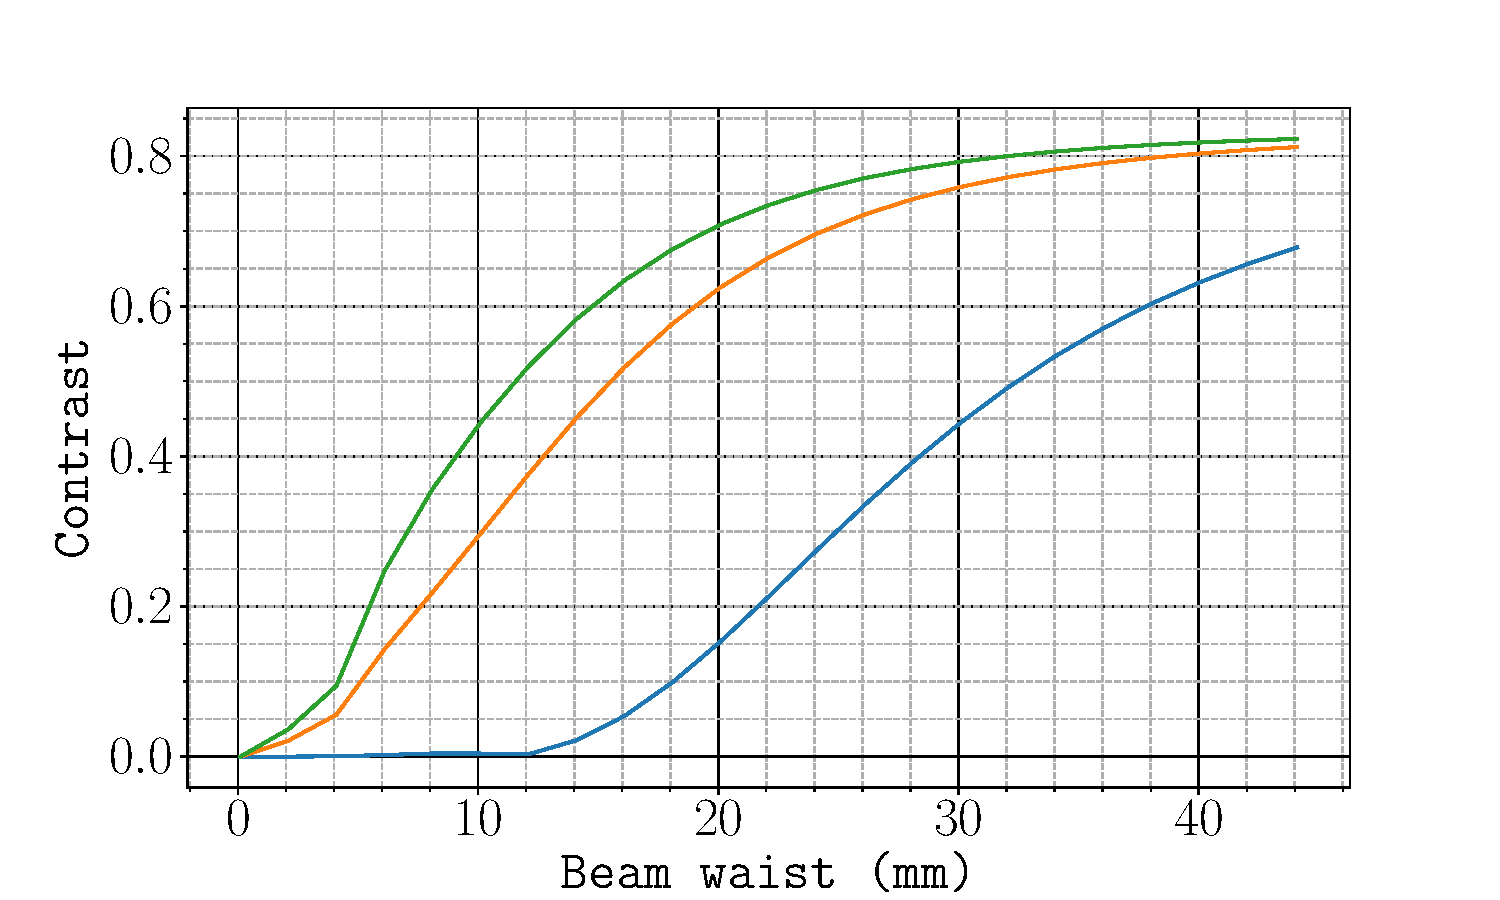
\includegraphics[width=0.5\textwidth]{fringe_contrast.pdf}
	\caption[Simulated fringe contrast vs beam waist size]{Simulated fringe
		contrast as a function of waist size \(w\) for an atom cloud falling under
		gravity. This model assumes a Gaussian distributed atomic density with a
		width \(\sigma_c = \sivalue{5}{\milli\metre}\) and a time between
		interferometer pulses of \(T = \sivalue{25}{\milli\second}\). For smaller
		beam waists the subsequent interferometer pulses have a larger intensity
		gradient across the atom ensemble, which increases the dephasing of the two
		states and reduces the interferometer fringe contrast.}
	\label{fig:raman_fringecontrast}
\end{figure}

So far, it has been shown that a large beam waist is necessary to achieve a high
fringe contrast when allowing for transverse motion of the atoms across the
laser wavefront. Otherwise, if the fringe contrast was poor, this would limit
the sensitivity of the interferometer to accelerations rather than other effects
which are less rectifiable. Another optical effect which influences the
sensitivity is distortions of the laser wavefront. In an ideal case, the
superposition of the spherical wavefronts of the two lasers results in a planar
wavefront for the effective field which drives the Raman transition. However,
propagation through rough optical elements distort these wavefronts and
introduce a spatially varying component of the Raman phase that is independent
of acceleration. If the atom cloud's trajectory is parallel with the Raman axis,
then this additional phase is the same at each laser pulse and is therefore
cancelled out. Of course, this does not occur when the cloud moves transverse to
the Raman axis where this random phase has the effect of reducing the fringe
contrast. Starting with the assumption that this phase is Gaussian distributed
around 0, with a standard deviation of \(\sigma_\phi\), if this is uncorrelated
at each interferometer pulse, then the interferometer phase \(\Delta \Phi\) will
be distributed with a standard deviation of \(\sigma_\Phi = \sqrt{6}
\sigma_\phi\). Denoting this random phase as \(\delta\phi\), the fringe contrast
is then given by
\begin{equation}
	\mathcal{C}(\delta \phi) = \cos\left(2 \delta\phi\right)
\end{equation}
Following from this, if \( \delta \phi\) is uncorrelated between each atom, the
expected value of the contrast over the ensemble is given by
\begin{align}
	\langle \mathcal{C} \rangle & = \frac{1}{\sqrt{2\pi}\sigma_\Phi}\int \mathcal{C}(\delta \phi) \; e^{-\delta\phi^2/2\sigma_\Phi^2} \; \mathrm{d}\delta\phi \\
	                            & = e^{-2 \sigma_\Phi^2}
\end{align}
The value of this expected contrast is plotted in
\FigureRef{fig:raman_phasenoise} and shows a strong dependence on
\(\sigma_\phi\). {\huge Add more justification here. Cite Achim Peter's paper}
\begin{figure}[!htbp]
	\centering
	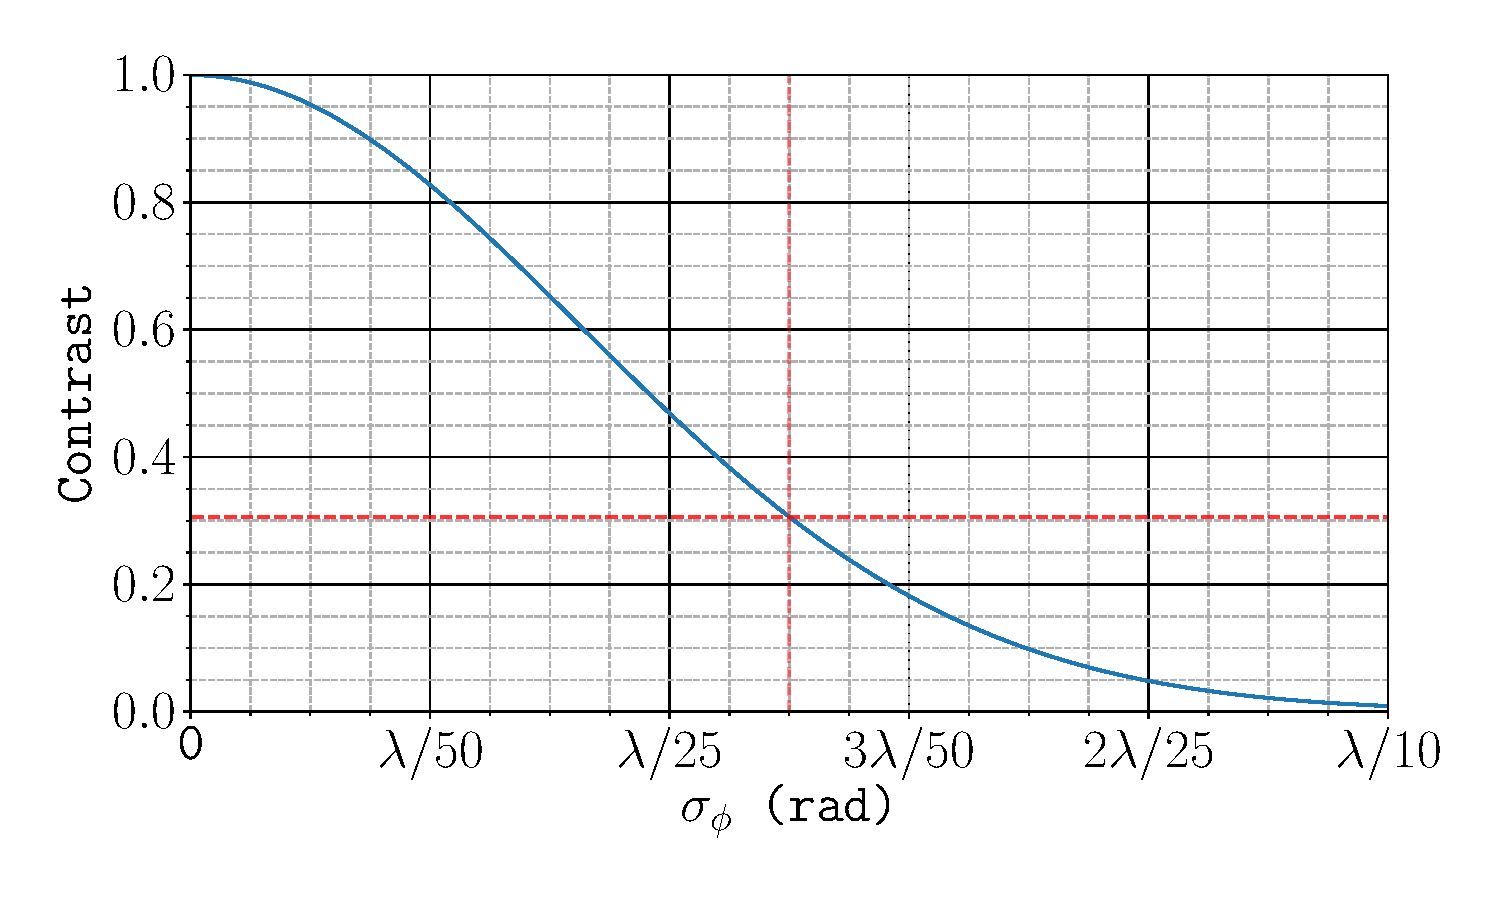
\includegraphics[width=0.5\textwidth]{phase_noise_contrast.pdf}
	\caption{Expected contrast as a function of random phase contributions. This
		assumes that the phase imprinted on an atom during each interferometer pulse
		has an additional random component that is Gaussian distributed around 0
		with a standard deviation of \(\sigma_\phi\). This random phase is also
		uncorrelated between each pulse so that the total can be obtained using
		Gaussian propagation of error. The dashed lines indicate the contrast for
		phase noise expected from conventional optics, which are usually engineered
		to a surface flatness of \(\lambda/20\).}
	\label{fig:raman_phasenoise}
\end{figure}
\subsection{Raman Beam Collimator}\label{subsec:setup_ramancollimator}
The optical system used to produce the beams for driving Raman transitions,
which will conventionally be referred to as the Raman optics, was designed to
reduce the previously mentioned effects which result in poorer interferometric
fringe visibility and sensitivity to accelerations. Principally, the entire
optical system was mounted inside the optical chamber so that the Raman light
does not pass through any optical viewports before interacting with the atoms.
Typically, the stress placed on the glass during the bonding process will
distort the flatness more than is acceptable for achieving a high contrast. For
example the viewports used for the \ac{mot} optics have a specified flatness of
\(\lambda/4\), so mounting the entire optical system inside the chamber was the
simplest way to avoid a large distortion. \par\noindent
\FigureRef{fig:raman_collimator} presents a diagram of the components used to
send Raman light into the chamber and produce a collimated beam in the centre of
the chamber. The light is coupled into the chamber using a UHV compatible
\ac{pm} fibre, manufactured by Diamond photonics. This is a kapton-coated PM-780
HP fibre that is bonded on one end to a DN16 flange using an epoxy resin. The
external side of this flange has an FC/APC connector for coupling light from
another fibre. Inside the chamber, the ferrule is connected to an FC/APC fibre
plate. This is clamped between a piece which bolts onto the inside of a DN63
flange and another stainless steel plate which bolts onto the rest of the optics
assembly. Fine adjustment of the position of the fibre along the optic axis is
achieved using shim plates with a thickness ranging from
200--\sivalue{300}{\micro\metre}. The fibre plate is free to rotate so that the
orientation of the fibre with respect to a \ac{qwp} at the output of the
collimator. This \ac{qwp} is manufactured by Light Machinery, and is described
further is \SectionRef{subsec:setup_ramanmirror}. When the fibre is correctly
orientated (e.g. when the slow axis of the fibre is at 45\(\deg\) to the slow
axis of the waveplate), the two Raman light fields are orthogonally circularly
polarised. \par\noindent The original design for the optical system consisted of
a triplet lens, as a system of three lenses is capable of correcting for the
five types of Seidel aberrations that distort rays of monochromatic light. This
was designed and manufactured by IC Optical Systems. Another specification for
this lens system was that it had to produce a collimated beam with a waist size
of around \sivalue{35}{\milli\metre} so that the sensitivity of the
interferometer was not limited by the effects of intensity gradients across the
atoms. Unfortunately, the triplet was designed with an incorrect \ac{na}. With a
focal length of \sivalue{123.4}{\milli\metre} and a diameter of
\sivalue{50}{\milli\metre}, the triplet lens has a \ac{na} of 0.194. However,
the nominal \ac{na} for PM780-HP fibre used in the UHV compatible \ac{pm} fibre
is 0.12. Consequently, the light from this fibre did not fill the \ac{na} of the
triplet lens and produced a beam with a waist of 13mm. {\huge Plot to illustrate
this}. To address this issue, a pair of aspheric lenses was included to increase
the divergence angle of light from the fibre. These are manufactured by Thorlabs
and have a focal length of \sivalue{4.51}{\milli\metre} (352230-B) and
\(\sivalue{15.29}{\milli\metre}\) (352260-B), respectively, to give a
magnification of 3.39.
\begin{figure}[!htbp]
	\centering
	\def\svgwidth{\columnwidth}
	\subfloat[][]{\scalebox{0.4}{\input{Figures/Chapter6/raman_optics.pdf_tex}\label{fig:raman_collimator}}}
	\subfloat[][]{\scalebox{0.4}{\input{Figures/Chapter6/mirror_mount.pdf_tex}\label{fig:mirror_mount}}}
	\caption[Drawings of the compenets used in the Raman optics
		assemblies]{Diagrams of the components used in the Raman optical assemblies.
		(a) shows the collimator setup. Light is coupled into the chamber using a
		UHV fibre feedthrough. A pair of aspheric lenses is used to increase the
		divergence angle of the fibre output, before the light is collimated by a
		triplet lens. Finally, a quarter-wave plate is aligned so that it circularly
		polarises the collimated light fields. (b) illustrates the other half of the
		setup, which is used to retro-reflect the light. A second quarter-wave plate
		is used so that the reflected beams have the same handedness to their
		respected incoming ones. A MEMS accelerometer is mounted on the back of the
		mirror to measure vibrations. These components are all mounted on a
		piezo-controlled mirror mount whose tilt can be controlled from outside the
		vacuum chamber.}
	\label{fig:raman_optics}
\end{figure}
\subsubsection{Alignment and Collimation}
As one of the main motivations for mounting the Raman optics inside the vacuum
chamber was to reduce the effects of wavefront distortions, it is worth
highlighting how inaccurate alignment of the optics can lead to aberrations. As
discussed before (see \SectionRef{subsec:fringe_contrast}), distortions of the
wavefront leads to a dephasing and loss of interferometer fringe visibility.
Here, the same figures of merit as before are used to consider what misalignment
is acceptable to ensure that the phase of the Raman wavefront deviates by less
than \(\lambda/100\) after a transverse distance of
\sivalue{12.5}{\milli\metre}. \par\noindent Taking the fibre as a point source,
misalignment can occur if it is displaced from the front focal point of the
optical system longitudinally along or transversely to the optic axis. If it is
transversely displaced, this manifests as an angular displacement of the
collimated light after the triplet lens. A large angular displacement is
undesirable due to the fact that since one of the Raman light fields propagates
further, the two wavefronts that drive acceleration-sensitive Raman transitions
are not parallel. \FigureRef{fig:raman_wave_transverse} shows a simulation of
the wavefront distortion as a result of this transverse misalignment. This is
obtained by simulating the propagation of rays corresponding to each Raman light
field through the optical system. The wavefront is estimated using the slope of
each ray at a distance of \sivalue{43}{\milli\metre} from the output of the
triplet lens, which corresponds to the position of the centre of the vacuum
chamber. The mirror is mounted at the same distance from the centre, so the
second beam propagates \sivalue{129}{\milli\metre}. Close to the optic axis,
this distortion is approximately linear (i.e. a tilt) and it can be seen that a
displacement of the fibre from the optic axis of <\sivalue{1}{\milli\metre} is
sufficient to achieve the desired wavefront flatness. \par\noindent Aside from a
transverse displacement, it is possible that the fibre could be misaligned along
the optic axis. In which case, the output beam will not be collimated.
Consequently, the counter-propagating reflected rays will not be antiparallel to
incoming ones. The effect of this longitudinal displacement on the Raman
wavefront is shown in~\FigureRef{fig:raman_wave_longitudinal}. Further from the
optic axis the deviation in the phase of the light is greater, giving a
quadratic distortion which is characteristic of a defocus. Comparing the
wavefront distortion in this case, a requirement on the longitudinal
misalignment of \(< \sivalue{0.6}{\milli\metre}\) is needed for the previously
specified flatness.

\begin{figure}[!htbp]
	\centering
	\def\svgwidth{\columnwidth}
	\subfloat[][]{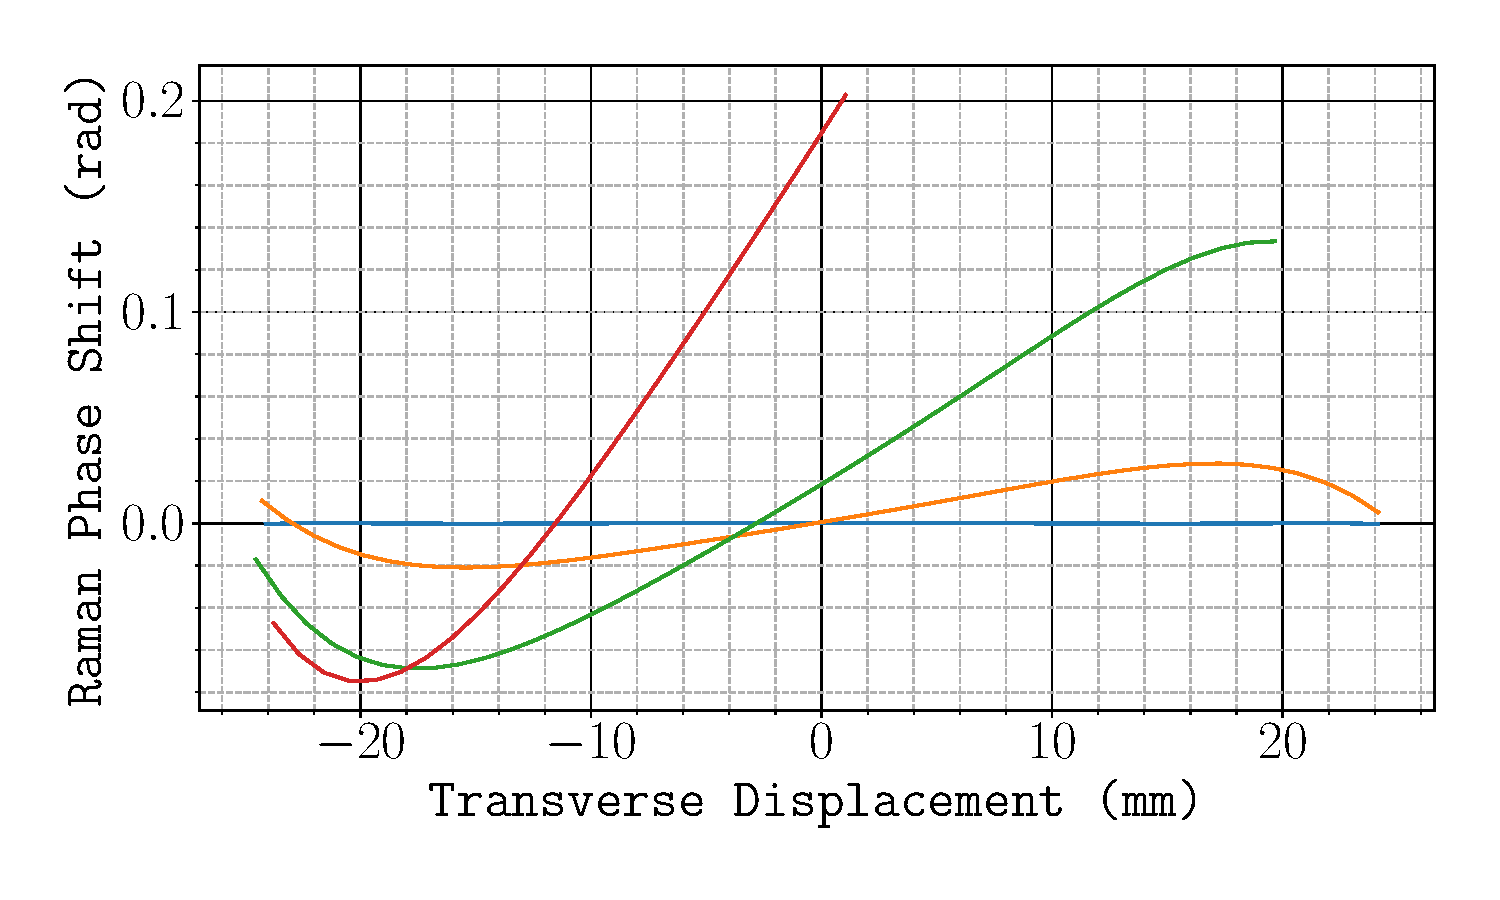
\includegraphics[width=0.4\textwidth]{wavefront_transverse.pdf}\label{fig:raman_wave_transverse}}
	\subfloat[][]{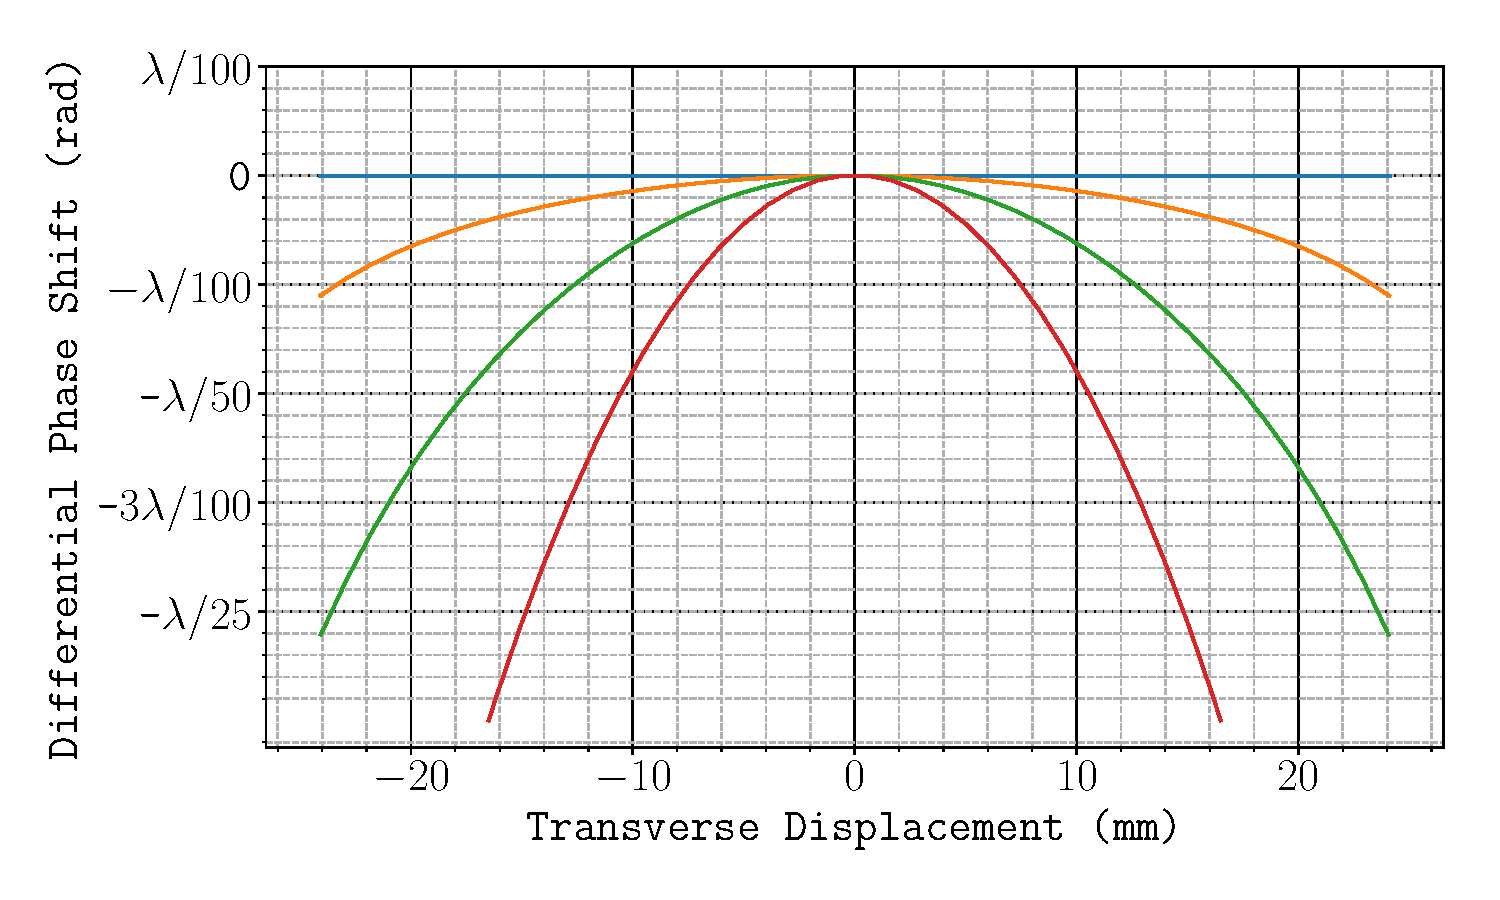
\includegraphics[width=0.4\textwidth]{wavefront_longitudinal.pdf}\label{fig:raman_wave_longitudinal}}
	\caption[Simulated wavefront distortion for longitudinal and transverse fibre
		misalignment]{Simulated wavefront distortion for longitudinal and transverse
		fibre misalignment. Rays from a point source with a divergence angle
		corresponding to a \ac{na} of 0.12 are propagated through the Raman optical
		system. Rays corresponding to the reflected beam are propagated further with
		the assumption that the mirror is perpendicular to the optic axis. The first
		set of rays propagates \sivalue{43}{\milli\metre} and the second propagates
		\sivalue{129}{\milli\metre}. The wavefront for each beam is calculated by
		taking the slope of each ray and subtracting from the slope of the central
		ray. The wavefront of the effective field that drives the Raman transition
		is the difference of these two wavefronts. (a) shows the distortion of the
		wavefront for a transverse misalignment of the fibre for a displacement of
		\sivalue{0}{\milli\metre} (blue), \sivalue{0.5}{\milli\metre} (orange)
		\sivalue{1}{\milli\metre} (green) and \sivalue{1.5}{\milli\metre} (red) from
		the front focal point. (b) shows the wavefront for longitudinal
		displacements of \sivalue{0}{\milli\metre} (blue),
		\sivalue{0.3}{\milli\metre} (orange)
		\sivalue{0.6}{\milli\metre} (green) and \sivalue{1}{\milli\metre}
		(red).}\label{fig:fig_label}
\end{figure}
\subsubsection{Measuring the Beam Width}
To measure the waist of the beam, its reflection from a flat surface was imaged
using a CCD camera. The radius of the triplet lens is smaller than the beam
waist, so the beam is apertured by this lens. To take account of this aperture,
the beam waist was estimated using a Taylor expansion of a Gaussian to second
order:
\begin{align}
	I(x) & = A e^{-\frac{(x-x_0)^2}{2 w^2}} \nonumber                                                                              \\
	     & \approx A-\frac{2 A x_0^2}{w^2}+\frac{4 A x x_0}{w^2}-\frac{2 A x^2}{w^2} + \mathcal{O}(x^3) \label{eq:gaussian_approx}
\end{align}
A typical intensity profile along the horizontal and vertical camera axes is
shown in~\FigureRef{fig:beam_examp}. A threshold intensity value excludes
contributions from pixels outside of the spatial extent of the beam. The waist
was estimated using a linear least-squares fit of the intensity profile to a
second-order polynomial \(c_0 + c_1 x + c_2 x^2\), where \begin{equation} w =
\left|\frac{\sqrt{c_1^2-4c_0 c_2}}{\sqrt{2}c_2} \right| \end{equation} A plot of
the estimated beam waist over a propagation distance of \sivalue{1}{\metre} is
shown in~\FigureRef{fig:beam_waist}. Inside the chamber each Raman beam
propagates \sivalue{5.25}{\centi\metre} and \sivalue{15.75}{\centi\metre}, where
the beam is well collimated. Along the vertical axis, the beam has a waist of
around \sivalue{36.9}{\milli\metre}. The horizontal waist is smaller because the
camera was horizontally tilted from the beam's optic axis. The projection of the
beam onto this axis is consistent with a horizontal tilt of
\sivalue{16}{\degree}.  \begin{figure} \centering
	\def\svgwidth{\columnwidth}
	\subfloat[][]{\scalebox{0.3}{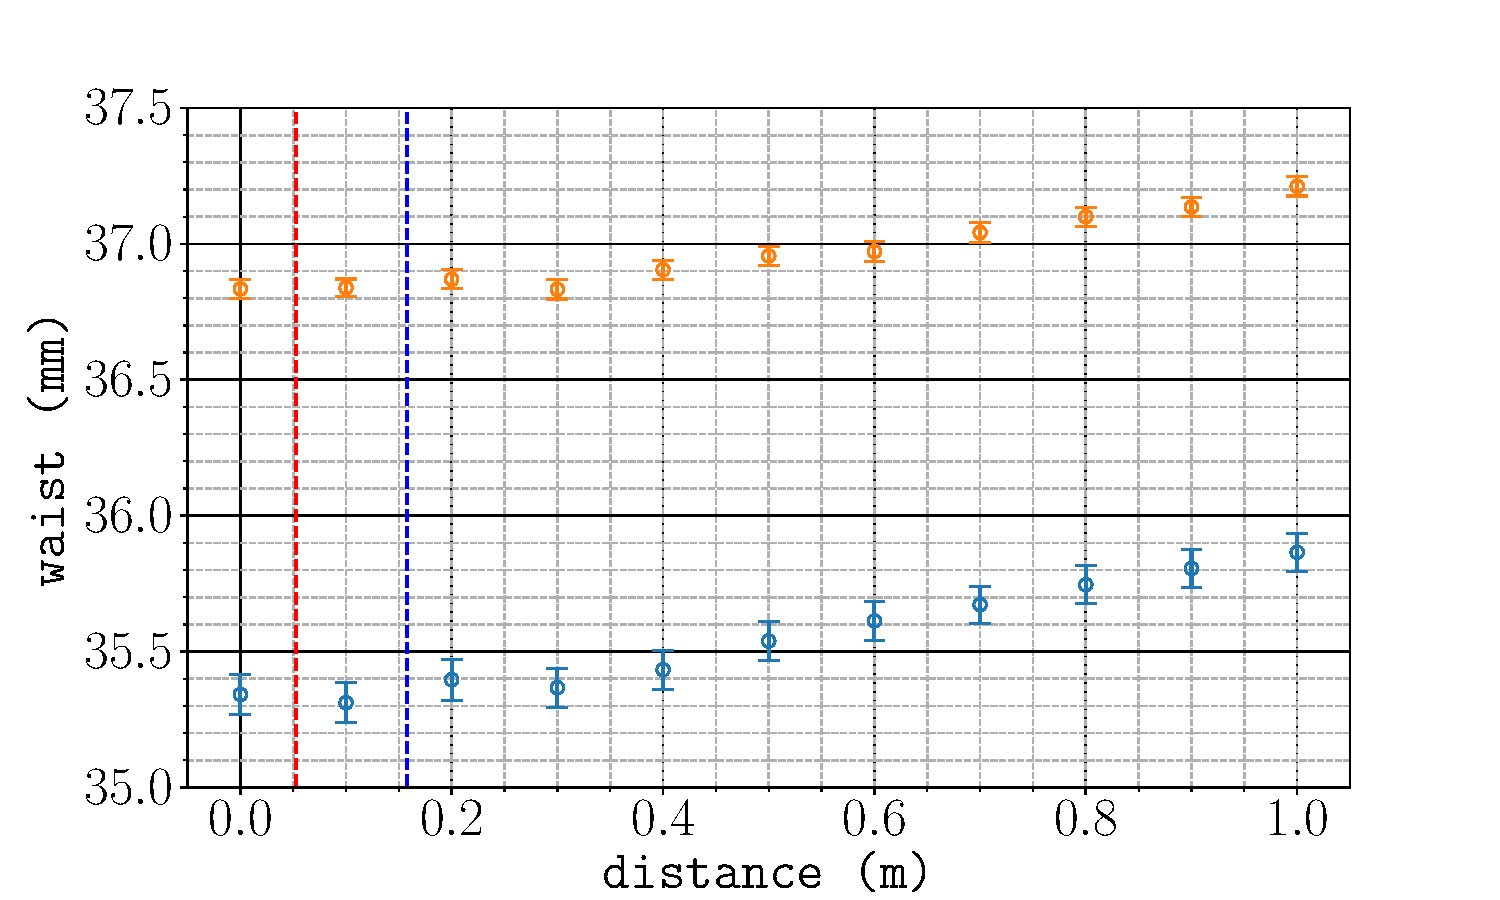
\includegraphics{beam_waist}}\label{fig:beam_waist}}
	\subfloat[][]{\scalebox{0.3}{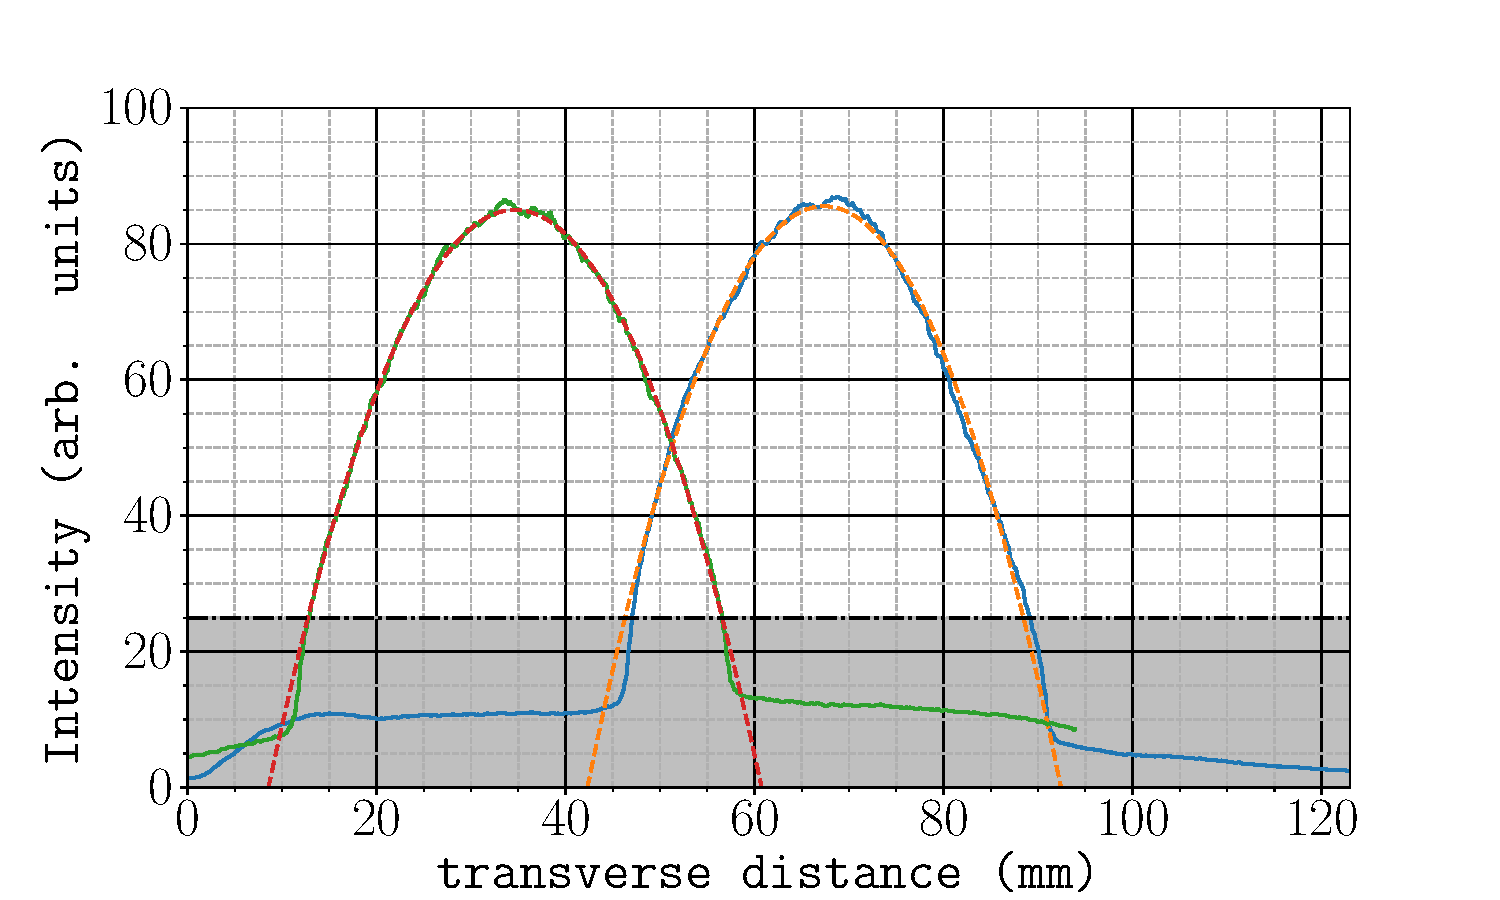
\includegraphics{beam_examp}}\label{fig:beam_examp}}
	\caption[Measured Raman beam waist]{Raman beam waist measured over a distance
		of \sivalue{1}{\metre}, shown in \textbf{(a)}. The waist along the
		horizontal and vertical axes are indicated in blue and orange respectively.
		The dashed lines indicate the approximate propagation distance of each beam
		at the position of the atoms. \textbf{(b)} shows the intensity profile along
		each axis, with the fitted parabola. The dot-dashed line is a threshold
		intensity value, which excludes pixels from outside the spatial extent of
		the beam.} \label{fig:beam_waist_plots} \end{figure}
		\subsection{Retro-reflection Assembly}\label{subsec:setup_ramanmirror} The
		Raman transitions used in the interferometer are driven by
		counter-propagating light fields to give a large momentum transfer of \(2
		\hbar k\) to the atoms. The two beams enter from the same fibre input, so a
		mirror is used to retro-reflect them. The retro-reflection assembly includes
		a \ac{qwp} to ensure that the reflected beams have the same polarisation
		handedness as their circularly polarised incoming counterpart. \par\noindent
		The mirror is also manufactured by Light Machinery, and the \ac{qwp} is made
		to the same specifications as the one that circularly polarises the incoming
		beams.  During the manufacturing process, the waveplates and mirror were
		polished to reduce irregularities in the thickness of each \ac{qwp} and the
		surface of the mirror. \FigureRef{fig:waveplate_map} shows the variation in
		the thickness of the waveplate in front of the triplet lens, measured by
		Light Machinery using a white light interferometer. This has a standard
		deviation of \sivalue{4.62}{\nano\metre} and corresponds a standard
		deviation of the optical path length of \pow{8.6}{-3}\(\lambda\).
		\begin{figure}[!htbp] \centering
	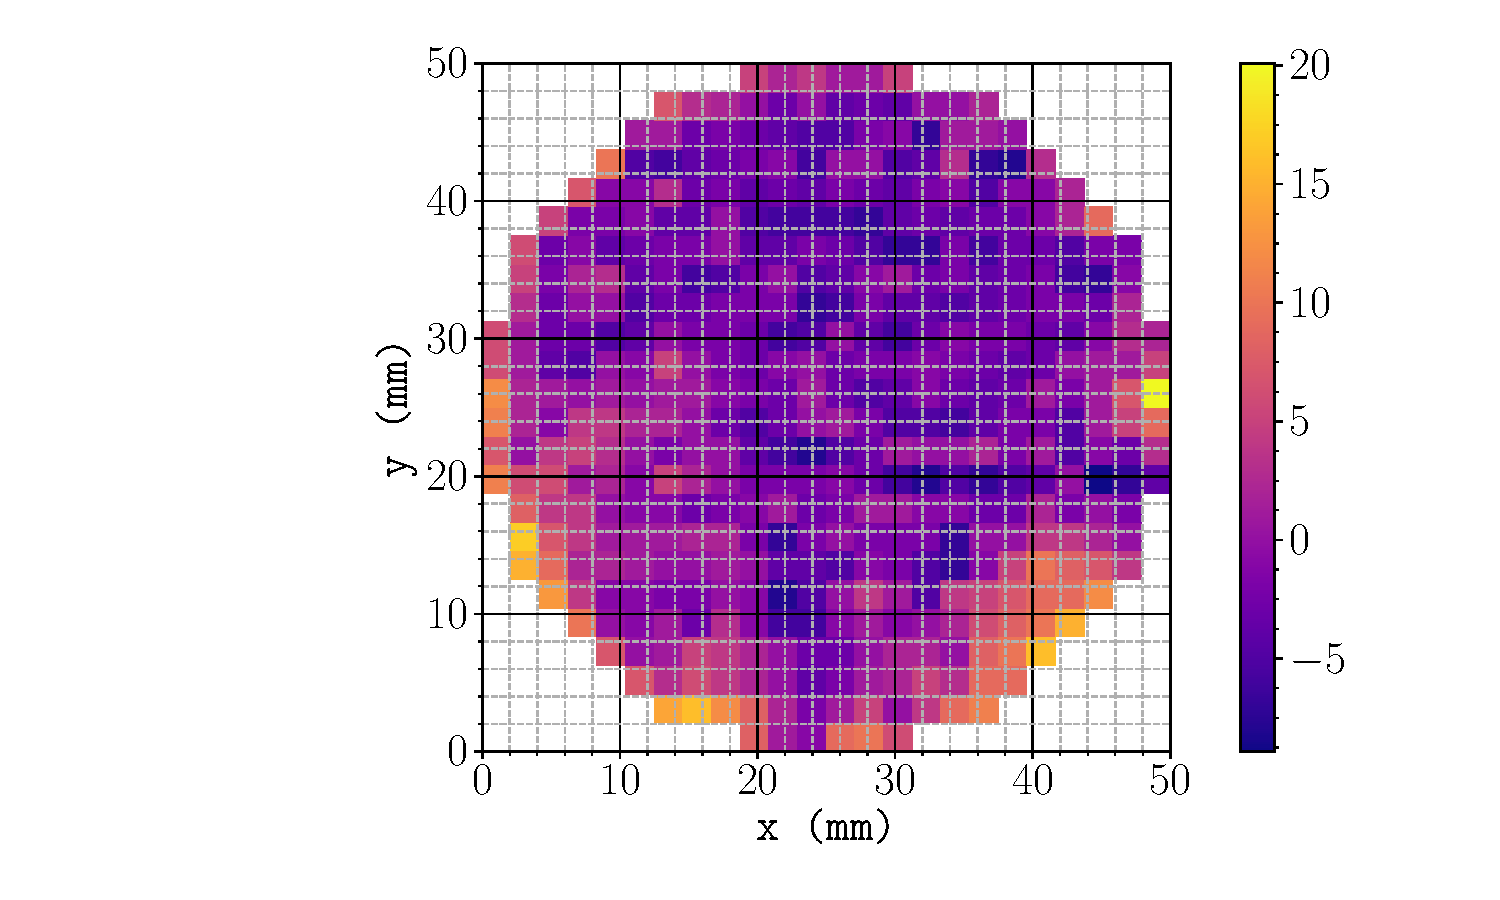
\includegraphics[width=0.5\textwidth]{waveplate.pdf}
	\caption{Thickness of the first \ac{qwp}, measured by a white light
		interferometer. The value is given in \sivalue{}{\nano\metre} as a
		difference from the mean thickness. The standard deviation of this thickness
		is \sivalue{4.62}{\nano\metre} and a peak-to-valley (PV) of {\textbf need
		number here}. Equivalent surface data for the other \ac{qwp} and mirror were
		not provided by Light Machinery, but had a PV thickness variation of
		\sivalue{19}{\nano\metre} and
		\sivalue{9}{\nano\metre} respectively.} \label{fig:waveplate_map}
\end{figure} \par\noindent The \ac{qwp} and mirror are fixed onto the front
plate of a UHV compatible MDI-HS mirror mount, manufactured by Radiant dye. The
horizontal and vertical tilt of the mirror can be adjusted using two thumbscrew
actuators which cause the front plate to pivot around a ball bearing. This mount
is designed for high stability, but of course the alignment will still drift
over time. To avoid the need to periodically open the chamber to realign the
mirror, a piezo-electric stack is placed between each actuator and the front
plate so that the tilt of the mirror can be adjusted externally. Each
piezo-stack is connected to a high-voltage feedthrough, so that their length
(and hence mirror tilt) can be finely adjusted by controlling the voltage
applied across them. A control voltage ranging between 0--\sivalue{10}{\volt} is
amplified by a controller to give an applied voltage across the piezo stack
between -10--\sivalue{150}{\volt}. This corresponds to a travel range of
\sivalue{23}{\micro\metre}. \par\noindent To understand the effect of
misalignment, it is instructive to consider its effect on the effective
wavevector \(\keff\). As illustrated in \FigureRef{fig:retro_misalign}, if the
mirror is misaligned from the incoming beam's wavevector by an angle \(theta\),
the two counter-propagating fields that drive Raman transitions have wavevectors
\(k_1 \left(1,0\right)\) and \(k_2 \left(\cos(\theta),\sin(\theta)\right)\).
\(\keff = {\textbf k_1} - {\textbf k_2} \cos (2\theta_i)\). Fortunately, for
small angular displacements, i.e. \(< \sivalue{1}{\milli\radian}\), this does
not greatly reduce the sensitivity to accelerations. In short, this means that
\(\keff\) will have a spatially varying direction. Since an atom interacting via
a Raman transition picks up a phase \(\phi = \keff . {\textbf x}\), atoms
travelling along different trajectories will accumulate different phases due to
the spatial variation of \(\keff{}\). Across the atom ensemble, this leads to a
dephasing and consequently, a loss of interferometer fringe
visibility~\cite{Tackmann2012} \subsubsection{In-Situ Alignment and
Optimisation} After mounting the Raman optical system inside the chamber, the
mirror had to be aligned to retro-reflect the light. When the mirror is close to
perpendicular to the light's wavevector, some of the power in the reflected beam
couples back into the fibre. In principle, this power is maximised when the
mirror is exactly perpendicular so maximising this power is a useful technique
to align the mirror. A 99:1 fibre splitter was used to couple light into the
chamber, which provided a means to measure the back-reflected power without
needing any free-space optics. This was set up so that 99\% of the incoming
light entered the chamber, with the other 1\% coupled into the corresponding
output port. Due to the fact that a beam-splitter acts reversibly, 1\% of the
back-reflected light which couples into vacuum fibre exits the fibre-splitter on
the other input port. Therefore, the power at this output was used to indirectly
measure the alignment of the mirror.  \par\noindent Since the travel range of
the piezo stacks does not cover the full motional range of the mirror mount, the
mirror initially had to be manually aligned using the thumbscrew actuators. Once
installed, the lack of direct access to optical system meant that conventional
methods to coarsely align the mirror, such as observing the location of the
reflected beam's focus, were not feasible. Rather than carry out the somewhat
tedious job of systematically adjusting each thumbscrew until the mirror was
aligned, an automatic routine was devised to do this. This was carried out using
a pair of bipolar stepper motors that each rotated a ball driver inserted into
the head of each thumbscrew. The revolution of these motors was controlled using
an Arduino microcontroller, which communicated to the computer using a serial
interface.  The motors rotated by 0.9\(\deg\)/step, which corresponds to a tilt
of the mirror by \sivalue{18.1}{\micro\radian}. This is smaller than the
\sivalue{0.67}{\milli\radian} angular displacement that the piezo stack could
provide, but the slow execution speed of the motor control meant that it was
more practical to use a combination of the motors and piezos to systematically
scan through the tilt of the mirror mount.  {\textbf {huge find out how big spot
size was }}. \par\noindent Using this method, the mirror mount was aligned so
that the maximum of the back-reflected power was reachable with the piezo
stacks. Of course, it was foreseeable that the mirror would need to be
periodically realigned, which would require another systematic iteration through
the voltages applied to each piezo stack. Given that this search was quite time
consuming, it was not a practical way to maintain alignment. To improve upon
this, an optimisation method using the Nelder-Mead simplex
algorithm~\cite{Nelder1965} was implemented. This method is suitable for
optimising multidimensional functions and has been used to demonstrate the
automatic alignment of a fibre with up to 6 degrees of freedom~\cite{Zhang2004}.
In general terms, this algorithm aims to optimise the value of an objective
function (in this instance, the optical power measured as a voltage by a
photodiode) by sampling the function at various locations. For \(n\) parameters,
a set of \(n-1\) points distributed randomly across the parameter space are
chosen as the initial simplex. These are sorted in decreasing order of the value
of the objective function and the algorithm proceeds by performing geometric
transformations on this simplex, by sequentially reflecting, expanding and
contracting this simplex. Each step starts with a reflection about the line
between the two greatest values. The coordinates of the simplex are updated if
the function has a greater value at the location given by one of these
transformations, until the algorithm converges on a maximum value. As with many
optimisation algorithms, the Nelder-Mead method has the potential to converge on
a local optimum, but this is alleviated by expanding the simplex to look for
more optimal values. The termination of the algorithm was decided by using the
standard deviation of the last 5 values. Empirically, it was found that
terminating when the standard deviation was less than \sivalue{10}{\micro\volt}
resulted in stable performance of the algorithm, even when the signal-to-noise
ratio of the measured voltage was poor. An example of this algorithm aligning
the mirror mount is presented in \FigureRef{fig:simplex_optimisation}. To verify
that the converged value was optimal, a systematic scan of the piezo stack
control voltages in the region around this value was also carried out. In this
case, the algorithm converged on a local maximum, but one that greatly enhanced
the coupling efficiency of the reflected light back into the fibre. The
difference in the piezo control voltages from their optimal values corresponds
to a tilt of the mirror mount along the horizontal and vertical axis of less
than \sivalue{13}{\micro\radian}.  \begin{figure}[!htbp] \centering
	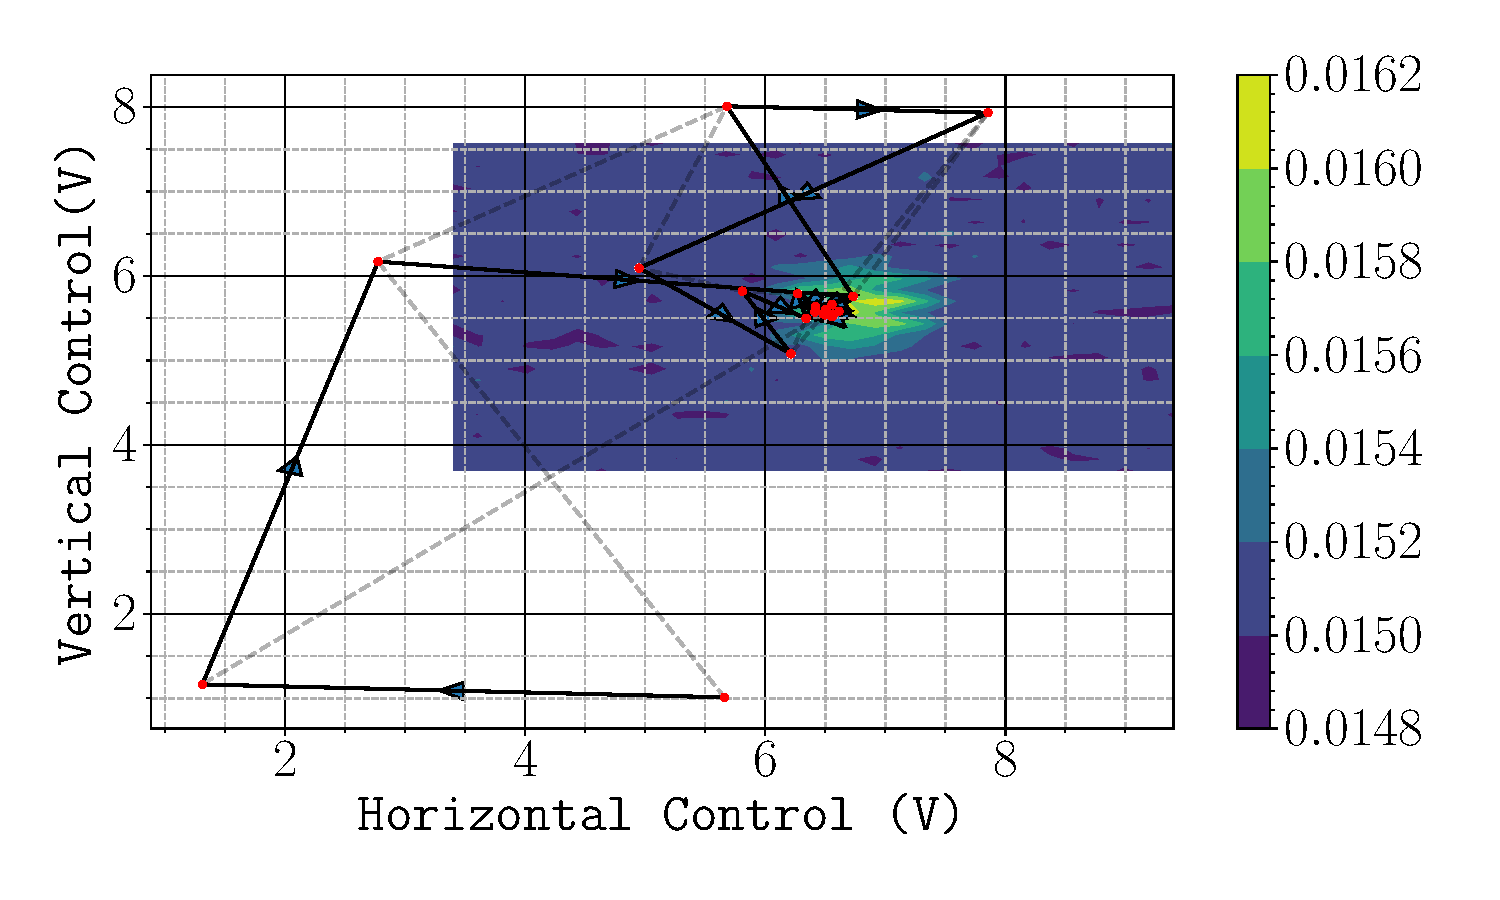
\includegraphics[width=0.5\textwidth]{simplex_alignment}
	\caption[Automatic mirror alignment using the Nelder-Mead simplex
		algorithm.]{Automatic mirror alignment using the Nelder-Mead simplex
		algorithm. This procedure starts by randomly selecting three pairs of
		control voltages for the horizontal and vertical piezo stacks. At each
		co-ordinate, the back-reflected power is measured. The algorithm proceeds by
		geometrically transforming the simplex using reflections, expansions and
		contractions, and updating the simplex using this new co-ordinate if the
		power measured is greater than the current lowest value. The algorithm uses
		the standard deviation of the last 5 values as a check for convergence. In
		this case, it terminates once the standard deviation is smaller than
		\sivalue{10}{\micro\volt}. The shaded lines indicate the simplex bounded by
		the three co-ordinates at each iteration, whose area reduces as the
		algorithm converges on the optimum value. A scan of the piezo control
		voltages close to the optimum is also plotted. The irregular shape of the
		measured power is a result of a hysteresis effect when the horizontal
		control voltage was changed from its maximum value to the minimum. Even with
		a low signal-to-noise ratio, the algorithm converged on a value close to the
		optimum. This resulted in a misalignment of less than
		\sivalue{13}{\micro\radian} along both axes.}
		\label{fig:simplex_optimisation} \end{figure}
\subsection{The Mechanical Accelerometer}\label{subsec:raman_mems}
The periodic interferometer signal means that the interferometer phase is only
proportional to acceleration over one fringe spacing \(\Delta a =
\frac{\pi}{\keff T^2}\). Furthermore, the fringe spacing is inversely
proportional to \(T^2\) so there is a trade-off between dynamic range and
sensitivity. These problems can be addressed by making use of a mechanical
accelerometer mounted onto the back of the retro-reflecting mirror to form a
hybrid system~\cite{Lautier2014}. The accelerometer determines the acceleration
up to the fringe spacing  and the interferometer measures the acceleration more
precisely. The accelerometer also measures the vibrations of the
retro-reflecting mirror, so it can be used to filter the effects of vibration
noise on the interferometer signal. This is discussed in more detail
in~\SectionRef{sec:vibration_sensitivity}. This hybridisation scheme has been
used in measurements of gravity in high noise environments such as the centre of
Paris~\cite{Merlet2009} and in parabolic aircraft
flights~\cite{Geiger2011a,Barrett2016a}. \par\noindent The accelerometer is a
navigation-grade AI-Q-2010 manufactured by \textit{Innalabs}. This particular
device was chosen because its specified intrinsic noise was
<\sivalue{7}{\micro\g} in the 0-100\ac{Hz} bandwidth. For a pulse separation \(T
= \sivalue{25}{\milli\second}\), the fringe spacing is
\(\sivalue{31.2}{\micro\g}\) so it is sensitive enough to measure the
acceleration to within one fringe. A schematic of this device is shown
in~\FigureRef{fig:innalabs}. It operates using a quartz pendulum which is is
free to move about one axis~\cite{Foote1992}. Under an acceleration, the
deflection of the pendulum is capacitively detected. A servo loop circuit drives
a current through the coils to restore the position of the pendulum. This
current is directly proportional to the acceleration of the pendulum. This model
has a nominal scale factor of \sivalue{1.235976}{\milli\ampere\per\g}. The
acceleration is measured using a load resistance of \sivalue{6}{\kilo\ohm} to
give an output voltage of \sivalue{7.56}{\volt\per\g}.
\begin{figure}[!htbp] \centering
	\resizebox{0.5\textwidth}{!}{\input{innalabs.pdf_tex}}
	\caption[Innalabs accelerometer cross-section]{Cross-section of the Innalabs
		AI-Q-2010 accelerometer.} \label{fig:innalabs}
\end{figure}
\section{The M-Squared Laser System}\label{sec:msquared_laser} 
  This section describes the laser system manufactured by \textit{M-Squared
  Lasers}, which is used to drive Raman transitions. An overview of the laser
  system can be found in~\SectionRef{subsec:msquared_overview}, which includes
  the techniques used to externally communicate with the laser's ICE-BLOC
  control modules. The control of the frequency and phase-lock is then described
  in~\SectionRef{subsec:msquared_control}. Finally, this section concludes
  in~\SectionRef{dcs_module} with a description of the module used to control
  the output of the laser in real-time.
\subsection{Laser System Overview}
\label{subsec:msquared_overview} This system contains two Solstis lasers which
generate laser light by pumping a Ti-sapphire crystal housed inside a resonator.
The output light frequency is controlled using piezo-electric stacks to adjust
the resonator length. A schematic diagram of this laser system is given
in~\FigureRef{fig:msquared_laser}. Each laser is seeded using a
\textit{Lighthouse Photonics} Sprout laser to generate light around
\sivalue{780}{\nano\metre}. The first laser acts as the master whose frequency
is fixed. The second is slaved to this using a phase-locked loop to keep their
beat frequency and relative phase constant. The two beams are mixed on a
\ac{pbs}, so that they are orthogonally polarised. Two \acp{aoms} control the
output power. A planned upgrade for this system will have multiple output ports
for the Raman light, which will require independent control. \par\noindent The
system contains 4 ICE-BLOC modules which implement various types of control. The
first two (one for each Solstis) are used to stabilise the output power of each
laser by feeding back to the corresponding Sprout laser. They are also used to
coarsely adjust the output frequency using a
\textit{HighFinesse} wavemeter. The third is used for the \ac{pll}
and feeds-back onto the slave laser to control both the frequency and phase of
the optical beat-note between the two lasers. The final ICE-BLOC, referred to
as the DCS module, is used to control the lasers in real-time during the
experiment.  \begin{figure}
	\centering \fontsize{10pt}{10pt}
	\resizebox{0.4\textwidth}{!}{\input{msquared_laser.pdf_tex}}
	\caption[M-Squared Laser System Schematic]{Schematic Diagram of the M-Squared
		laser system. Two Solstis lasers provide the two Raman frequencies, which
		are fibre coupled onto the orthogonal axes of a \ac{pm} fibre. Control of
		the power, frequency and phase as required to drive Raman transitions is
		handled by the four ICE-BLOC modules indicated in blue. Further detail of
		this control is given in the text.} \label{fig:msquared_laser}
\end{figure}

\subsubsection{External ICE-BLOC Control}
The ICE-BLOC modules are able to communicate with each other using an Ethernet
hub. Another computer connected to this network is able to control them by
accessing a web page that each module hosts. These web pages control the ICE-BLOCs
by sending structured JSON messages. This graphical interface can be bypassed by
directly communicating these messages. This is done using MOTMaster so that
various parameters, such as the frequency and phase of the Raman beat-note, can
be automatically varied between each experiment cycle. \subsection{Frequency and
Phase Control}\label{subsec:msquared_control}

\subsubsection{Master Lock}
The frequency of the master laser is stabilised using saturated absorption
spectroscopy in a rubidium vapour cell. Part of the beam is picked off and
modulated by an \ac{eom}. The positive frequency sideband is used to lock the
master laser to the 2,3 crossover feature. In effect, this means that the
modulation frequency of the \ac{eom} sets the one-photon detuning of the Raman
transition. The modulation frequency is set so that the master laser frequency
is \sivalue{1.13}{\giga\hertz} below the \trans{2}{3} transition.

\subsubsection{Frequency and Phase Lock} The optical beat-note between the two
lasers is measured using a fast photodiode. The signal from this is used in a
phase-locked loop to fix the relative phase between the two lasers. A frequency
divider halves the frequency of the signal before comparing it to a \ac{vco} of
around \sivalue{3.4}{\giga\hertz}. This creates an error signal which used to
control both the frequency and phase of the beat-note by feeding back to the
slave laser Solstis. The relative phase between the two lasers is adjusted using
an analogue phase shifter and the frequency difference is controlled by tuning
the \ac{vco} frequency. \par\noindent The beat-frequency of the Raman lasers can
be chirped by triggering a ramp of the control voltage to the \ac{vco}. For
chirp rates of lower than \sivalue{24}{\mega\hertz\per\second}, the phase-lock
is able to keep the beat-note phase-coherent during the chirp.  \subsection{The
DCS Module}\label{subsec:dcs_module} The DCS module is used to control the
output of the lasers during the experiment. It uses an on-board \ac{DDS} to
synthesise the \sivalue{80}{\mega\hertz} driving frequencies for each \ac{aom}.
The majority of the control is done using an \ac{fpga} that synthesises a timed
sequence of analogue and digital voltage waveforms. An example of a sequence
created using the DCS web interface is shown in~\FigureRef{fig:dcs_module}. The
sequence is segmented into individual steps and each channel can be separately
configured, much like the MOTMaster user interface. \par\noindent This module is
used to control the amplitude, frequency and phase of each Raman pulse. The
pulse amplitude is shaped using an analogue voltage to control the power of the
RF frequency. This has been calibrated so that the pulse can be shaped to
produce a square, Gaussian or Blackman amplitude envelope. A frequency chirp is
optionally triggered by sending a digital pulse to the \ac{pll} ICE-BLOC.
\par\noindent The synthesiser can be configured to run continuously, or to wait
at a chosen timestep for an external trigger. It can also iterate through a set
number of parameters, such as timestep duration or phase shift by re-building
the sequence after each cycle.  \begin{figure}[!htbp] \centering
	\resizebox{0.5\textwidth}{!}{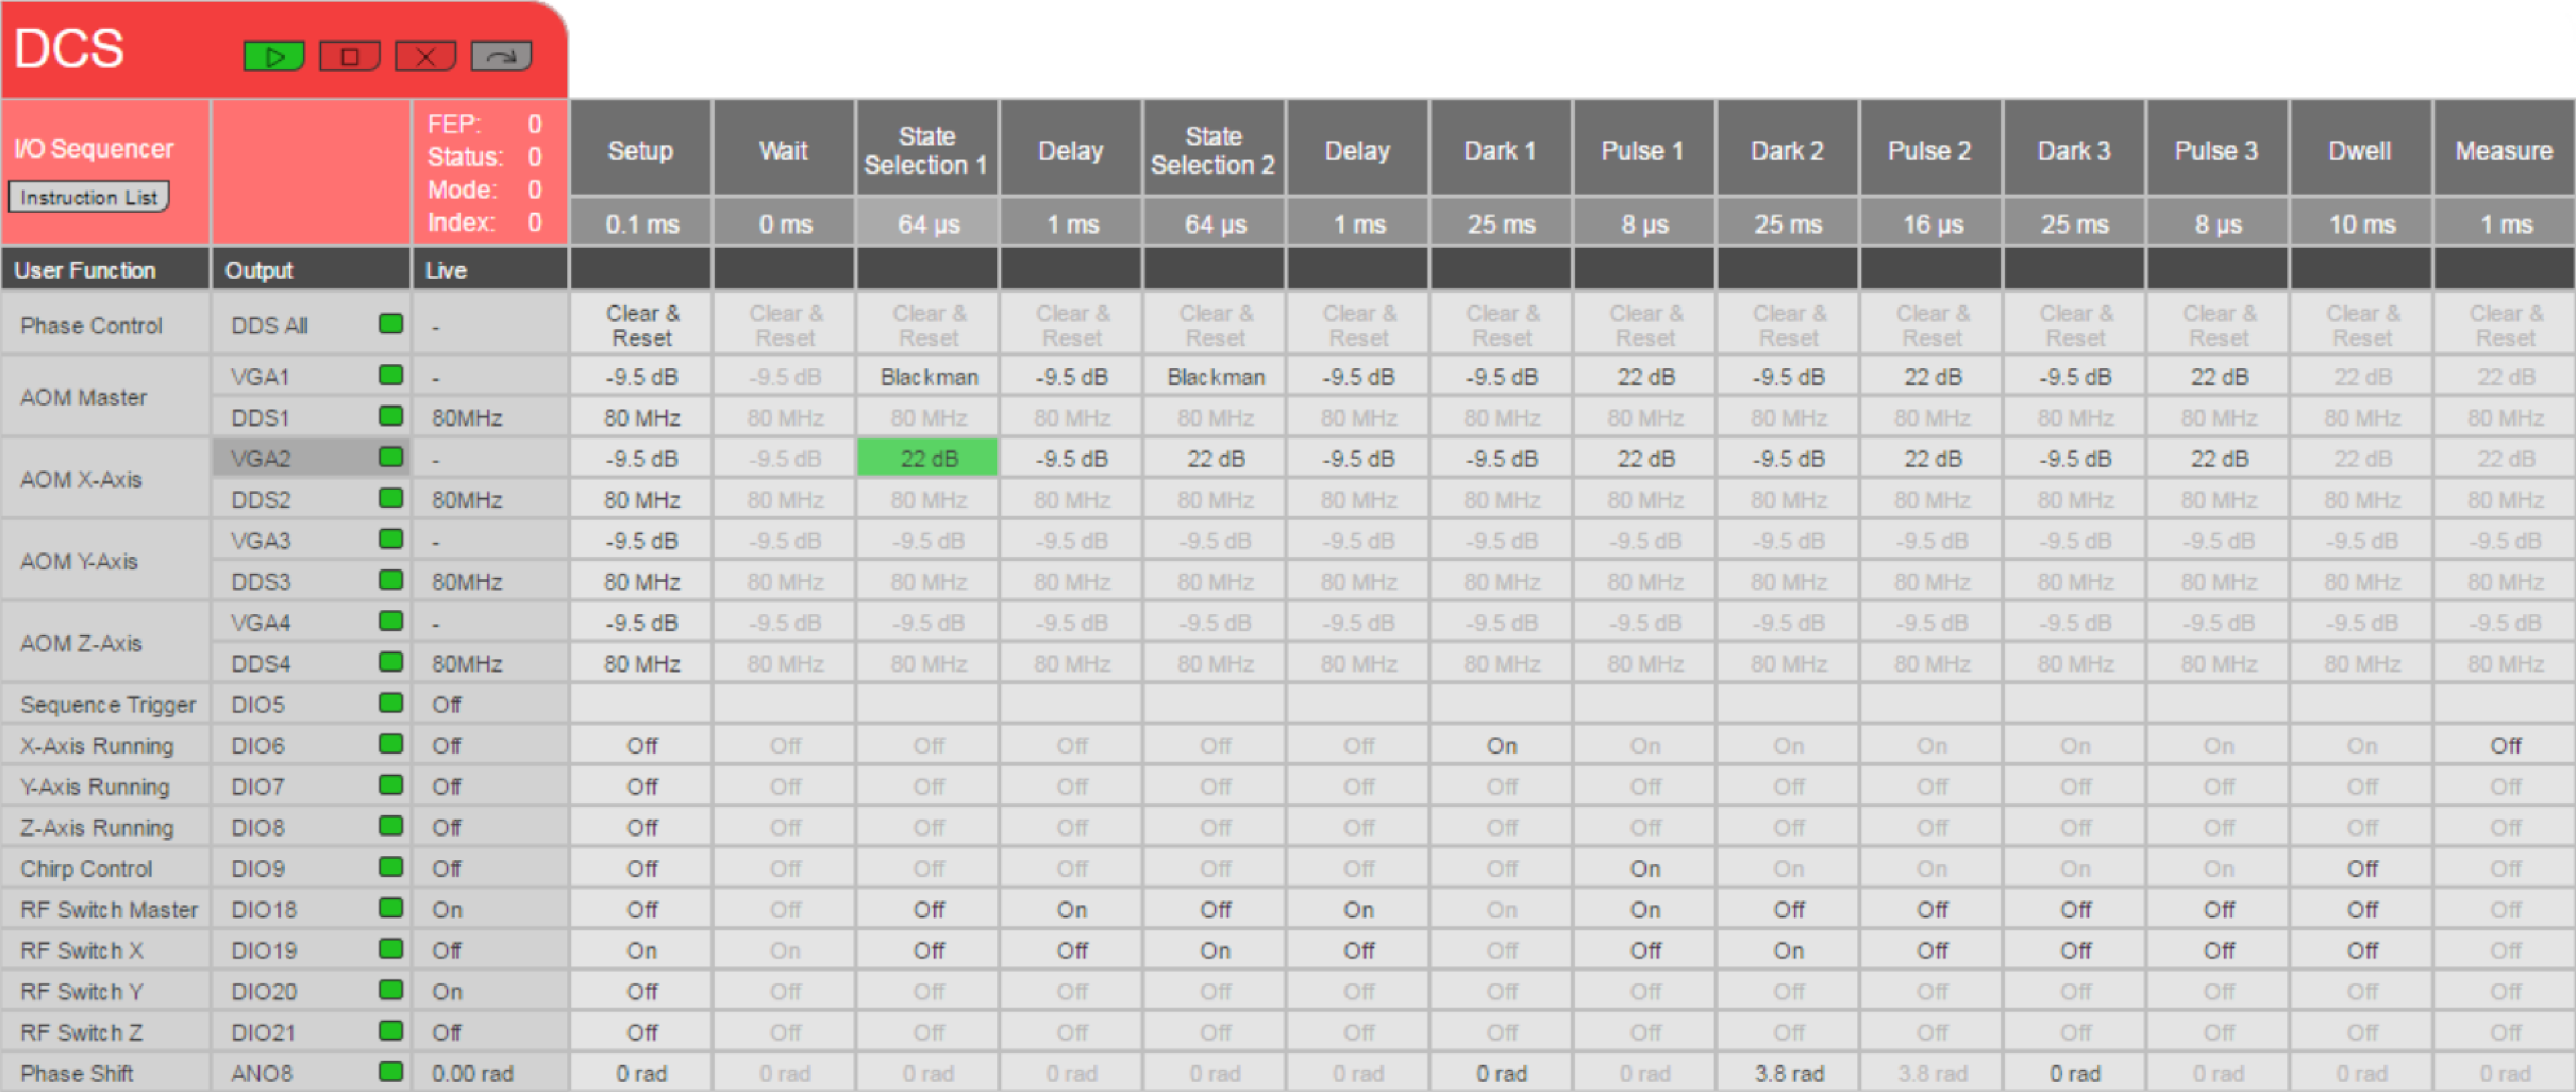
\includegraphics{dcs_module.pdf}}
	\caption[DCS Module User interface]{DCS module user interface. The sequence is
		synthesised from individual steps, The parameters of each Raman laser pulse
		can be configured independently.} \label{fig:dcs_module} \end{figure}
\section{Atom Detection}\label{sec:atom_detection} 
\begin{itemize} 
  \item Photodiode system - diagram 
  \item Detection sequence - diagram 
  \item Statistical analysis to estimate phase from measured voltages 
  \item Simulate detection curves?  
\end{itemize} 
This section describes the methods used to
measure the number of atoms in each hyperfine ground state. It begins with a
presentation the other optical components used to detect the atoms by
driving \(\sigma^+\) transitions in~\SectionRef{subsec:photodiode_setup}.
The sequence of light pulses used to measure the number of atoms is then
given in~\SectionRef{subsec:detection_sequence}. This concludes with a
discussion on converting the measured photodiode signals into atom
number and interferometer phase.
\subsection{Optical Setup}\label{subsec:optical_setup}
A precise measurement of the number of atoms requires that the atom shot noise
is the dominant source of uncertainty in the measurement. The CCD used in
previous stages of the experiment is not sensitive enough for this as there is a
significant amount of noise in reading out the charge collected at each pixel.
Instead, a more sensitive photodiode is used to detect the atoms. With a
suitably high bandwidth, the readout time is much faster than the CCD as well,
so that the atoms can be detected well before they fall out of the field of
view. \par\noindent A diagram of the setup used to detect the atoms is given
in~\FigureRef{fig:photodiode_optics}. It is a triplet system which uses an
lenses with focal lengths \sivalue{150}{\milli\metre},
\sivalue{75}{\milli\metre} and \sivalue{60}{\milli\metre} in order from the
atoms to the photodiode.  A ray-tracing simulation of the optical
system indicates spherical aberrations on the image. This is caused by
the third lens, which was added to shorten the back focal length. The
front lens has a diameter of
\sivalue{50.4}{\milli\metre}, so the solid angle subtended by the
optics is \(4\pi \times\)\num{7.056e-3}\si{\steradian}.

\subsubsection{Photodiode Calibration}
The photodiode used is a \textit{Femto LCA-S-400K-SI},
which has a trans-impedance amplifier with a bandwidth of \sivalue{400}{\kilo\hertz} and a photo-sensitive area
with a diameter of \sivalue{3}{\milli\metre}.
A calibration of the output voltage for an input collimated beam is
shown in~\FigureRef{fig:photodiode_calib}. This
gives a conversion factor of \sivalue{1.84e6}{\volt\per\watt}.
\subsection{Detection using \(\sigma^+\) transitions}\label{subsec:photodiode_setup}
The atoms are detected using resonance fluorescence from two of the
circularly polarised \ac{mot} beams. A bias field polarises the atoms along the
\(\vec{z}\) axis, so that the light drives both \(\sigma^+\) and \(\sigma^-\)
transitions. Each Zeeman state has a different scattering rate, which
must be accounted for to calculate the number of atoms. This can be
simplified by flipping the handedness of
one of the \(\vec{z}\) \ac{mot} beams using a liquid-crystal
\ac{hwp}, so that both beams drive \(\sigma^+\) transitions. Now, the
atoms are optically pumped into \(\ket{2,2}\) and cycle on the
\(\ket{2,2} \rightarrow \ket{3,3}\) transition. Only this scattering
rate is required to determine the number of atoms.
\par\noindent
\FigureRef{fig:detection_scheme} shows the setup used to invert the
polarisation of one \ac{mot} beam for detection. The liquid-crystal waveplate is an electro-optical device whose birefringence changes when an ac voltage is applied across it. The waveplate is placed at the output of the downward-propagating (\(\vec{z}_-\))
collimator. 
  \begin{figure}[!htpb]
    \centering
    %    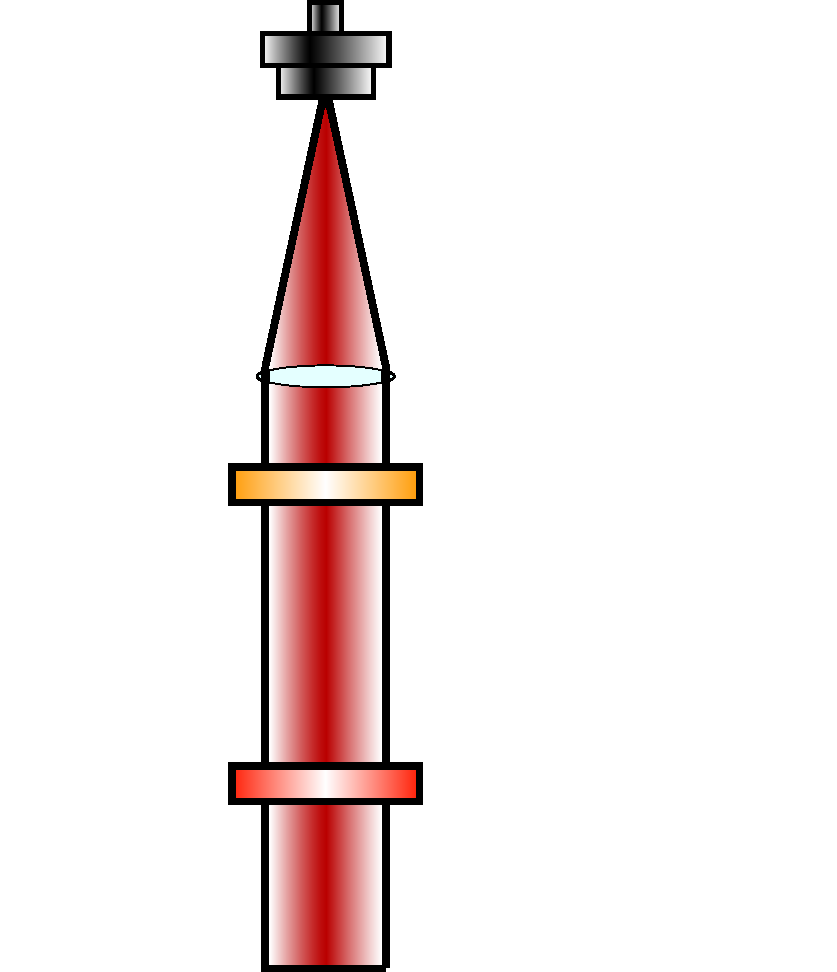
\includegraphics{detection_scheme.pdf}
    \caption{Scheme for detection by driving \(\sigma^+\) transitions. A
      liquid-crystal waveplate flips the handedness of the \(\vec{z}_-\) \ac{mot} beam. The atoms then fluoresce on the \(\ket{2,2} \rightarrow \ket{4,3}\) cycling transition}\label{fig:detection_scheme}
\end{figure}
\begin{figure}[!htbp] 
  \centering \fontsize{18pt}{18pt}
	\resizebox{0.7\textwidth}{!}{\input{photodiode_optics.pdf_tex}}
	\caption[Optical setup for Photodiode Detection]{Optical setup for photodiode
		detection. A triplet lens system focuses light from radiated from the atoms
		onto a photodiode. This is mounted using a translation stage to
  position the photodiode at the back focal point.}
  \label{fig:photodiode_optics}
\end{figure}
\subsubsection{Detection Sequence}\label{subsec:detection_sequence}
The sequence used to detect the atoms is shown
in~\FigureRef{fig:detection}. Shortly before the sequence starts, the
bias field is aligned to the \(\vec{z}\) axis and the liquid-crystal
waveplate is triggered to change the handedness of the \(\vec{z}_-\)
beam. The cooling laser frequency is set so it is detuned by
\(\delta_D =\) \sivalue{3}{\mega\hertz}
below the \trans{2}{3} transition and the repump laser is set to
resonance with the \trans{1}{2} transition. This creates an optical
molasses which avoids heating the atoms so that they remain in the
detection volume for a longer period of time. The intensity of the
light is reduced to around \(3 I_\text{sat}\). As shown below, this
intensity was empirically found to minimise the variance in output
voltage. The acquisition of the photodiode voltage is
triggered to start at the first Dwell time. The cooling light is first
switched on, so that only atoms in \(\ket{F=2}\) scatter light. After this, the repump
is switched on, so that atoms in \(\ket{F=1}\) are optically pumped
into \(\ket{F=2}\) and all the atoms scatter light. This repump light is a
sideband of the cooling laser, so the total output is increased
to ensure that the intensity of the cooling light remains constant.
Each detection step lasts \sivalue{250}{\micro\second}, but the
first \sivalue{50}{\micro\second} is discarded to allow time for the
intensity to stabilise and for optical pumping into \(\ket{F=2}\).
The atoms are then blown away by switching off one of the detection
beams before the sequence is repeated to collect a
background signal.
\begin{figure}[!htbp] 
  \centering
  \resizebox{0.7\textwidth}{!}{\input{detection.pdf_tex}} 
  \caption[State detection sequence timing]{Timing diagram for state
  detection. Atoms in \(\ket{F=2}\) are detected before the repump
light pumps those in \(\ket{F=1}\), so they are detected as well. A
background light measurement for each step is also taken.}
	\label{fig:detection} 
\end{figure}
\subsubsection{Maximum Detection Time}\label{subsubsec:intensity_dependendce}
As the atoms scatter light during detection, the cloud will be heated
and expand due to the momentum exchanged from absorption and
spontaneous emission. The atoms are only cooled along the axis of the
detection beams, so the heating rate is greatest along the other two
axes. It is necessary to ensure that the
heating rate is low enough that the atoms remain within the
detection beam for the entire detection time. A requirement on the
maximum detection time can be obtained as follows. The momentum of
an atom scattering photons follows a random walk, so the variance of
the momentum along one axis after a time \(t\) is
\(\langle\Delta p\rangle^2 = 2 D t\). The scattered photon is equally
likely to be emitted in any direction, so the diffusion coefficient is
\begin{equation}
  D = \frac{1}{3}(\hbar k)^2 R_\text{sc}
  \label{eq:diffusion_coeff}
\end{equation}
If the cloud has a
Gaussian spatial distribution with an
initial width of \(\sigma_0\), the width at a later time of
is given by
\begin{equation}
\sigma_x^2(t) = \sigma_0^2 + \frac{2 n_p v_r^2 t^2}{3} 
  \label{eq:width_scattering}
\end{equation}
where \(v_r = \frac{\hbar k}{m_\text{rb}} =
\)\sivalue{6}{\milli\metre\per\second} is the recoil velocity and \(n_p\) is the
number of photons scattered. To remain within the detection region,
the width of the cloud must be smaller than the detection beam waist
\(w\), so the detection time must satisfy
\begin{equation}
  t_D \ll \sqrt{\frac{3 \left(w^2-\sigma_0^2\right)}{2 \left(n
  v_r^2\right)}}
  \label{eq:detection_time}
\end{equation}
For a beam waist of \sivalue{7.5}{\milli\metre}, initial cloud size of
\sivalue{5}{\milli\metre} and a maximum scattering rate of
\sivalue{2e7}{\per\second} the detection time must be much less than
\sivalue{4.7}{\milli\second}. 
%\begin{equation}
%  p(x,t) = \int \frac{1}{\sqrt{2\pi} e^{-\frac{(x + \frac{p}{m}
%    t)^2}}{2 \sigma_x^2} \frac{1}{\sqrt{2\pi D t} e^{-\frac{p^2}{2 D
%      t}} \mathrm{d}t
%  \label{eq:prob_atom_diff}
%\end{equation}
\subsubsection{Optimal Intensity}
The optimal intensity was empirically found by varying the total power
in the detection beams and recording the photodiode voltage for a
fixed detection time of \sivalue{200}{\micro\second}.
\FigureRef{fig:photodiode_intensity_calib} the average voltage
measured by detecting atoms in the \(\ket{F=2}\) state as the
intensity of the light increases. The saturation parameter \(s\) is
defined using the peak intensity and by the time they are detected,
the atoms have moved from this region. A non-linear least squares fit
to the function
\begin{equation}
  v = a\frac{b s}{1 + b s + 4 \left(\delta_D/\Gamma\right)^2}
  \label{eq:voltage_fit}
\end{equation}
gives a scaling for the intensity of \(b = 0.83\). The variance in the
measured voltage (for a constant mean number of atoms) is minimised when the
intensity is around 3\(I_\text{sat}\). Above this intensity, there is
a significant depopulation into \(\ket{F=1}\) caused by off-resonant
excitations to the \(\ket{F'=2}\) state.
This is clearly evident in the voltage signal over time, which is
shown in \FigureRef{fig:detection_time} for various intensities. At an
intensity of 3\(I_\text{sat}\), around 5\% of the population is
pumped out of \(\ket{F=2}\).
\begin{figure}[htpb!]
  \centering
  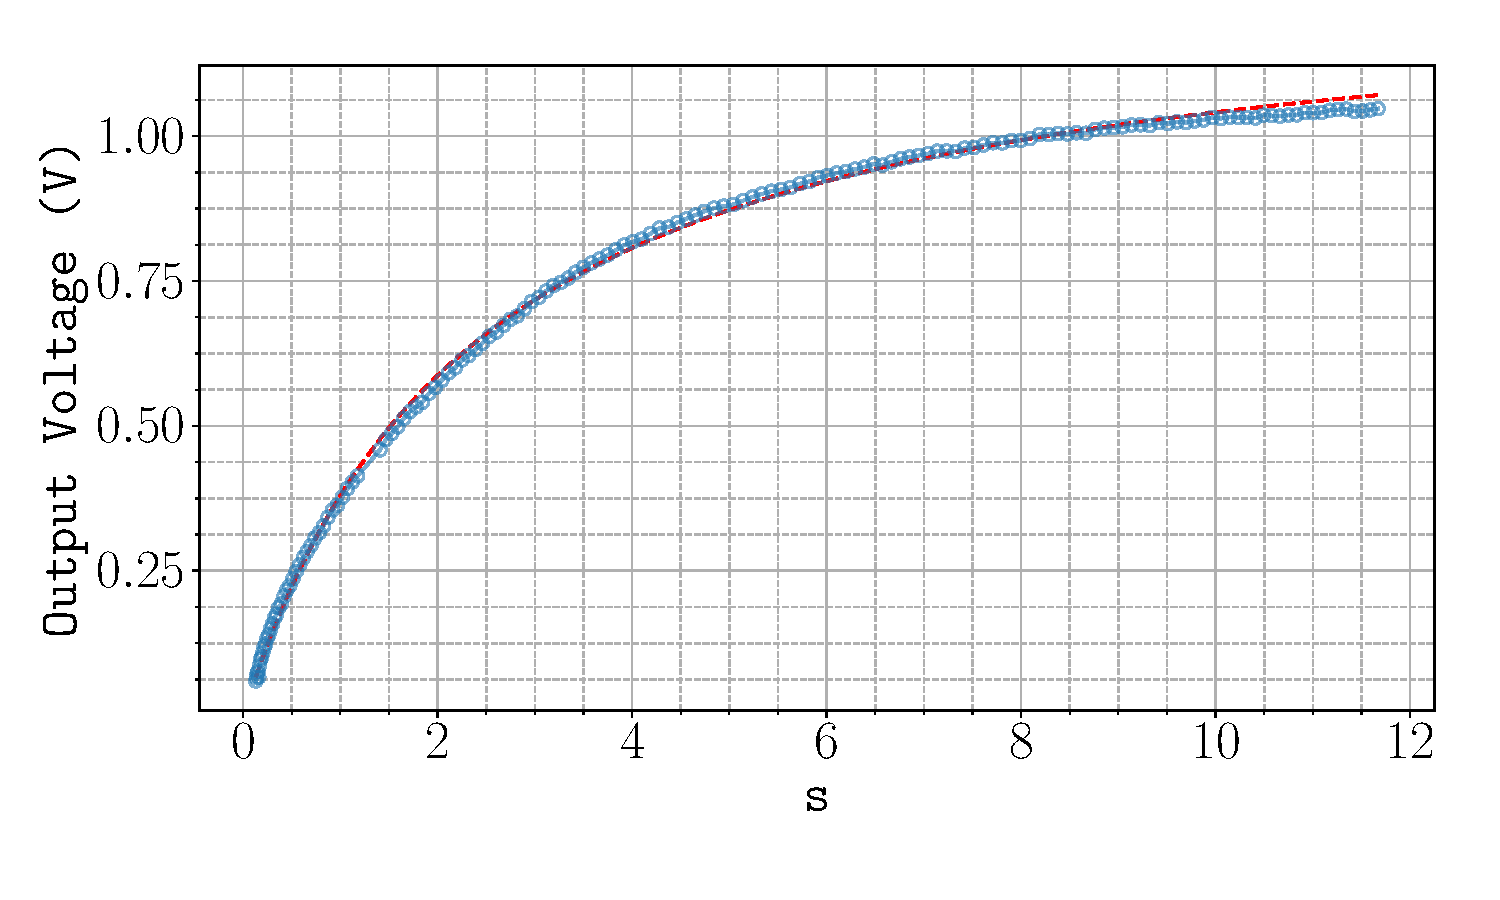
\includegraphics[width=0.7\textwidth]{photodiode_intensity}
  \caption{Photodiode output voltage for increasing detection beam
  intensity. The red dashed line indicates a fit
to~\EquationRef{eq:voltage_fit} to estimate the scaling factor for the
saturation parameter \(s\).}
  \label{fig:photodiode_intensity_calib}
\end{figure}

\begin{figure}[htpb!]
  \centering
  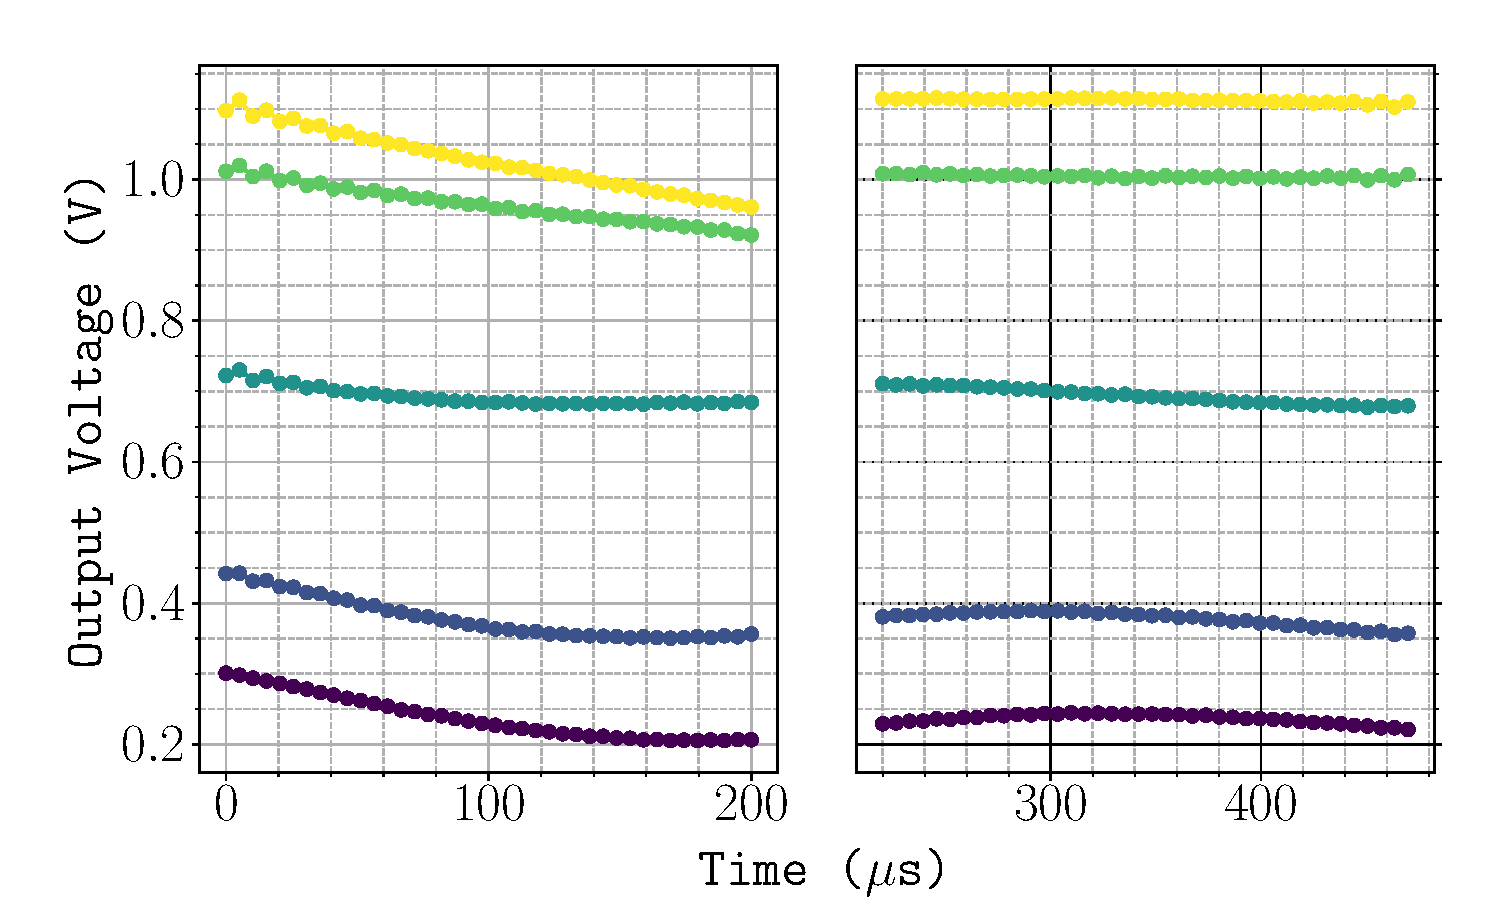
\includegraphics[width=0.7\textwidth]{photodiode_voltage_time}
    \caption{Photodiode voltage over time during detection for \(s =
    0.5, 1, 3, 7, 10\) in order from purple to yellow.}
  \label{fig:detection_time}
\end{figure}

\subsection{Measuring the Occupation Probability}\label{subsec:phase_measurement}

The occupation probability is obtained by measuring the proportion of
atoms in each hyperfine ground state. The number of atoms
\(n_\text{at}\) that scatter light on the cycling transition is
proportional to the photodiode voltage \(U_\text{pd}\) as follows
\begin{equation}
  U_\textnormal{pd} &= \eta R_\text{sc}(I,\Delta) n_\text{at} \hbar \omega G \nonumber \\
  &= \alpha \eta R_\text{sc}(I, \Delta) n_\text{at}
  \label{eq:pd_signal}
\end{equation}
where \(\eta = \Omega/4\pi\) is the fractional solid angle subtended by the
collection optics, \(\hbar\omega = \sivalue{1.6}{\electronvolt}\) is
the photon energy, \(R_\text{sc}\) is the scattering rate defined
in~\EquationRef{eq:scattering_rate} and \(G\) is the photodiode
conversion gain. At the saturation intensity and a detuning of
\sivalue{3}{\mega\hertz}, the voltage measured per
atom is around \sivalue{30}{\nano\volt} per atom. The probability of
an atom occupying \(\ket{F=2}\) is estimated as follows
\begin{equation}
  \text{P}_{\ket{F=2}} =
  \frac{\text{N}_2-\text{B}_2}{\text{N}_\text{Tot} -
  \text{B}_\text{Tot}}
  \label{eq:prob_measurement}
\end{equation}
where N and B denote the average voltage during signal and background measurements,
respectively. Subtracting the background signal from each measurement
removes the bias that arises from detecting light not
scattered by the atoms.


\subsubsection{Atom Number Bias}\label{subsec:atom_number_bias}
\EquationRef{eq:prob_measurement} assumes that the voltage measured in
the N\(_2\) and N\(_\text{Tot}\) detection steps are directly
proportional to the number of atoms present in \(\ket{F=2}\) and the
total number in the interferometer, respectively. In actual fact,
there is a bias in N\(_2\) from the previously mentioned de-population
and a bias in N\(_\text{Tot}\) from a residual population in the
\(\ket{F=1,m_F=\pm 1}\) states. These contribute to an error in
P\(_{\ket{F=2}}\), which reduces the maximum population that can be
detected in \(\ket{F=2}\). This causes a reduction in the
interferometer fringe contrast and hence, sensitivity. It is worth
motivating the origins of this bias to  
\par\noindent
If atoms are pumped out of
\(\ket{F=2}\) at a rate \(\gamma\), then the number of atoms in the
number of atoms in both hyperfine ground states is given by
\begin{equation}
  n_2(t) = n^i_2e^{-\gamma t}
  \label{eq:n2_time}
\end{equation}
where \(n^i_2\) is the initial number in \(\ket{F=2}\). If the number
of atoms is averaged over a time \(\tau\), this gives
\begin{equation}
  \bar{n}_2 = \frac{n^i_2 (1-e^{-\gamma \tau})}{\gamma \tau}
  \label{eq:n2_avg}
\end{equation}
Consequently, the number of atoms in \(\ket{F=1}\) increases, so this
becomes
\begin{equation}
\bar{n}_1 = n_1^i + (1-e^{-\gamma \tau})n_2^i + n_{\pm 1}
  \label{eq:n1_avg}
\end{equation}
where \(n_{\pm 1}\) is the population in \(\ket{1,\pm{1}}\). The bias
is the occupation probability is then
\begin{equation}
\delta P =  \frac{\bar{n}_2}{\bar{n}_2 + \bar{n}_1} - \frac{n^i_2}{n_1^i + n_2^i}
  \label{eq:prob_bias}
\end{equation}
This bias has the effect of reducing the interferometer contrast.
The residual atoms in m\(_F = \pm 1\) and the depopulation
means it is not possible to ever detect the total
population in \(\ket{F=2}\). The contrast is given by
\begin{align}
  C &=  P_\text{max} - P_\text{min} \nonumber \\
  & = 1 - \frac{(1-e^{-\gamma \tau})}{1-\alpha}
  \label{eq:contrast}
\end{align}
where \(\alpha = \frac{n_{\pm{1}}}{n_1+n_2}\) is the ratio of the number residual
atoms to the interferometer number.
A plot of the contrast for an increasing
proportion of m\(_F = \pm 1\) atoms is shown
in~\FigureRef{fig:contrast_bias}, taking the loss rate of the
photodiode signal
measured in~\FigureRef{fig:detection_time} for \(s = 3\). For an
m\(_F=\pm 1\) population of at least
4\% of that in m\(_F = 0\), the reduction in contrast is dominated by
the residual atoms.  
\begin{figure}[htpb]
  \centering
  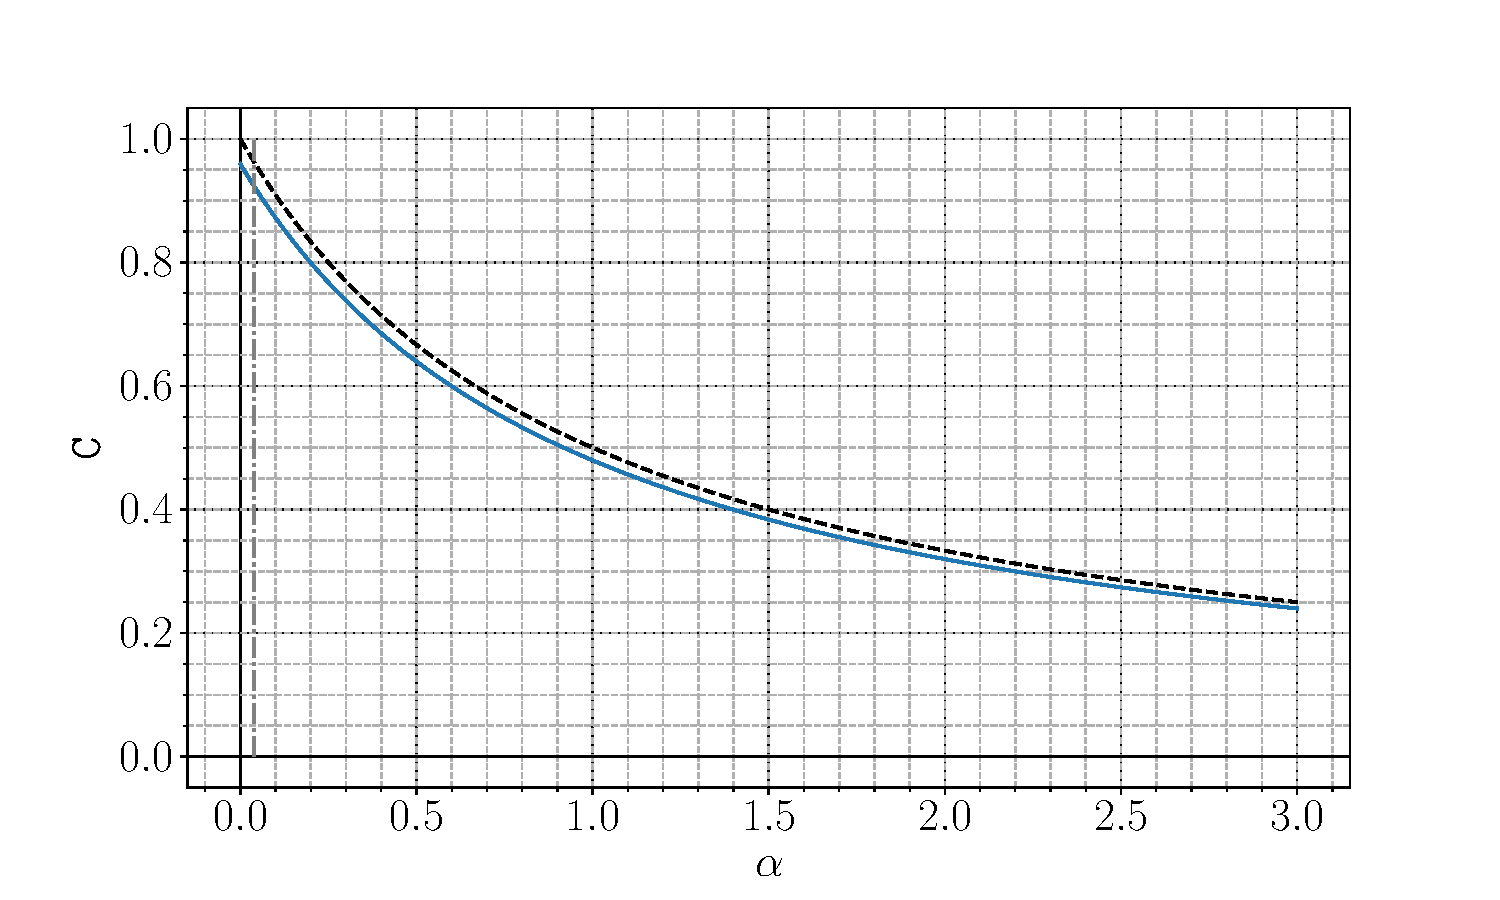
\includegraphics[width=0.7\textwidth]{contrast_bias}
  \caption[Interferometer contrast for an increasing
  resudual atoms ratio]{Interferometer contrast for an increasing
    residual atom ratio.
    The black dashed line indicates the reduction expected when no
    atoms are lost from \(\ket{F=2}\). The dot-dashed line indicates
  the ratio at which the loss in contrast from the residual atom
number dominates over the depopulation.}
  \label{fig:contrast_bias}
\end{figure}

\subsection{Estimating the Interferometer Phase}
The interferometer phase \(\Phi\) is determined from \EquationRef{eq:prob_measurement} using
\begin{equation}
\text{P}_{\ket{F=2}} = \text{P}_0+\frac{C}{2}\cos(\Phi)
  \label{eq:interferometer_phase}
\end{equation}
where P\(_0\) is the mean probability of detecting atoms in
\(\ket{F=2}\) and \(C\) is the interferometer fringe contrast.

\subsection{Sources of Detection Noise}\label{subsec:detection_noise}

Each measurement of the number of atoms has an uncertainty due to
random processes that influence the voltage measured by the detector. These errors
combine to give an uncertainty in the interferometer phase and
hence, acceleration. It is worth distinguishing between the different
sources of noise in measuring the number of atoms. Uncertainties due
to fluctuations in the number of atoms and detected photons per
measurement cannot be reduced below their shot-noise levels. In
particular, the phase noise corresponding to the atom shot noise is
the minimum value attainable. Therefore, it is essential that the
photo-detector used is sensitive enough to ensure that this does not
limit the sensitivity.
\subsubsection{Atom and Photon Shot Noise}
The discrete nature and the fact that atoms are loaded into the
experiment and scatter photons at a constant rate mean that the
statistics on the number of atoms and photons are well-described by
Poisson distributions. It follows that the number of atoms in the
interferometer as well as the number of photons arriving at the detector during
each measurement have
shot noise fluctuations. From~\EquationRef{eq:pd_signal}, these are related to an
equivalent output voltage as follows
\begin{align}
  \sigma_\text{at,v}^2 &= \alpha^2 \eta^2 R_\text{sc}^2 n_\text{at}\\
  \sigma_\text{p,v}^2 &= \alpha^2 \eta R_\text{sc} n_\text{at} 
  \label{eq:atom_photon_noise}
\end{align}
where \(\sigma_\text{at,v}\) dominates, provided at least one photon
per atom is detected. Hereafter, no attention will be paid to the
photon shot noise. For the detection parameters previously defined,
the shot noise is equal to around \sivalue{46.5}{\nano\volt} per atom. 
\par\noindent
In order for the uncertainty in the atom number to
be dominated by the atom shot noise, the detector must be sensitive
enough that it has a \ac{nep} much lower than the noise in the optical
power detected. The \ac{nep} of a detector is defined as the
equivalent optical power which gives a signal-to-noise ratio of 0
after an integration time of \sivalue{0.5}{\second}. It is convenient
to express this as a voltage density, by multiplying it by the
photodiode gain. Hence, the
voltage density of a detector whose sensitivity is at the atom shot noise
level for an integration time \(tau_D\) is given by
\begin{equation}
  V_\text{at} = \frac{\sigma_\text{at,v}}{\sqrt{1/2\tau_D}}
  \label{eq:nep}
\end{equation}. 

%In the time domain, the signal is convolved with a rectangular pulse
%of a characteristic time \(\tau\), so the power spectral density is a
%product of the individual power spectral densities
%\begin{equation}
%  S(f) = 2 S_0\left(\frac{\sin(\pi f \tau)}{\pi f \tau}\right)^2
%  \label{eq:psd_shot_conf}
%\end{equation}
%where \(S_0\) is the one-sided power spectral density of the shot
%noise component. From the Wiener-Khinchin theorem, the variance is
%equal to the integral of the power spectral density, so
%\begin{equation}
%  S_0 = \sigma^2_\text{i,v} \tau
%  \label{eq:shot_noise_amp}
%\end{equation}
%For shorter detection times, this has the effect of aliasing
%high-frequency noise into the lower-frequency components.  
%The number of photons
%arriving at the detector in a time interval \(\Delta t\) is given by
%\begin{align}
%  n_p &= N R_\text{sc}(I,\Delta) \eta \delta t \nonumber\\
%  &= \alpha N
%  \label{eq:photon_detector}
%\end{align}
%where \(\eta\) is the collection efficiency of the detector, \(N\) is
%the number of atoms and \(R_\text{sc}\) is the scattering rate defined
%in \EquationRef{eq:scattering_rate}. The atom shot noise and photon
%shot noise are given by \(\sigma_N = \sqrt{N}\) and \(\sigma_p =
%\sqrt{n_p}\), respectively. The
%uncertainty in the number of detected photons \(\sigma_D\) has
%contributions from both the atom shot noise and the photon shot noise
%\begin{equation}
%  \sigma_D = \sqrt{\alpha^2\sigma_N^2 + \sigma_p^2} 
%  \label{eq:detection_uncertainty}
%\end{equation}
%This is dominated by the atom shot noise when \(\alpha^2 > 1\), i.e. when
%more than one photon per atom is detected by the photodiode. 
%\par\noindent
%There is additional contribution to \(\sigma_D\) from the technical
%noise of the detector. The signal from the photodiode is averaged over
%the detection time \(\Delta t\), so the variance in this is given by
%\begin{equation}
%  \sigma_v = \int_0^{f_c} |S_\text{pd}|^2 \mathrm{d}f 
%  \label{eq:photodiode_noise_bandwidth}
%\end{equation}
%where \(|S_\text{pd}|^2\) is the one-sided power spectral density of the
%photodiode signal and \(f_c = 1/(2\Delta t)\) is the frequency
%bandwidth.   
\subsubsection{Photodiode Technical Noise}
Technical noise in the detector typically arises from multiple electronic processes -- such as Johnson noise and shot noise in
the current -- but it is not necessary to consider them independently
in the following discussion. The technical noise of the detector can
be estimated by measuring the output voltage when no light is
collected. A plot of the power spectral density of the photodiode is shown in~\FigureRef{fig:pd_psd} taken
with a sampling frequency of \sivalue{200}{\kilo\hertz}. The
photodiode was covered and the output voltage was sampled for
\sivalue{2}{\second}. The power spectral density has been calculated
using Welch's method~\cite{Welch1967}. The data are partitioned before
calculating the Fourier transform of each subset and taking the
average. This has the effect of reducing the variance in the estimated
power spectrum at the expense of reducing the frequency resolution.
Below \sivalue{10}{\kilo\hertz} the power spectral density is close
to uniform with a value of around
\sivalue{5e-13}{\volt\squared\per\hertz}, which corresponds to a
noise-equivalent power of \sivalue{391}{\femto\W\per\hertz\tothe{1/2}}.
For higher frequencies, the power spectral density starts to
increase. The plot also indicates the corresponding voltage noise
density to reach the
atom shot noise limit for atom numbers of 
of n\(_\text{at} =\) \num{5e6} and \num{1e6} with the previously
defined output voltage per atom. 
\begin{figure}[htpb!]
  \centering
  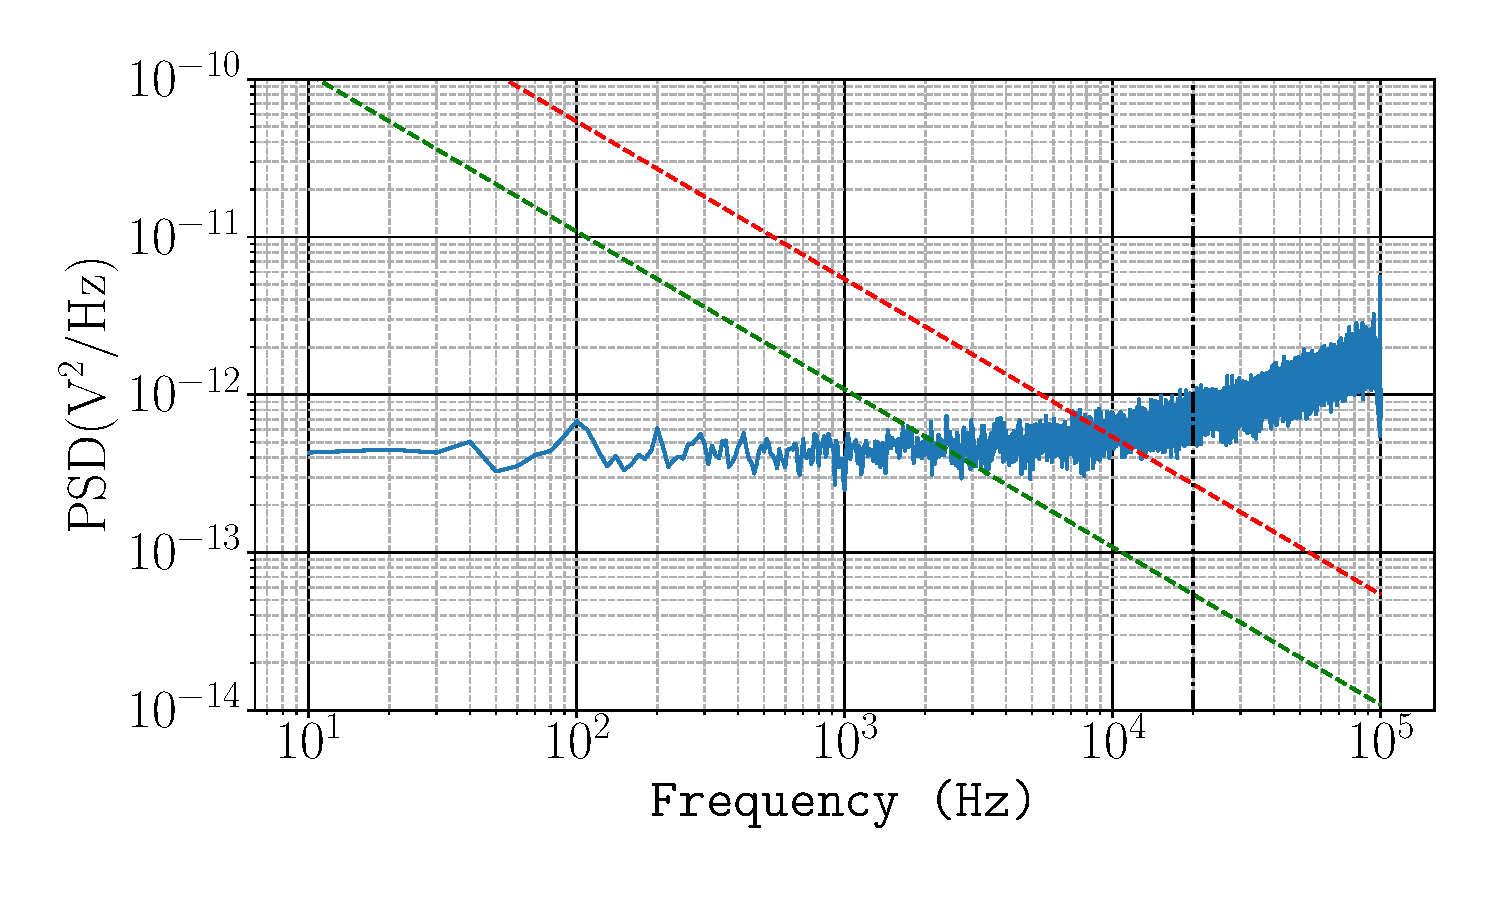
\includegraphics[width=0.7\textwidth]{noise_source_psd}
  \caption[Photodiode power spectral density]{Power spectral density of the photodiode output voltage
  sampled for \sivalue{2}{\second} at a rate of
\sivalue{200}{\kilo\hertz}. The red and green dashed lines indicate
the required voltage noise density to equal the atom shot noise level
after integrating for \(\tau = 2/f\)\sivalue{}{\s} for atom numbers of
\num{5e6} and \num{1e6}, respectively.}
  \label{fig:noise_source_psd}
\end{figure}
Averaging the detection signal over a time \(\tau\) has the effect of
filtering the signal above the Nyquist frequency \(f_n = 1/(2 \tau)\).
The variance in the averaged voltage over successive shots
i.e. the Allan variance, is related to the power spectral density as
follows
\begin{equation}
  \sigma^2_\text{av}(\tau) = 2 \int_0^\infty \frac{\sin(\pi \tau f)^4}{(\pi \tau f)^2}S(f)\;\mathrm{d}\;f
  \label{eq:av_psd}
\end{equation}
Using~\EquationRef{eq:av_psd}, it is possible to determine the
detection time required to reduce the shot-to-shot variance below the
atom shot noise level. A plot of the Allan deviation for increasing
integration time is shown
in~\FigureRef{fig:detection_av}, along with the rms voltage expected
for the same numbers of atoms used
in~\FigureRef{fig:noise_source_psd}. At the integration time of
\sivalue{200}{\micro\second}, the detector noise
is close to \sivalue{5}{\micro\volt} -- well below the level of the
atom shot noise.
\begin{figure}[htpb!]
  \centering
  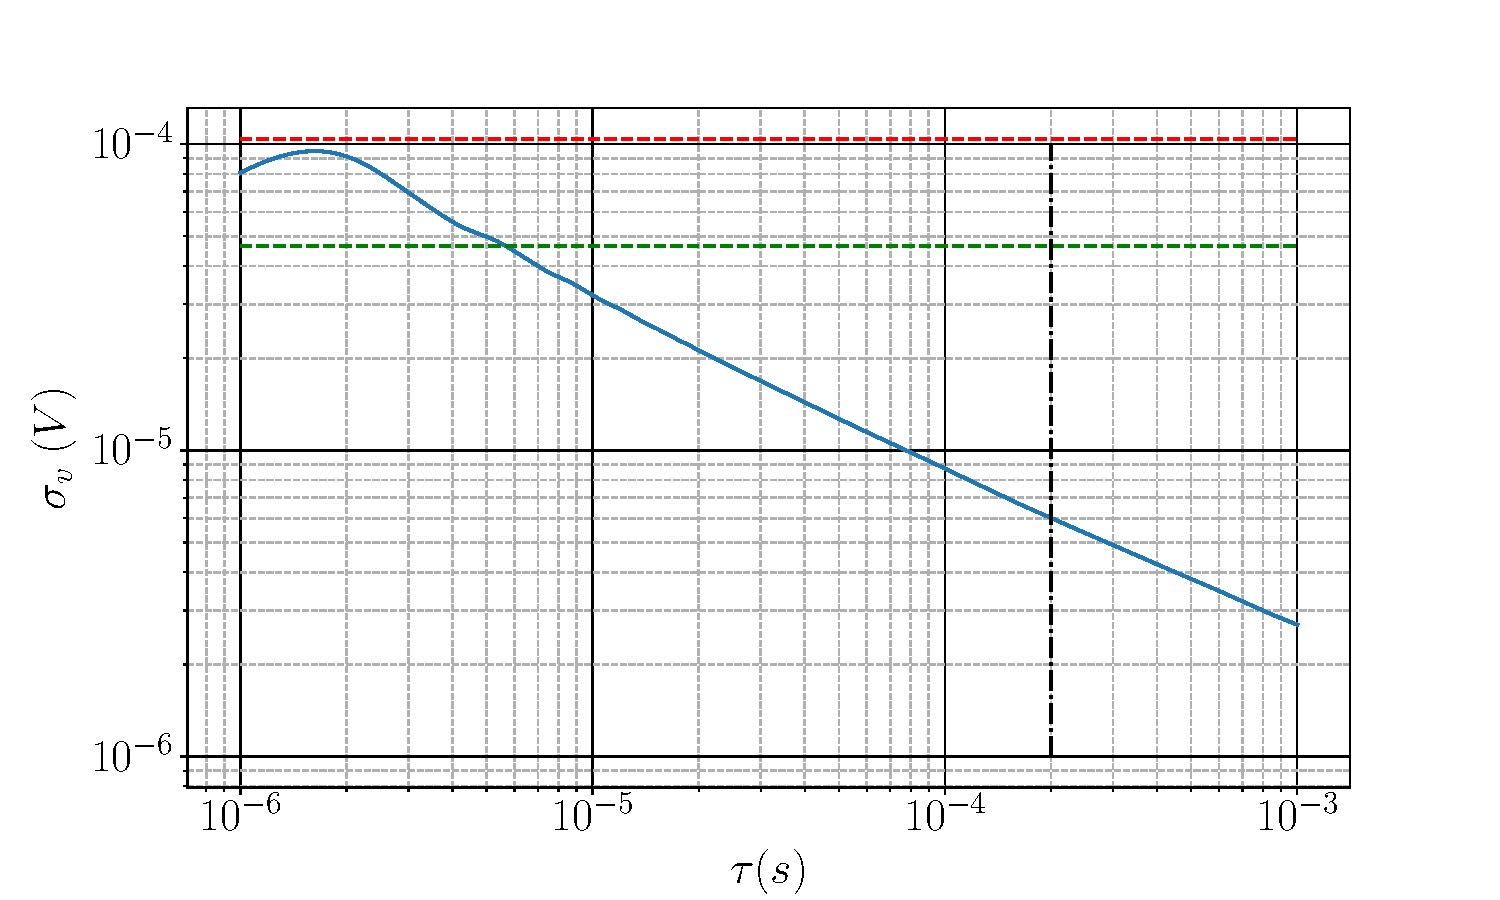
\includegraphics[width=0.5\textwidth]{detection_av}
  \caption{Allan variance of the Photodiode voltage for increasing
  integration time \(\tau\). The red and green dashed lines are the
atom shot noise rms voltages for the values used
in~\FigureRef{fig:noise_source_psd}. The black dot-dashed line indicates the
integration time of \sivalue{200}{\micro\second} used in the
experiment.}
  \label{fig:detecion_av}
\end{figure}

\section{Individual Pulse Characterisation} \label{sec:atomint_rabiosc}
This section presents a characterisation of the pulses used to drive
Raman transitions between the two hyperfine ground states. First, the
properties of the Raman transition spectrum are presented
in~\SectionRef{subsec:raman_spec}. Following this, a discussion of
cancelling the systematic phase from a differential ac Stark Shift is
given in~\SectionRef{subsec:light_shift}. Finally, this section
concludes with specific details about the individual pulses used in
the experiment. The first Raman pulse, which is used to select a
subset of atoms with a narrow velocity spread, is presented
in~\SectionRef{subsec:vel_select}. This is followed by a presentation
of the dynamics of the three pulses used to coherently control the
atoms during the interferometer in~\SectionRef{subsec:int_pulses}
\subsection{Raman Transition Spectrum}\label{subsec:raman_spec}

\begin{itemize}
	\item Raman transition spectrum identifying Doppler width
	\item Explain the large co-propagating peak
	\item Asymmetry between \(\pm k\)
\end{itemize}
During the state preparation sequence, the majority of the atoms are
optically pumped into the \(\ket{1,0}\) state. Ideally, each
Raman beam is perfectly circularly polarised and can only drive
\(\ket{1,0}\leftrightarrow\ket{2,0}\) transitions using either of the
counter-propagating pairs of beams. More generally, the selection
rules of the Raman transition allow for transitions between other
states, depending on the polarisation of the light. The allowed
transitions between the different Zeeman states are presented
in~\TableRef{tab:raman_trans}. The laser polarisation
configurations are given in~\TableRef{tab:raman_pol_config}. These
are defined for an atom being excited from \(\ket{F=1}\) and
stimulated into \(\ket{F=2}\), so that the \(\vec{k}_2\) beam
\textit{decreases} the angular momentum when it drives a \(\sigma^+\)
transition. 
\par\noindent
An example of the Raman transition spectrum
is shown in~\FigureRef{fig:raman_spectrum}. This beat frequency
between the two Raman lasers is scanned and a pulse is applied for
\sivalue{160}{\micro\second} to drive atoms into the \(\ket{F=2}\)
state. There is a large peak close to the hyperfine splitting
frequency. This peak is a result of Doppler-insensitive co-propagating
transitions\footnote{When the two light fields are co-propagating, the
  Doppler resonance term \(\delta_\text{D} \propto \vec{k}_1 -
\vec{k}_2\) is close to zero}. This indicates that the two Raman beams
are not orthogonally polarised, as that cannot drive co-propagating
transitions. This is further supported by the fact
that there are \(\Delta m = \pm 1\) transitions, which can only occur
if one of the lasers drives a \(\pi\) transition. The Zeeman shift on
the co-propagating transitions between \(\ket{F=1,0}
\rightarrow \ket{F=2,1}\) and \(\ket{F=1,1}\rightarrow \ket{F=2,1}\)
are \sivalue{95}{\kilo\hertz} and \sivalue{189.5}{\kilo\hertz}, which
correspond to a bias field of \sivalue{1.35}{\gauss}.
\begin{table}
  \centering
  \begin{tabular}{ccccc}
    \toprule
    & & \multicolumn{3}{c}{\(\vec{k}_2\)} \\
     \midrule
     & & \(\sigma^-\) & \(\pi\) & \(\sigma^+\)\\
     \multirow{3}{*}{\(\vec{k}_1\)} & \(\sigma^-\) &  c\(_1\) &
     c\(_2\)&
     --  \\
     & \(\pi\) &c\(_3\) & -- & c\(_4\) \\
     & \(\sigma^+\) & --& c\(_5\)& c\(_6\)\\
    \bottomrule
  \end{tabular}
  \caption[Raman transition polarisation configurations]{Labels for Raman transitions excited
    from \(\ket{F=1}\) by \(\vec{k}_1\) and stimulated into
  \(\ket{F=2}\) by \(\vec{k}_2\).}
  \label{tab:raman_pol_config}
\end{table}
\begin{table}
  \centering
  \begin{tabular}{ccccccc}
    \toprule
     & & \multicolumn{5}{c}{\(\ket{F=2,m}\)} \\
     \midrule
     & & -2 & -1 & 0 & 1 & 2 \\
     \multirow{3}{*}{\(\ket{F=1,m}\)} & -1 & (c\(_2\),c\(_4\)) &
     (c\(_1\),c\(_6\)) &(c\(_3\),c\(_6\))& -- & --  \\
     & 0 & & (c\(_2\),c\(_4\))& (c\(_1\),c\(_6\)) & (c\(_3\),c\(_6\))
     &-- \\
     & 1 & --& --&(c\(_2\),c\(_4\))& (c\(_1\),c\(_6\)) & (c\(_3\),c\(_6\)) \\
    \bottomrule
  \end{tabular}
  \caption{Allowed polarisation configurations between each hyperfine
  ground state Zeeman sub-levels.}
  \label{tab:raman_trans}
\end{table}
\begin{figure}[htpb]
  \centering
  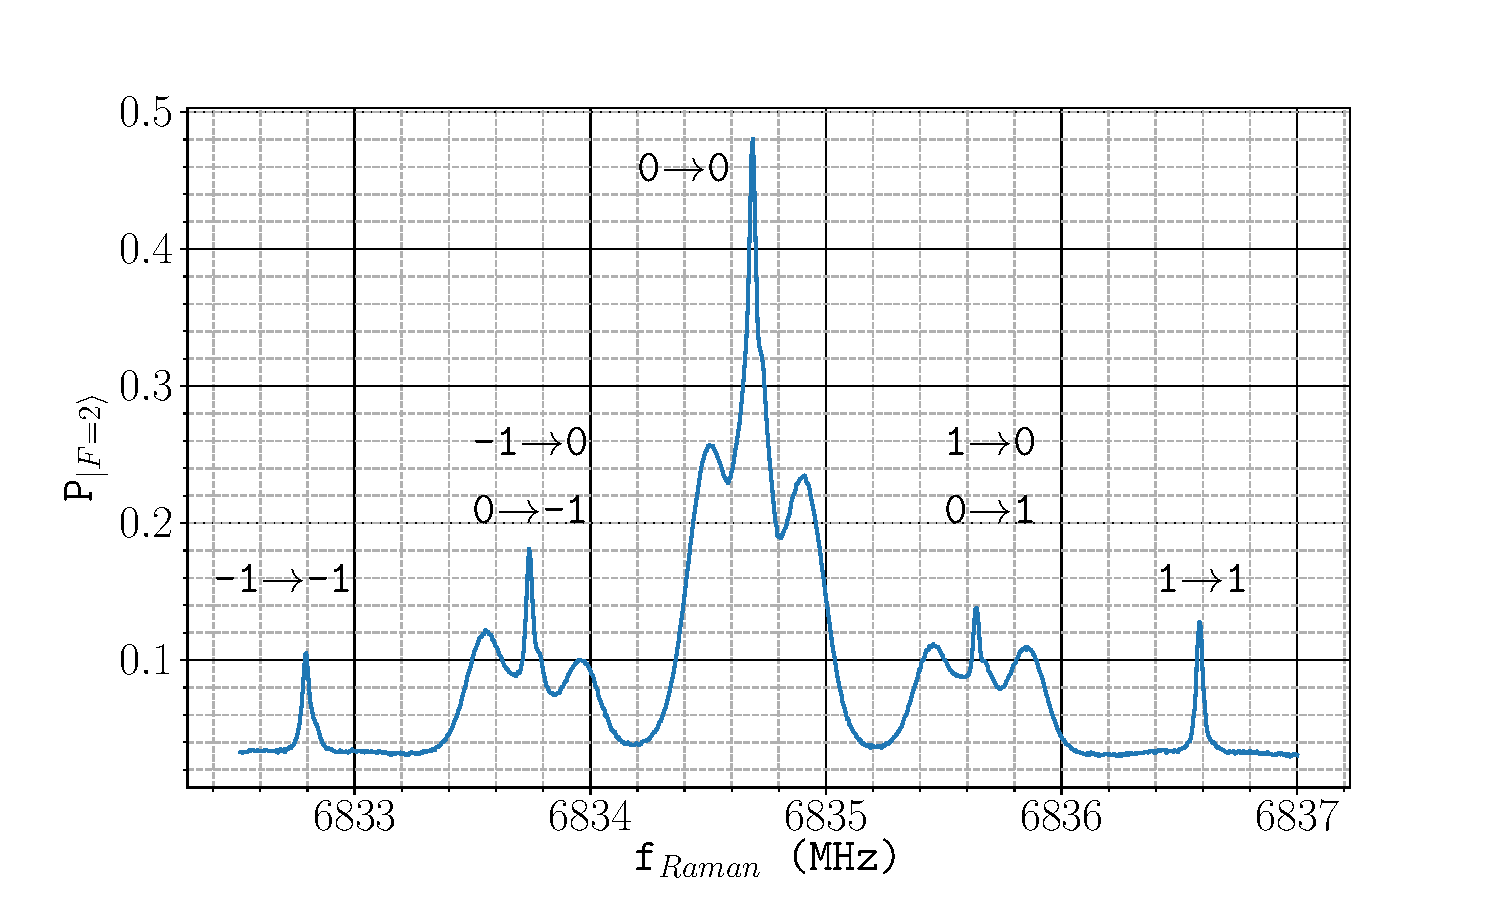
\includegraphics[width=0.5\textwidth]{raman_spectrum}
  \caption[Raman transition spectrum]{Raman transition spectrum, obtained by scanning the beat
    frequency of the two Raman lasers. The transitions \(\ket{1,m_F}
  \rightarrow \ket{2,m_F'}\) are indicated at each observed peak.}
  \label{fig:raman_spectrum}
\end{figure}
\par\noindent
Each co-propagating transition from \(\ket{1,0}\) has two smaller
peaks which are the Doppler-sensitive counter-propagating transitions.
The central peak is shown in more detail
in~\FigureRef{fig:raman_spectrum_inset}. The counter-propagating
transitions are shifted by \sivalue{-185}{\kilo\hertz} and
\(+\)\sivalue{215}{\kilo\hertz} respectively, which correspond to
velocities of \sivalue{7.2}{\centi\metre\per\second} and
\sivalue{8.4}{\centi\metre\per\second}. The same Doppler shifts are also
observed in the peaks corresponding to the \(\ket{F=1,m_F = 0}
\rightarrow \ket{F=2,m_F=\pm 1}\) transitions. The counter-propagating transitions are
Doppler-broadened by the thermal velocity of the atoms along the direction
of the Raman beams. Fitting the transition to the lineshape expected
from a thermal distribution of atoms gives a temperature of
\sivalue{15}{\micro\kelvin} and \sivalue{13.5}{\micro\kelvin} from
each counter-propagating transition. At the time this spectrum was
measured, the molasses was not optimised to give the lowest
temperature.
\begin{figure}[htpb!]
  \centering
  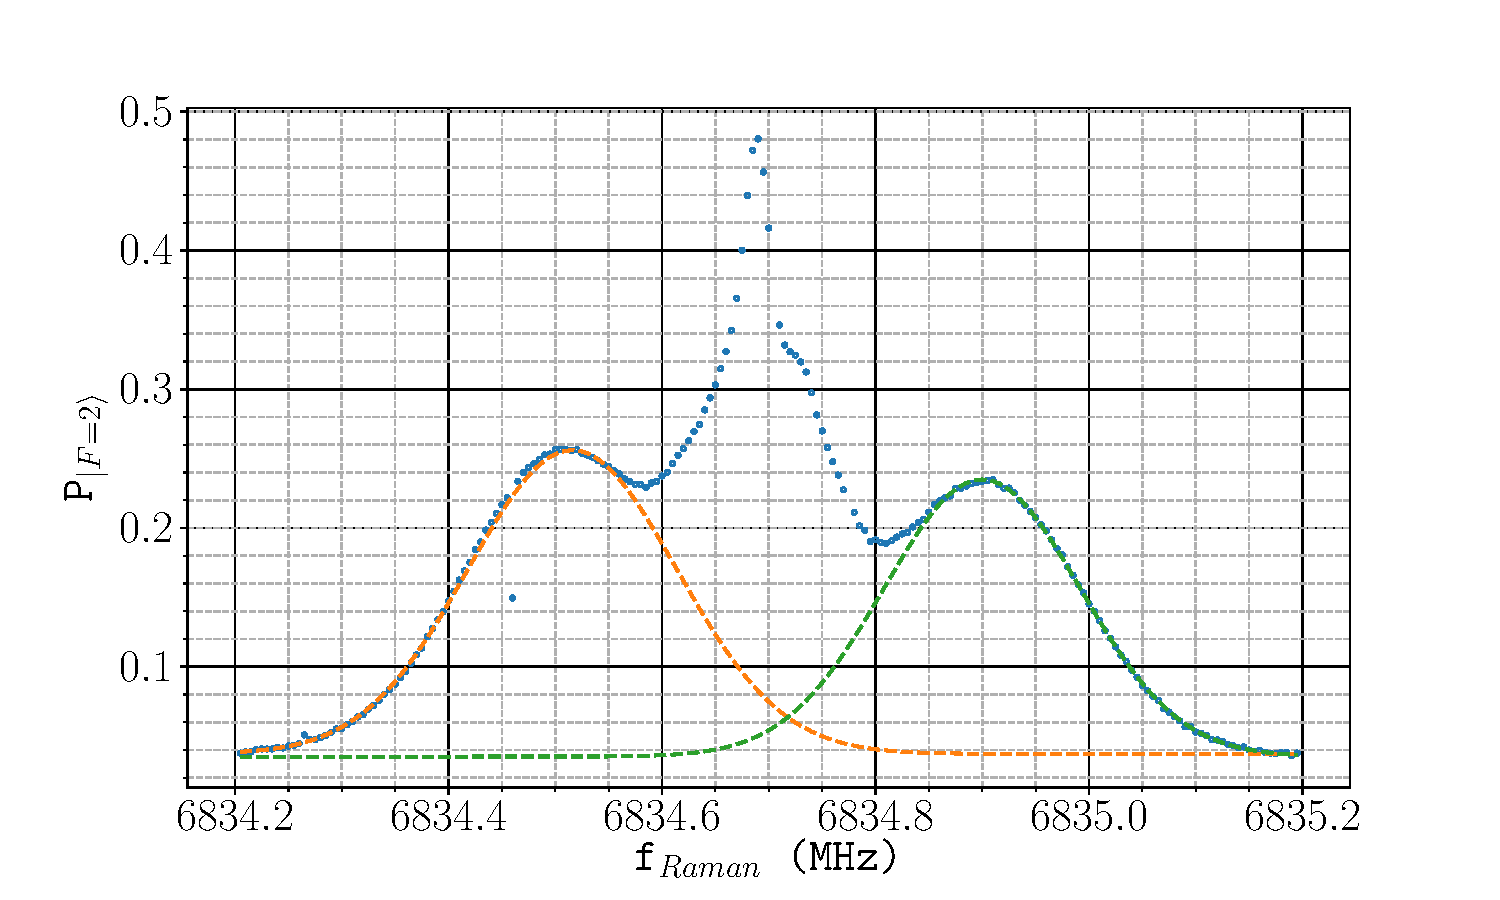
\includegraphics[width=0.5\textwidth]{raman_spectrum_inset}
  \caption[\(\Delta m = 0\) transition spectrum.]{Transition spectrum showing the \(\Delta m = 0\) transition
  from \(\ket{1,0}\). The orange and green dashed lines are fits to a
Doppler-broadened lineshape for each of the counter-propagating
profiles.}
  \label{fig:raman_spectrum_inset}
\end{figure}
\subsection{Cancelling the Differential ac Stark
Shift}\label{subsec:light_shift}
It is worth considering the effects of ac Stark shifts on an atom
interferometer atom interferometer. Firstly, they are intrinsically related to the
effective Rabi frequency and as such, cannot be avoided. The average
ac Stark shift \(\Omega^\text{ac}_\text{avg} = (\Omega_1^\text{ac} +
\Omega_2^\text{ac})/2 \) (see~\SectionRef{sec:raman_trans_theory}) is
the same along both paths of the interferometer, provided that the
intensity variation of the Raman beams over the path separation can be
neglected. Therefore, this should not lead to an observable phase
shift.
\par\noindent
On the other hand, the differential ac Stark shift \(\delta^\text{ac}
= \Omega_1^\text{ac} - \Omega_2^\text{ac}\) can lead to an observable
phase shift. Using the results from Ref.~\cite{Weiss1994} for \(\pi\)
and \(\frac{\pi}{2}\) pulses, the phase shift to a Mach-Zender type
interferometer is
\begin{equation}
  \Delta \phi^\text{ac} =
  \frac{\delta_3^\text{ac}}{\Omega_\text{eff}} - \frac{\delta_1^\text{ac}}{\Omega_\text{eff}} 
 \label{eq:diff_phase}
\end{equation}
where \(\delta_3^\text{ac}\) and \(\delta_1^\text{ac}\) are the ac
Stark shifts of the last and first \(\frac{\pi}{2}\) pulses,
respectively. Therefore, the interferometer is sensitive to the
difference in the ac Stark shift of these pulses. 
\par\noindent
As the atoms fall
under gravity, it is likely that the intensity of the Raman beams
during these pulses will not be the same. Fortunately, it is possible
to eliminate this differential phase shift using an appropriate choice
of intensity and detuning of the Raman lasers. This can be seen by
first writing out the differential ac Stark shift
\begin{equation}
  \delta^\text{ac} = \Omega_1^\text{ac} - \Omega_2^\text{ac} = \sum{ik}
  \frac{\lvert\Omega_{1ik}\rvert^2}{4\Delta_{1ik}} - \sum{ik}
  \frac{\lvert\Omega_{2ik}\rvert^2}{4\Delta_{2ik}} 
  \label{eq:diff_shift}
\end{equation}
in terms of the one-photon Rabi frequencies \(\Omega_{1ik}\) and
detunings \(\Delta_{1ik}\). When both Raman beams are red-detuned from
all the one-photon transitions, both terms
in~\EquationRef{eq:diff_shift} are strictly negative. Therefore,
\(\delta^\text{ac}\) can be cancelled by choosing the correct
intensities for each Raman beam. A plot of \(\delta^{\text{ac}}\)
for various Raman beam intensities as a function of the ratio between
the two Raman beams is shown in~\FigureRef{fig:light_shift_ratio}. There
is a ratio at which the differential ac Stark shift cancels and is
independent of the total intensity. The ratio that cancels
\(\delta^\text{ac}\) for increasing two-photon detuning \(\Delta_R\) is shown
in~\FigureRef{fig:light_shift_detuning}. When \(\Delta_R\) is
\sivalue{-1.13}{\giga\hertz} below the \trans{2}{3} transition, this
ratio is maximised. The differential ac Stark shift is cancelled when
the intensity ratio of light driving \(\ket{1,0}\) transitions to
\(\ket{2,0}\) transitions is \(\mathcal{R} = 0.583\). 
\begin{figure}[!htbp]
	\centering
	\def\svgwidth{\columnwidth}
	\subfloat[][]{\scalebox{0.3}{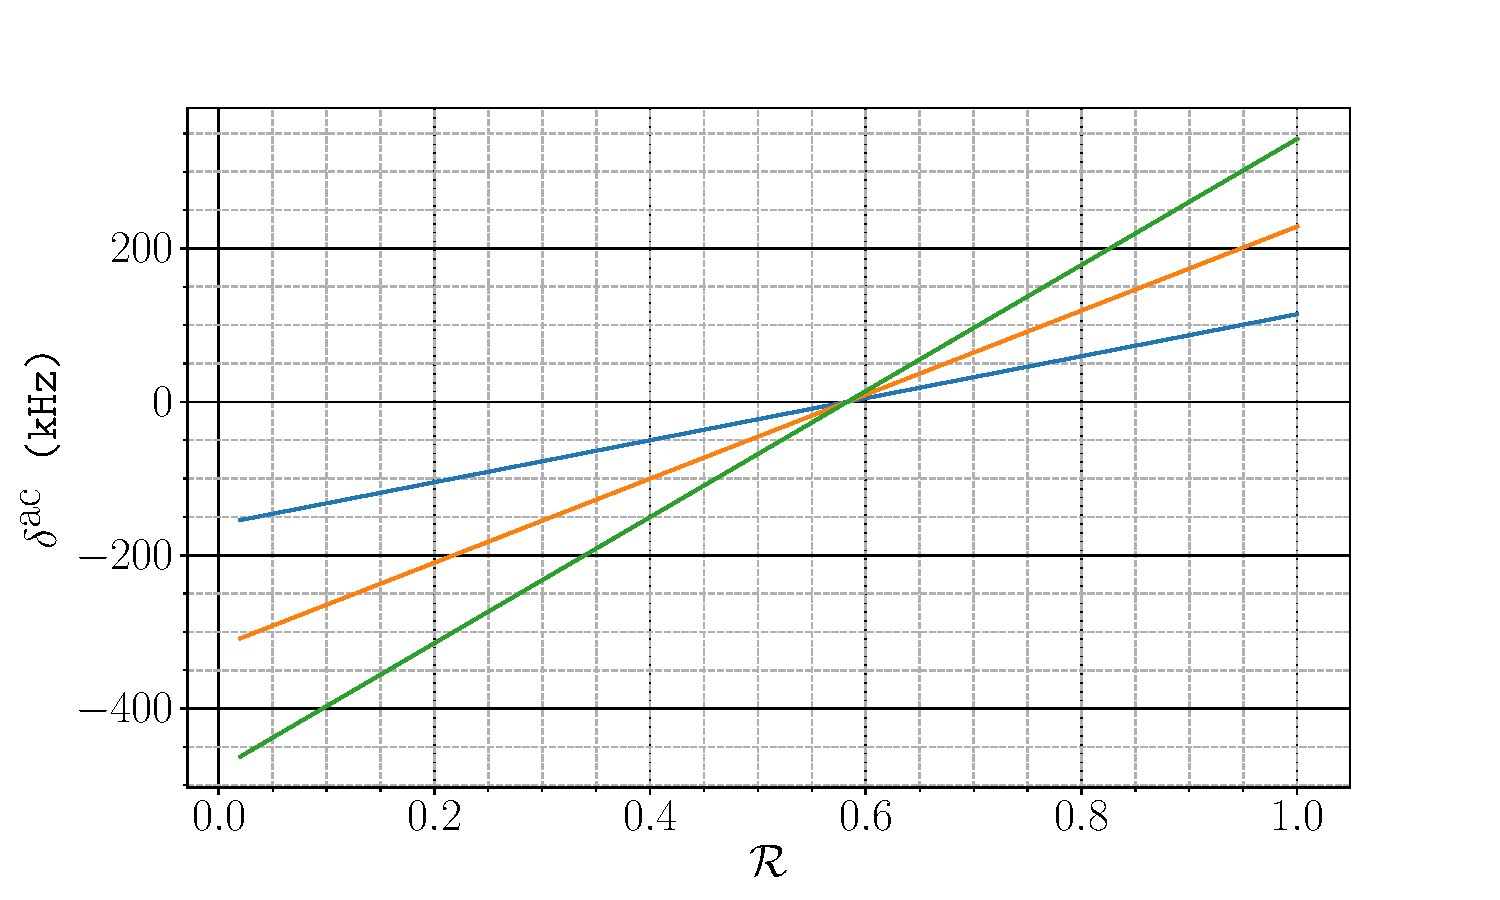
\includegraphics{light_shift_ratio}}\label{fig:light_shift_ratio}}
\subfloat[][]{\scalebox{0.3}{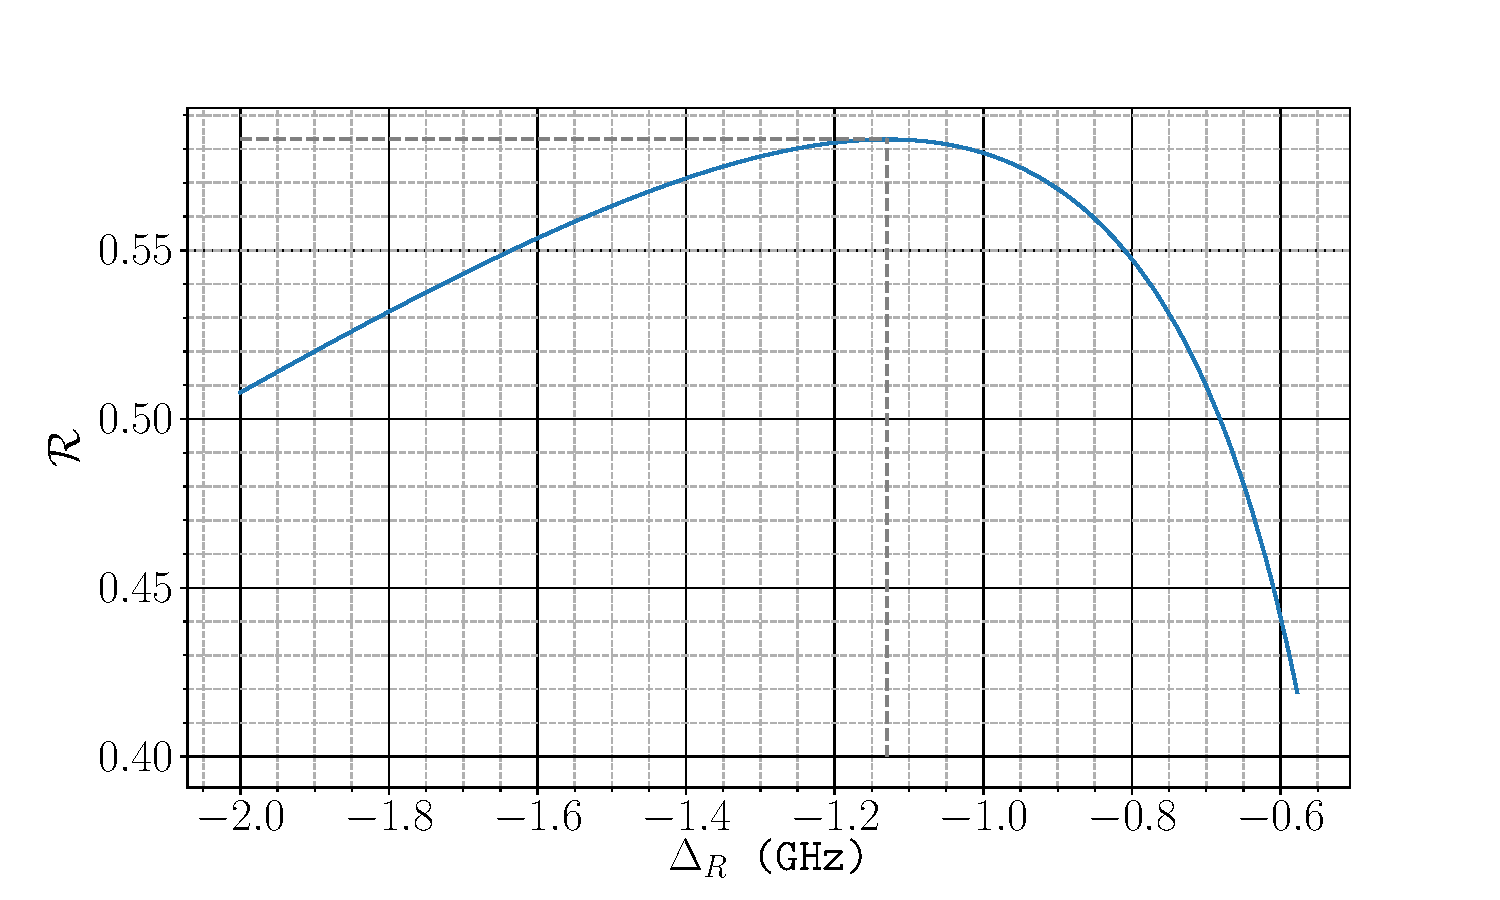
\includegraphics{light_shift_detuning}}\label{fig:light_shift_detuning}}\\
	\caption[Differential ac Stark shift as a function of two-photon
  detuning and Raman beam intensities]{The effects of the Raman beam
  intensities and detuning on the differential ac Stark shift
  \(\delta^\text{ac}\).
\textbf{(a)} shows \(\delta^\text{ac}\) as a function of the intensity ratio
\(\mathcal{R}\) between the light which drives transitions from
\(\ket{1,0}\) to the light that couples to \(\ket{2,0}\) for the
two-photon detuning of \(\Delta_R = -\sivalue{1.13}{\giga\hertz}\)
used in the experiment. Example
intensities for the \(\ket{2,0}\) light are
\sivalue{100}{\watt\per\metre\squared} (blue),
\sivalue{200}{\watt\per\metre\squared} (orange) and
\sivalue{300}{\watt\per\metre\squared} (green). \textbf{(b)} shows how
the ratio for which \(\delta^\text{ac} = 0\) varies as \(\Delta_R\)
increases. The dashed lines indicate the value of \(\Delta_R\) used in
the experiment and its corresponding ratio of 0.583.}
	\label{fig:light_shift_plots}
\end{figure}
\par\noindent
Since it is not straight-forward to directly measure the intensity of
each Raman beam on the atoms, a better method to cancel the
differential ac Stark shift is to use the transition spectrum to
determine when the intensity of the lasers are set to the appropriate
ratio. Experimentally, this was done by adjusting the power of the
pump lasers for the master and slave Solstis lasers. When the master
is seeded with \sivalue{10}{\watt} and the slave with
\sivalue{6.5}{\watt}, the differential ac Stark shift is eliminated.
\FigureRef{fig:cancelled_light_shift} shows the transition spectrum using two different effective Rabi
frequencies, corresponding to \(\pi\) pulse times of
\sivalue{22.5}{\micro\second} and
\sivalue{45}{\micro\second}. In this instance, the frequency difference of the two
co-propagating peaks is less than \sivalue{1}{\kilo\hertz}.
\begin{figure}[htpb!]
  \centering
  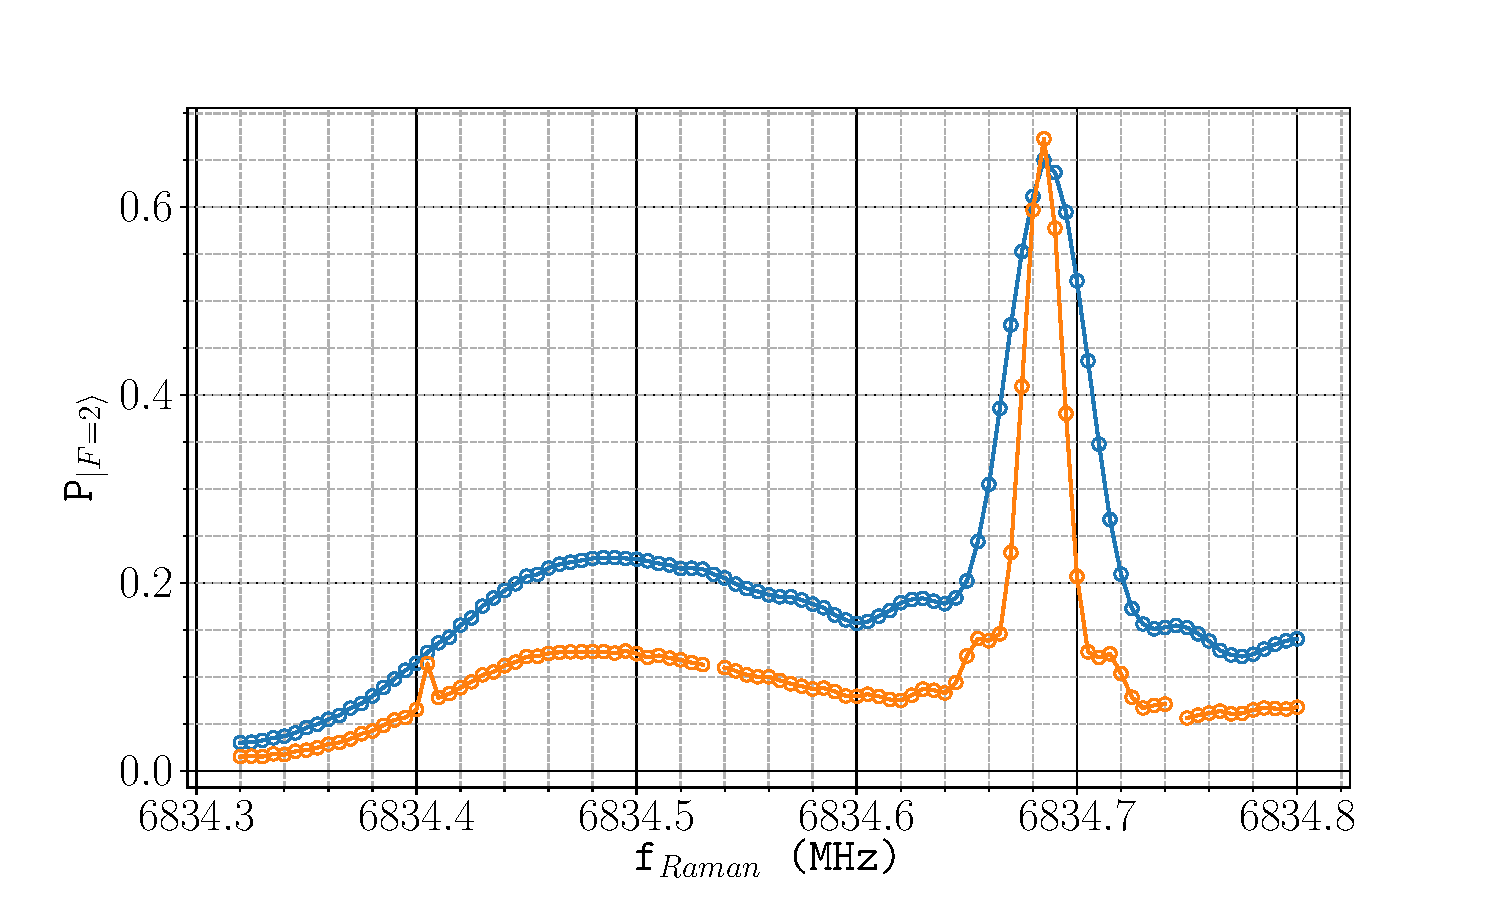
\includegraphics[width=0.5\textwidth]{cancelled_light_shift}
  \caption[Raman transition spectrum after cancelling the differential
  ac Stark shift.]{Raman transition spectrum after cancelling the differential
    ac Stark shift. The blue (orange) curve shows a pulse with a \(\pi\) pulse
  time of \sivalue{22.5}{\micro\second}
(\sivalue{45}{\micro\second}).}
  \label{fig:cancelled_light_shift}
\end{figure}
\(\Omega_2^\text{ac}\)
It is shifted by \sivalue{1.4}{\mega\hertz} from
\(f_\text{hfs}\). Since the differential light shift has been
cancelled (see \SectionRef{subsec:light_shift}), this is a result of a
second-order Zeeman shift and corresponds to a field strength of
\sivalue{1.56}{\gauss}.
\subsection{Velocity-Selective Pulse}\label{subsec:vel_select}
\begin{itemize}
	\item Spectrum after velocity selection
	\item How does linewidth of Raman pulse affect final velocity distribution?
	\item Why do we need this?
	\item How to explain the pulse-probe spectrum
\end{itemize}
Since the Raman transition is Doppler-sensitive, it is necessary to
consider the effects of the velocity spread of the atoms that are
present. At a temperature of \sivalue{6}{\micro\kelvin}, the Doppler
width is \(\sigma_f = \frac{2}{\lambda}\sqrt{\frac{k_b T}{m}}
\approx\) \sivalue{60}{\kilo\hertz}. Coherent control of the atomic
state during the interferometer requires that the linewidth of the Raman
transition must be much broader than the Doppler width. This ensures
that each atom is driven at approximately the same Rabi frequency,
reducing the dephasing rate of the atomic coherence. The linewidth of
a Raman transition is determined solely by the pulse intensity and
duration. A pulse duration of \sivalue{7}{\micro\second} has a
linewidth close
to the Doppler width, but the intensities required for this are above
what is attainable with our Raman laser. 
\par\noindent
It is possible to reduce the Doppler width of the participating atoms
by first applying a Raman pulse to select a subset of the population
with a narrower velocity spread~\cite{Moler1992}. In general, the velocity-selective pulse ought to have
a narrower linewidth than the subsequent ones. This ensures that the
Doppler width of atoms in the interferometer is small compared with
the Raman transition linewidth. Starting with a velocity distribution of atoms
described by a 1-D Maxwell-Boltzmann distribution all occupying the
\(\ket{1,0}\) state, the
population in \(\ket{2,0}\) after applying a Raman pulse is
distributed according to
\begin{equation}
  P_{\ket{2,0}}(v) = \frac{\Omega_R^2}{\Omega_R^2 + \delta^2}
  \sin\left(\sqrt{\Omega_R^2+\delta^2}\;\tau\right)^2 p(v)
  \label{eq:vel_selected_dist}
\end{equation}
where\(\delta\) is the Raman detuning defined
in~\EquationRef{eq:raman_detuning}, \(p(v) = \sqrt{\frac{m}{2\pi
k_B T}} e^{-\frac{m v^2}{2 k_B T}}\) is the velocity distribution and
\(\Omega_R\) is the effective Rabi frequency. A plot of the
distribution of atoms driven by a \(\pi\) pulse with a duration of
\sivalue{40}{\micro\second} and a temperature of
\sivalue{6}{\micro\kelvin} is shown
in~\FigureRef{fig:vel_selected_dist}, where the velocity is given in
units of frequency. The population that is stimulated
has a mean velocity shifted by twice the recoil velocity. In this
instance, the rms
frequency is \(\sigma_f
=\)\sivalue{19.7}{\kilo\hertz}.
\begin{figure}[htpb!]
  \centering
  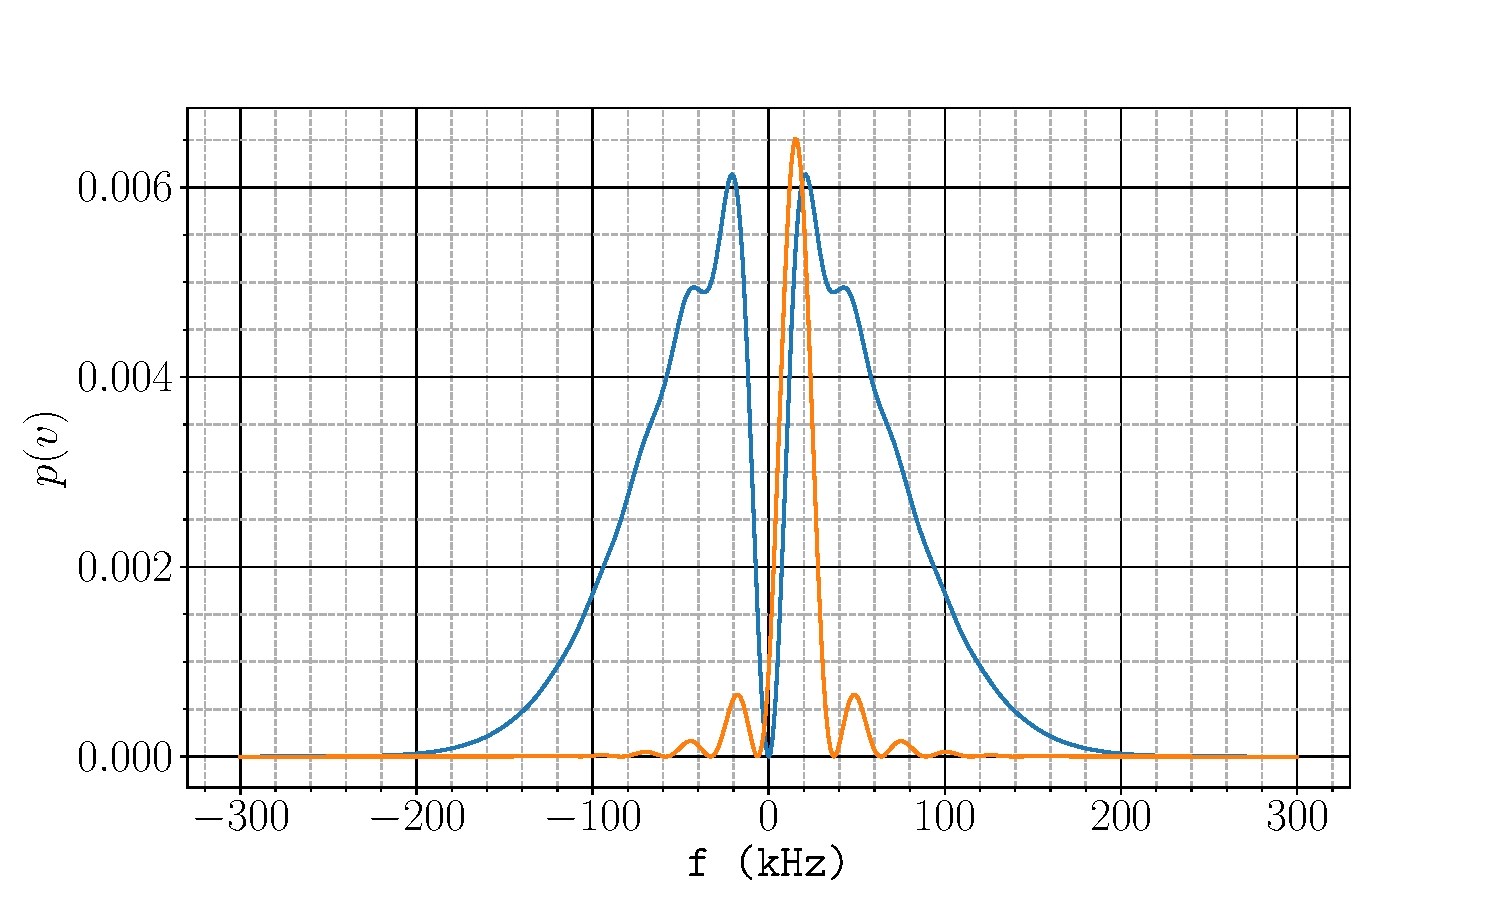
\includegraphics[width=0.5\textwidth]{vel_selected_dist.pdf}
  \caption{Velocity distribution of a \sivalue{6}{\micro\kelvin}
  ensemble of atoms after a \sivalue{40}{\micro\second} Raman \(\pi\)
pulse. The mean velocity of the stimulated distribution, shown in
orange, is increased due to the recoil during the transition.}
  \label{fig:vel_selected_dist}
\end{figure}
\subsubsection{Velocity-Selected Distribution}
The velocity distribution of atoms after the velocity selective pulse
can be measured using a second Raman pulse as a probe. In contrast to
the interferometer pulses, this probe must be much lower power than
the velocity-selective pulse so that its linewidth is comparatively narrow.
A measurement of the velocity distribution of the atoms is shown
in~\FigureRef{fig:vel_select_chirp}. An initial
\sivalue{40}{\micro\second} \(\pi\) pulse with a Raman beat frequency
\(f_v = \) \sivalue{6834.51}{\mega\hertz} prepares atoms in
\(\ket{1,0}\), before blowing away the atoms which remain in
\(\ket{F=2}\). After \sivalue{10}{\milli\second}, a
\sivalue{80}{\micro\second} \(\pi\) pulse transfers some of the
remaining population back into \(\ket{2,0}\). The frequency of the
probe pulse is varied by chirping the Raman laser beat frequency. In
this instance, the power of the pulse was not tuned to give a \(\pi\)
pulse area so the measured population is not indicative of the maximum
driven by the Raman transition. It is clear that the velocity
distribution of the selected atoms is narrower than the initial
thermal distribution. Fitting to a 1D Maxwell-Boltzmann distribution
gives an effective temperature of around \sivalue{1}{\micro\K}.
\begin{figure}[htpb!]
  \centering
  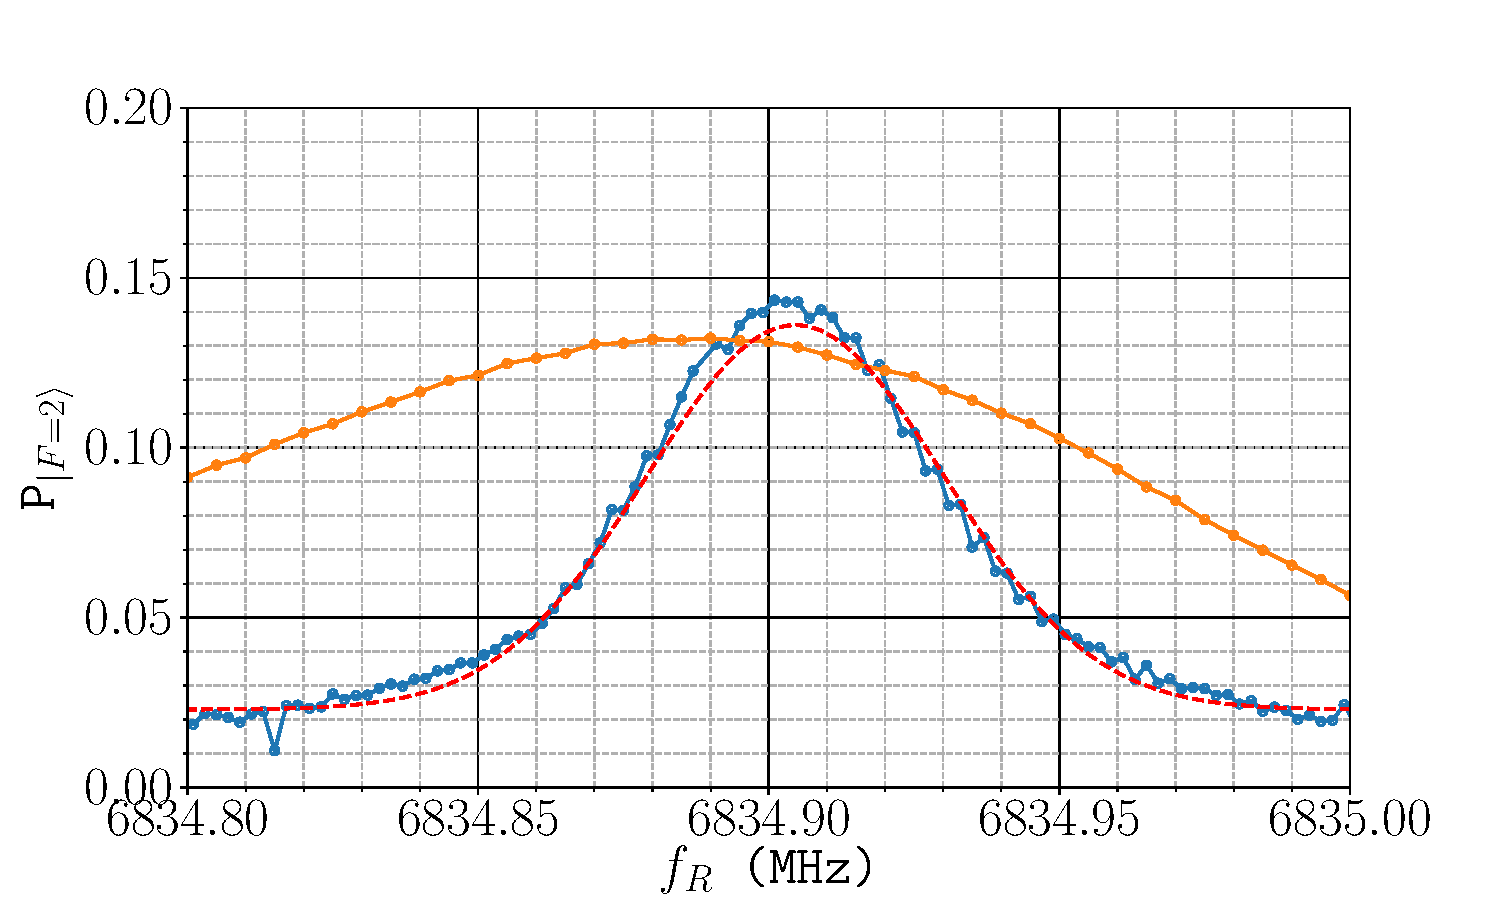
\includegraphics[width=0.6\textwidth]{RamanChirp.pdf}
  \caption{\(\ket{F=2}\) population after a Raman pulse at a frequency
    \(f_v =\)\sivalue{6834.51}{\mega\hertz} transfers atoms to
    \(\ket{1,0}\). This distribution is probed by
  applying a narrow pulse at a frequency \(f_{R}\). The population
measured in \(\ket{F=2}\) is shown in blue. The red dashed line is a
fit to a 1D Maxwell-Boltzmann distribution of the Doppler-broadened
transition peak. For comparison, the
transition spectrum of a single \(\tau = \)\sivalue{40}{\micro\s} \(\pi\)
pulse is shown in orange.}
  \label{fig:vel_select_chirp}
\end{figure}
\subsection{Interferometer Pulses}\label{subsec:int_pulses}
The atoms are coherently controlled by pulsing the Raman
light to drive Rabi oscillations between the two m\(_F = 0\)
hyperfine ground states. The appropriate pulses areas were empirically
determined by observing Rabi oscillations at the corresponding time
for each interferometer pulse. These are shown
in~\FigureRef{fig:rabi_oscillation}. The power in each Raman laser was
set so that a \(\pi\) pulse was achieved with a pulse duration of
\(\tau = \)\sivalue{15}{\micro\s}. It is clear that the oscillations
are rapidly damped. Furthermore, this dephasing rate depends on the
time at which the pulse is applied. Since the atoms are at different
positions in the beam, this suggests that the dephasing is caused by a
spatial variation of the Rabi frequency. This is largely a result of
irregularities in the Raman beam wavefront from defects in
the aspheric lenses. The Gaussian intensity distribution of each beam
is unlikely to cause such a fast dephasing, since the atoms remain
close to the centre of the beams.

\section{Measuring Accelerations}\label{sec:atomint_accelerations}

\subsection{Fringe Calibration}\label{sec:fringe_cal}
Without perfect fringe visibility, the interferometer signal must
first be calibrated to infer the phase difference. This is done by
varying the phase difference between the two Raman lasers for the
middle \(\pi\) pulse. Since the interferometer phase is \(\Delta \Phi = \phi_1 - 2\phi_2
+\phi_3\), varying \(\phi_2\) induces the largest change in
\(\Delta\Phi\). An interference fringe obtained in this
manner is shown in~\FigureRef{fig:fringe_examp}.
In this instance, the contrast is \(C = 0.055\) and the mean
probability of detecting in \(\ket{F=2}\) is \(\textnormal{P}_0 =
0.39\). 
Fringe fitting described in~\cite{Peters2001}
\begin{figure}[htpb!]
  \centering
  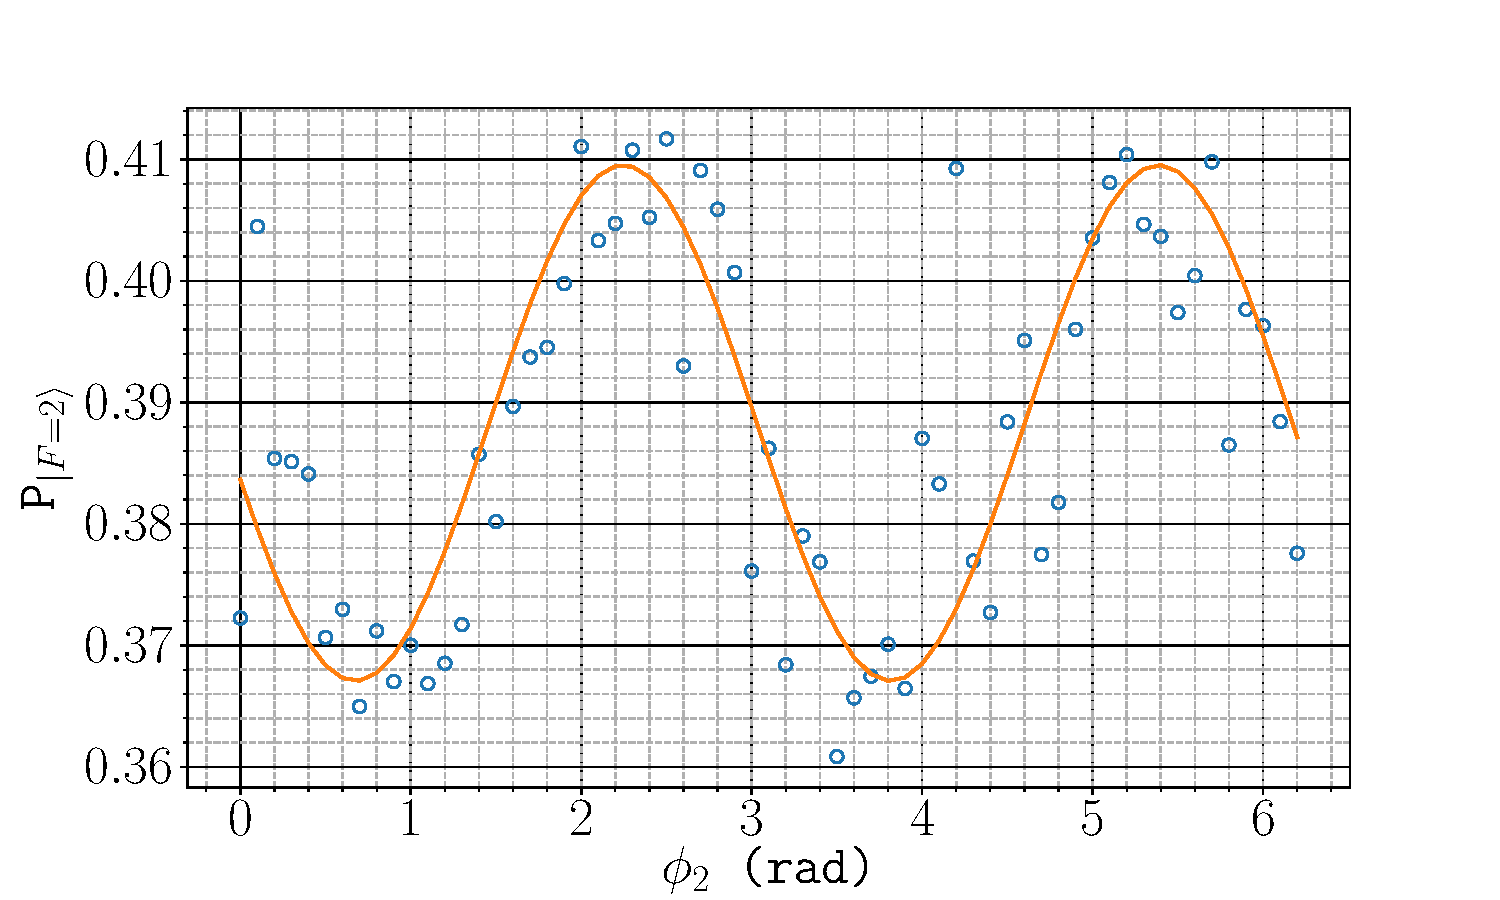
\includegraphics[width=0.6\textwidth]{fringe_examp}
  \caption[Interference fringe for \(T = \)\sivalue{25}{\ms}.]{Interference fringe obtained by varying the phase
    difference of the two Raman lasers during the middle \(\pi\) pulse
    for a pulse separation time of \(T = \)\sivalue{25}{\ms}. The orange
curve is a non-linear least squares fit to the data, giving a contrast
of \(C = 0.055\) and a mean value of \(\textnormal{P}_0 = 0.39\). The
shaded region indicates the 95\% confidence band. }
  \label{fig:fringe_examp}
\end{figure}

\subsection{Correcting for Vibration Noise}\label{sec:vibration_senstivity}
Vibrations of the retro-reflecting mirror are a significant source of
phase noise, which limits the sensitivity of the interferometer to
accelerations. This is particularly apparent when the vibration noise
induces a phase shift of greater than 2\(\pi\) radians. If the
interferometer signal spans multiple fringes, it is not possible to
accurately determine acceleration from the phase shift.
\par\noindent
One method to filter the effects of vibration noise, described in
~\cite{Merlet2009}, uses the MEMS accelerometer to measure the
vibration of the retro-reflecting mirror between the
first and last interferometer pulse. After this time, the phase shift
due to vibrations is given by the following convolution
\begin{equation}
  \phi_\textnormal{vib} = K \int_{-T}^{T} g_a (t) V(t) \mathrm{d}t = K
  \widetilde{V}_\textnormal{vib}
  \label{eq:phase_vib}
\end{equation}
where \(V(t)\) is the voltage measured across the output of the MEMS
accelerometer, \(K = \)\sivalue{0.793}{\m\s\tothe{2}\per\V} is the
scaling factor from voltage to acceleration and \(g_a(t)\) is the
acceleration sensitivity function, defined
in~\EquationRef{eq:acc_sens_approx}. The interferometer signal is then
fit to the function
\begin{equation}
  \text{P}_{\ket{F=2}} = \text{P}_0 + \frac{C}{2}\sin(\alpha
  \widetilde{V}_\textnormal{vib} + \phi_0)
  \label{eq:fringe_fit_vibration}
\end{equation}
\par\noindent
Common-mode suppression of the vibration phase noise is achieved by
estimating the interferometer phase from the residuals of the fit
to~\EquationRef{eq:fringe_fit_vibration}. If the interferometer phase
as estimated from~\EquationRef{eq:interferometer_phase} is denoted
\(\phi_\textnormal{int}\), then the fit residuals are
\(\phi_\textnormal{res} =  \phi_\textnormal{int} -
\phi_\textnormal{vib}\).
The correlation of the acceleration measured by the MEMS accelerometer
and the interferometer signal is shown
in~\FigureRef{fig:vib_comparison}. The Raman laser phase difference was
initially set so that the interferometer signal was at the mid-point
of the fringe \(\Delta \phi = \pi/2\) before continuously running the
experiment. The vibration noise was increased
by removing the pneumatic suspension of the optical table, which
helps to passively isolate the experiment from external vibrations
that are coupled through the table legs. Without this additional
suppression, the vibration noise is large enough to shift the
interferometer phase by more than \(2\pi\), as indicated
in~\FigureRef{fig:high_vib}. When the table is suspended, the
vibration noise is small enough that the interferometer signal remains
on one side of the fringe.
\begin{figure}[htpb!]
  \centering
  \subfloat[][]{\scalebox{0.5}{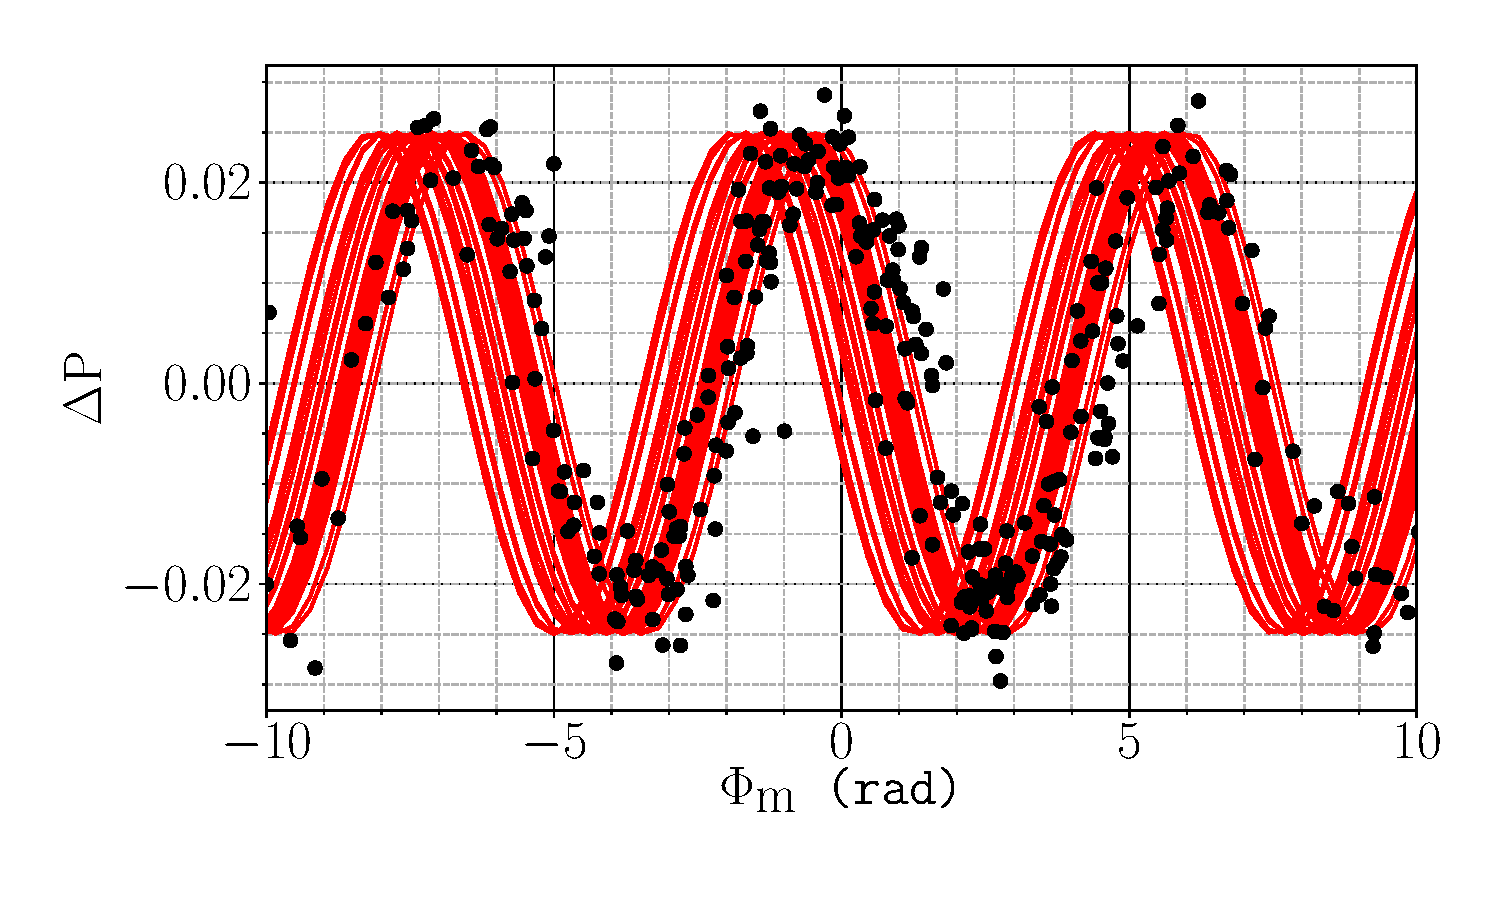
\includegraphics{high_vib}}\label{fig:high_vib}}
    \subfloat[][]{\scalebox{0.5}{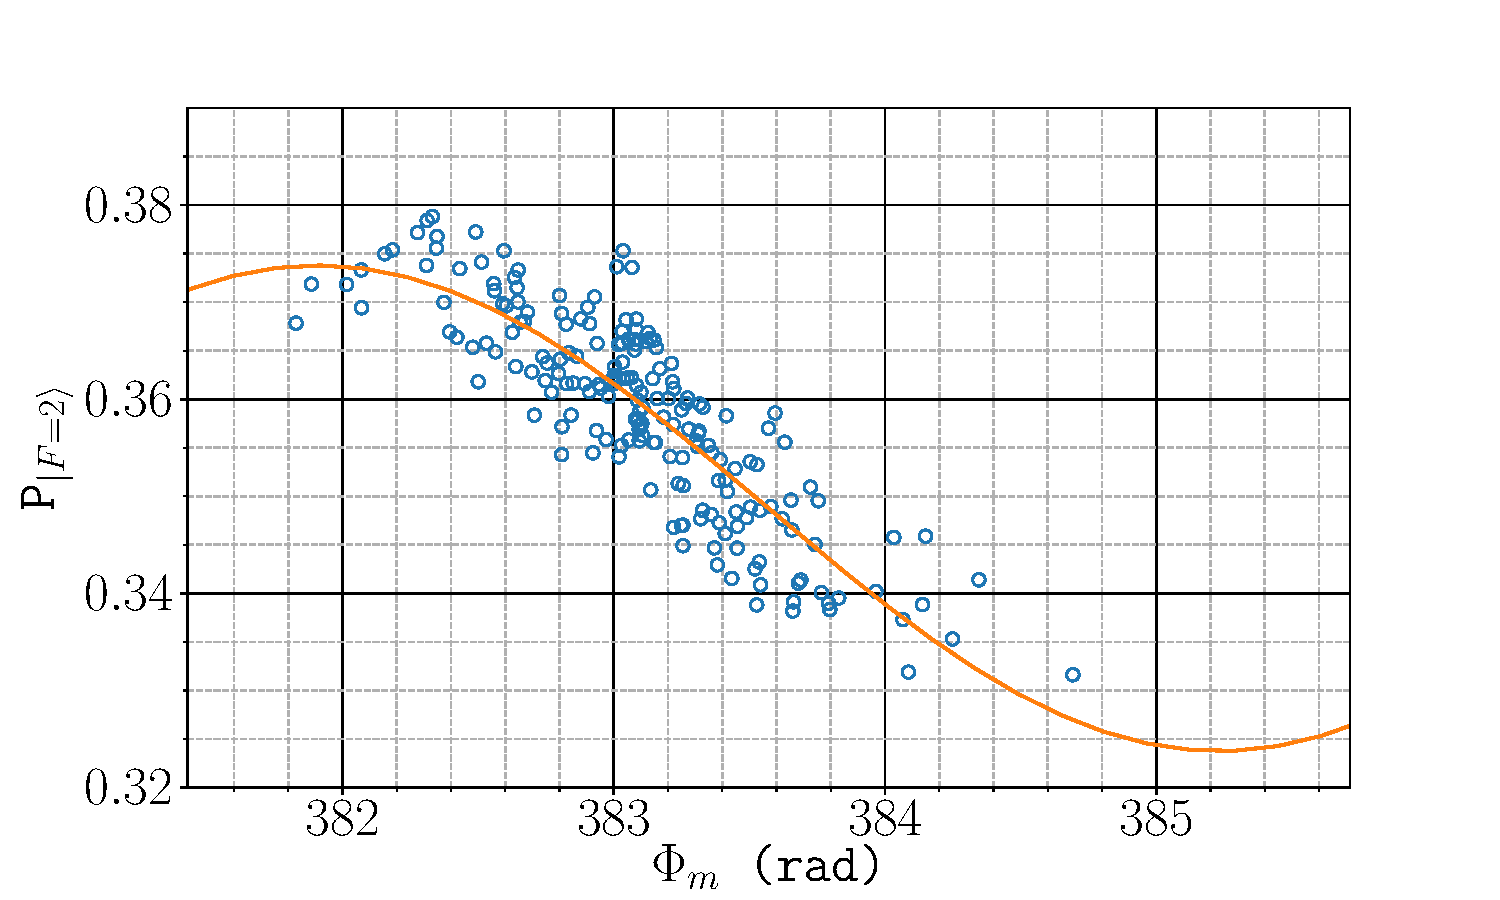
\includegraphics{low_vib}}\label{fig:low_vib}}
  \caption[Comparison of MEMS/Interferometer correlation in a high and
    low vibration
  environments.]{Correlation between acceleration measured by the MEMS
    accelerometer and the interferometer signal. \textbf{(a)} shows
    the correlation measured in high vibration environment, when the
    optical table was not pneumatically suspended. \textbf{(b)} shows
    the reduction in phase noise with this additional vibration
  isolation.}
  \label{fig:vib_comparison}
\end{figure}
\par\noindent
The suppression of the vibration noise can be seen in the distribution
of the estimated acceleration. For the data obtained when the
vibrations were more suppressed (\FigureRef{fig:low_vib}), histograms of the acceleration measured
by the MEMS accelerometer and the interferometer are shown
in~\FigureRef{fig:vibration_hists}.
\FigureRef{fig:low_vib_hist_mems_atom} compares the distribution of
the accelerations measured by the MEMS with that of the
interferometer. The  

\begin{figure}[htpb!]
  \centering
  \subfloat[][]{\scalebox{0.5}{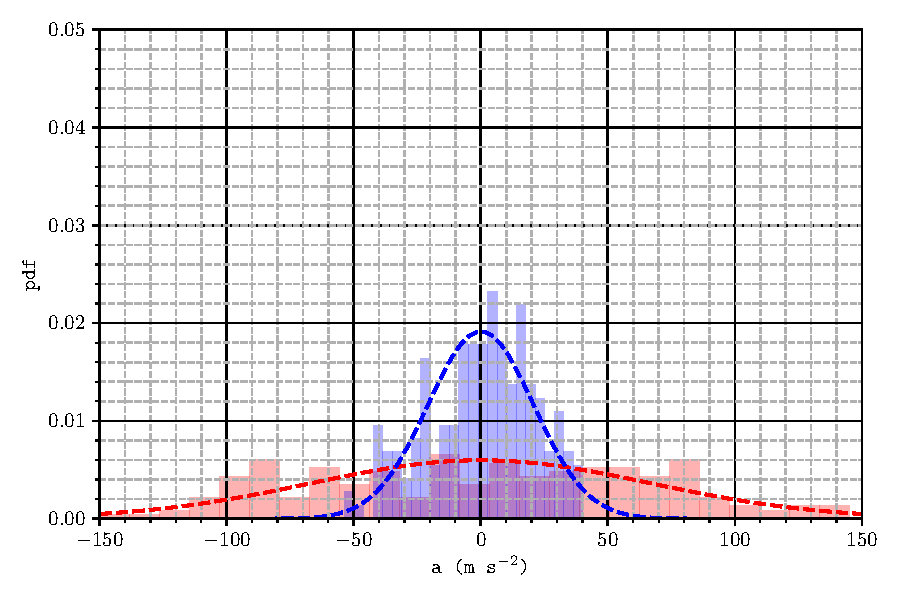
\includegraphics{low_vib_hist_mems_atom}}\label{fig:low_vib_hist_mems_atom}}
    \subfloat[][]{\scalebox{0.5}{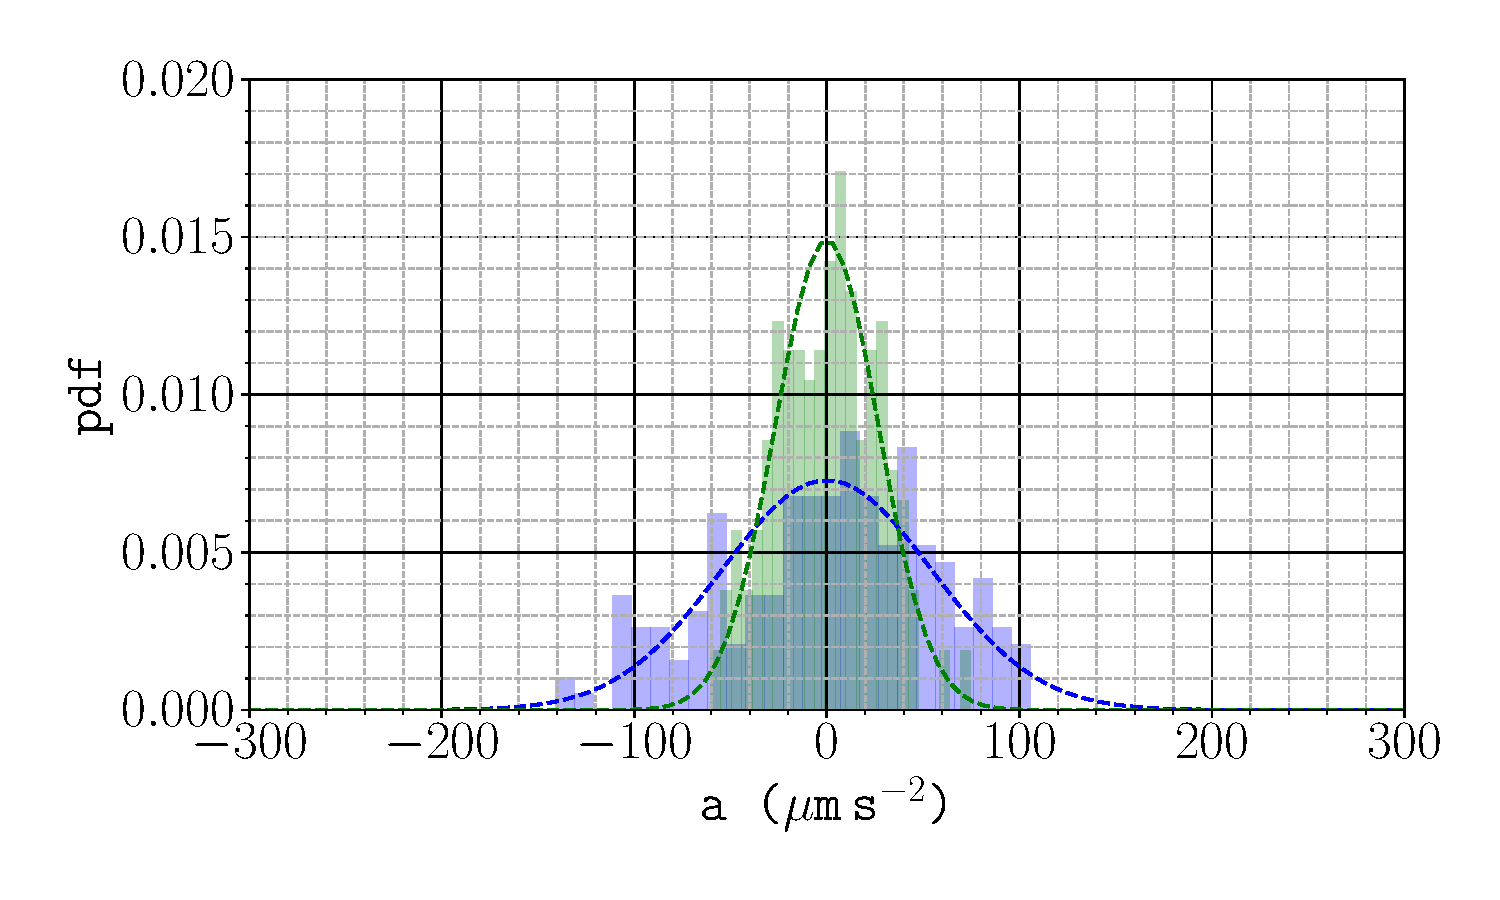
\includegraphics{low_vib_hist_atom_res}}\label{fig:low_vib_hist_atom_res}}
  \caption[Histogram of acceleration noise.]{Histograms of the
    acceleration noise about the mean value. \textbf{(a)} shows
    the distribution of the acceleration measured by the MEMS
    accelerometer (red) and the interferometer (blue). \textbf{(b)} shows
    the distribution after filtering the vibration noise from the
    interferometer signal (green). The dashed lines indicate the
  fitted normal distributions.}
  \label{fig:vibration_hists}
\end{figure}

\subsection{Signal Stability}\label{subsec:stability}	
The stability of the interferometer's sensitivity to accelerations can
be determined from the Allan deviation. A comparison of the
Allan deviation in the presence of high and low vibrations is shown
in~\FigureRef{fig:adev_comparison}. In both instances, the sensitivity
to accelerations is improved by correcting for the vibration-induced
phase. Under high vibration (\FigureRef{fig:high_vib_adev}), the Allan deviation has a minimum value
of around \sivalue{3e-6}{\m\s\tothe{-2}} after integrating for
\sivalue{35}{\s}. This is a bias instability, i.e. fluctuations in
the bias. This value is obtained by subtracting the vibration
phase, estimated from the MEMS accelerometer, from the interferometer
phase. It is possible that noise in the MEMS
accelerometer is contributing to a bias instability.
\par\noindent
When the vibration level is reduced, the signal
remains stable for a longer period of time. Here, the Allan deviation
is proportional to \(\tau^{-1/2}\), which is characteristic of
uncorrelated white phase noise. For longer integration times, the
small number of samples introduces a large uncertainty on the Allan
deviation in~\FigureRef{fig:low_vib_adev}. However, for integration
times up to \sivalue{100}{\s}, 
the sensitivity of the signal is not limited by the same bias
instability as in the presence of larger 
\begin{figure}[htpb!]
  \centering
  \subfloat[][]{\scalebox{0.5}{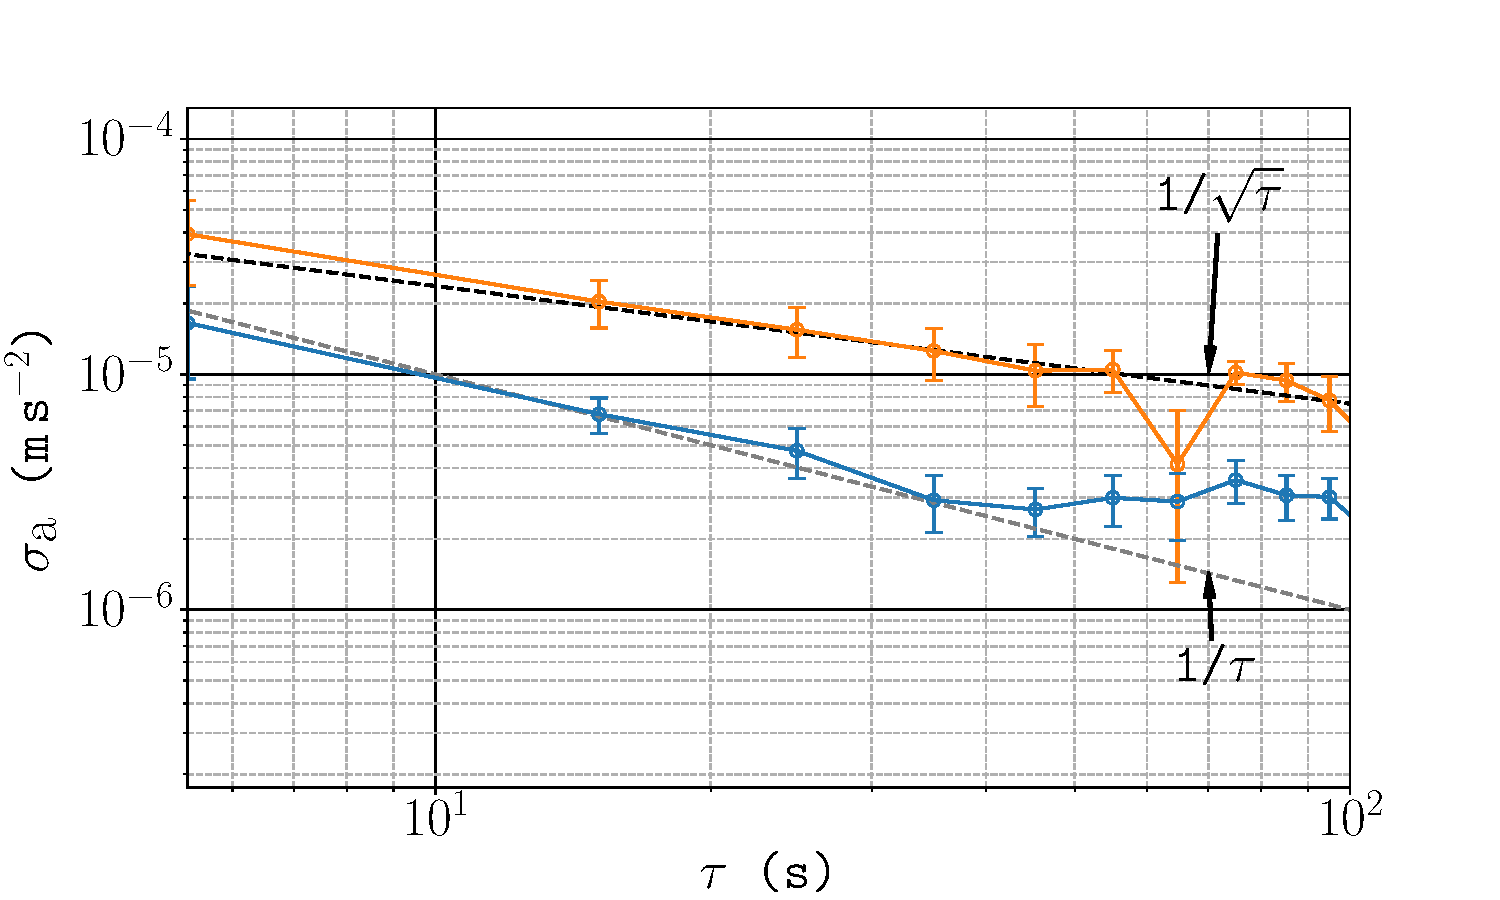
\includegraphics{high_vib_adev}}\label{fig:high_vib_adev}}
    \subfloat[][]{\scalebox{0.5}{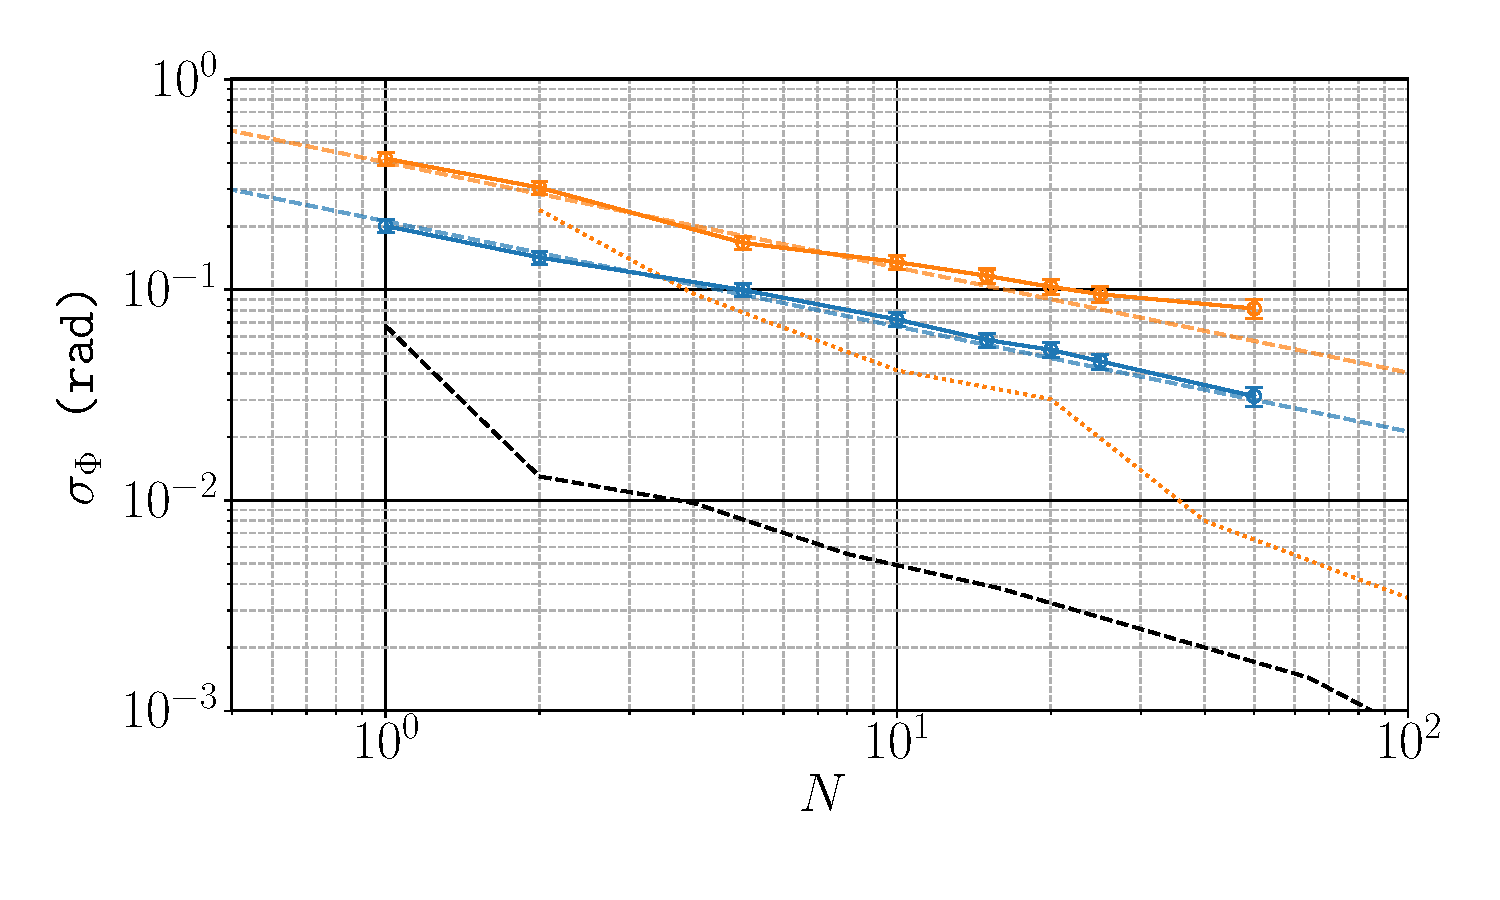
\includegraphics{low_vib_adev}}\label{fig:low_vib_adev}}
  \caption[Comparison of Allan deviation in a high and
    low vibration
  environment.]{Allan deviation of the estimated acceleration using
    the interferometer signal. In each plot the orange curve
    represents the sensitivity to accelerations without subtracting
    the vibration induced phase, and the blue curve shows the
    sensitivity after subtracting this. 
    As in~\FigureRef{fig:vib_comparison}, \textbf{(a)} shows
    the sensitivity in a high vibration environment, and
    \textbf{(b)} shows it after reducing the level of vibration.}
  \label{fig:adev_comparison}
\end{figure}
\section{Sensitivity}
This section presents a discussion of some of the major sources of
noise in the interferometer.
\subsection{The Allan Variance}
For the purposes of this experiment, the sensitivity of the
interferometer relates to the minimum value of uncertainty that can be
placed on a measurement of acceleration. As such, the limit to the
sensitivity is given by the measurement noise. One possible way to
characterise this is to use the variance. However with a finite sequence
of measurements, this depends on the number of samples and might not
converge as the number of samples increases. On the other hand, the
two-sample variance 
\begin{equation}
  \sigma_a^2(2,\tau) = \frac{1}{2}\left\langle
  (a_{n+1}-a_n)^2\right\rangle
  \label{eq:two_sample_var}
\end{equation}
does not depend on the number of samples. This can be generalized to
longer time separations \(t = N \tau\) by taking the mean of \(N\)
consecutive measurements
\begin{equation}
  \sigma_a^2(2,t) = \frac{1}{2}
  \left\langle
  \left(\frac{1}{N}\sum_{k=0}^{N-1}a_{n+1}-\frac{1}{N}\sum_{k=N}^{2N-1}a_n\right)^2\right\rangle
  \label{eq:allan_var_mean}
\end{equation}
which is referred to as the Allan variance~\cite{Allan1966}. If the noise in each measurement is uncorrelated, then this becomes
\begin{equation}
\sigma_a(2,t) = \frac{1}{\sqrt{N}}\sigma_a(2,\tau)
\label{eq:allan_var_simp}
\end{equation}
\par\noindent
The variance is also related to the signal-to-noise ratio of the
observed interferometer fringes. From the interferometer signal
defined in~\EquationRef{eq:interferometer_phase}, the variance at the
mid-point of the fringe \(\Delta \phi = \pi/2\) is given by
\begin{equation}
\sigma_P^2 = \sigma_{\text{P}_0}^2 +\frac{C^2}{4}
  \sigma_{\Delta \phi}^2
  \label{eq:var_expansion}
\end{equation}
The signal-to-noise ratio
\begin{equation}
  \left(\frac{S}{N}\right) = \frac{C}{2\sigma_P}
  \label{eq:snr}
\end{equation}
is the ratio of the fringe amplitude to the standard deviation of the
interferometer signal. Under the assumption that \(\text{P}_0\) and
\(C\) do not fluctuate, the signal-to-noise ratio is related to the
interferometer phase and acceleration uncertainties by
\begin{equation}
  \left(\frac{S}{N}\right)^{-1} = \sigma_{\Delta \phi} = \keff T^2 \sigma_a
  \label{eq:snr_acc}
\end{equation}

\subsection{Sources of Noise}
Some potential sources of noise have been investigated to determine
their magnitude. These are not a complete list of the effects which
reduce the sensitivity to accelerations, but are the most dominant. The
identified sources and their estimated effects on acceleration
measurements are shown in~\TableRef{tab:noise_sources}. The largest
contributor comes from vibrations of the retro-reflecting mirror.
Other noise sources, such as magnetic field gradients, laser intensity
noise and rotations have not yet been characterised.
\begin{table}[htpb!]
  \centering
  \begin{tabular}{c|c|c}
    \toprule
    Noise Source & Signal/Noise & \(\sigma_a\)
    (\sivalue{}{\micro\meter\per\s\squared}) \\
    \midrule
    Atom shot noise (\num{5e6} atoms) & 2200 & 0.07 \\
    Laser phase noise & 157 & 1 \\
    Detection noise & 15 & 10.5 \\
    Vibrations & 5.8 & 26\\
    \bottomrule
  \end{tabular}
  \caption{Comparison of known noise sources and their effects on
  acceleration measurements. These values are estimated assuming a
separation between pulses of \(T = \)\sivalue{25}{\ms} and a \(\pi/2\)
pulse time of \(\tau = \)\sivalue{20}{\micro\s}.}
  \label{tab:noise_sources}
\end{table}

%\subsection{Atom Shot Noise}

%subsection{Detection Noise}

\subsection{The Sensitivity Function}
The sources of noise presented thus far arise from statistical
uncertainties in measuring the number of atoms and are not present in
the ideal case of perfect interferometer contrast. However, there are
still other sources which introduce interferometer phase noise. Generally speaking, these add a random component to
the interferometer phase which is independent of the forces acting on
the atoms. Two dominant sources of phase noise are vibrations of the
retro-reflecting mirror and laser phase noise, i.e. fluctuations in
the relative phase between the two Raman light fields.
\par\noindent
The sensitivity function~\cite{Dick1987}
defines the instantaneous shift of the
interferometer phase \(\delta\Phi\) at a time \(t\) due to a phase
shift of the Raman laser phase \(\delta \phi\)
\begin{equation}
  g(t) = \lim_{\delta\phi \rightarrow 0} \frac{\delta\Phi(\delta \phi,
  t)}{\delta(\phi)}
  \label{eq:sensitivity_def}
\end{equation}
so the interferometer phase shift induced by fluctuations of
\(\phi\) is given by
\begin{align}
  \Phi &= \int_{-\infty}^\infty g(t)\delta \phi\;\mathrm{d}\phi(t)
  \nonumber\\
  &= \int_{-\infty}^\infty g(t)\;\frac{\mathrm{d}\phi}{\mathrm{d} t}\;
  \mathrm{d}t
  \label{eq:phase_contrib}
\end{align}
In the case of a \(\pi/2-\pi-\pi/2\) interferometer pulse sequence of
durations \(\tau_R-2 \tau_R - \tau_R\) and where \(t=0\) is defined at
the centre of the \(\pi\) pulse, the sensitivity function is 
\begin{equation}
    g(t) = 
    \begin{cases}
      \sin ( \Omega t) & 0<t<\tau_R  \\
      1 & \tau_R <t<\tau_R +T \\
      \sin (\Omega  (t-T)) & \tau_R +T<t<2 \tau_R +T
  \end{cases}
\label{eq:sensitivity_interferometer}
\end{equation}
for a pulse separation time \(T\). 
\subsection{Influence of Laser Phase Noise}
The response of the interferometer phase to laser phase noise is
best understood in the frequency domain. In particular, the inverse
of the interferometer pulse separation time 
The effects of \(\phi\) are best
thought of in terms of its Fourier components. Writing \(\phi(t) = A
\cos(\omega t + \psi)\), \EquationRef{eq:phase_contrib} becomes
\begin{equation}
  \Phi = - A \omega \cos(\psi) \int_{-\infty}^\infty g(t) \sin(\omega
  t) \mathrm{d} t
  \label{eq:phase_fourier}
\end{equation}
where the term proportional to \(\cos(\omega t)\) has been dropped,
since \(g(t)\) is an odd function. The integrand
in~\EquationRef{eq:phase_fourier} is proportional to the Fourier
transform of \(g(t)\)
\begin{equation}
  G(\omega) = -i \int_{-\infty}^{\infty} g(t) \sin(\omega t)
  \mathrm{d} t
  \label{eq:sensitvity_fourier}
\end{equation}
which using~\EquationRef{eq:sensitivity_interferometer}
becomes~\cite{Canuel2007}
\begin{equation}
  G(\omega) = \frac{4 i
  \Omega}{\omega^2-\Omega^2}\sin\left(\frac{\omega(T+2\tau)}{2}\right)\left(\cos\left(\frac{\omega(T+2\tau)}{2}\right)
  + \frac{\omega T}{2}\sin \left(\frac{\omega T}{2}\right)\right)
  \label{eq:sens_fourier_full}
\end{equation}
so~\EquationRef{eq:phase_contrib} becomes
\begin{align}
  \Phi &= -i A \cos(\psi) \;\omega G(\omega) \nonumber \\
  &= - A \cos(\psi) \lvert H(\omega)\rvert
  \label{eq:interfometer_fourier}
\end{align}
\par\noindent
A plot of the transfer function \(|H(\omega)|^2\) is presented
in~\FigureRef{fig:transfer_function} for
\(T= \)\sivalue{20}{\milli\second} and \(\tau
= \)\sivalue{20}{\micro\second}. The asymptotic properties of the
transfer function can be summarised as follows:
\begin{itemize}
  \item At low frequencies \(\omega \ll \Omega\), the transfer
    function is approximated by 
    \begin{equation}
      |H(\omega)|^2 \approx 16 \sin \left(\frac{\omega T}{2}\right)^4
    \end{equation}
    which is a periodic function that is zero at frequency multiples
    of \(1/\pi T\) \\
  \item At frequencies \(\omega \gg \Omega\), the transfer function is
    \begin{equation}
      |H(\omega)|^2 \approx 4 \frac{\Omega^2}{\omega^2}\sin
      \left(\omega T\right)^2
    \end{equation}
    which is zero at multiples of \(1/2\pi T\) and is a low-pass
    first-order filter.
\end{itemize}
\begin{figure}[htpb!]
  \centering
  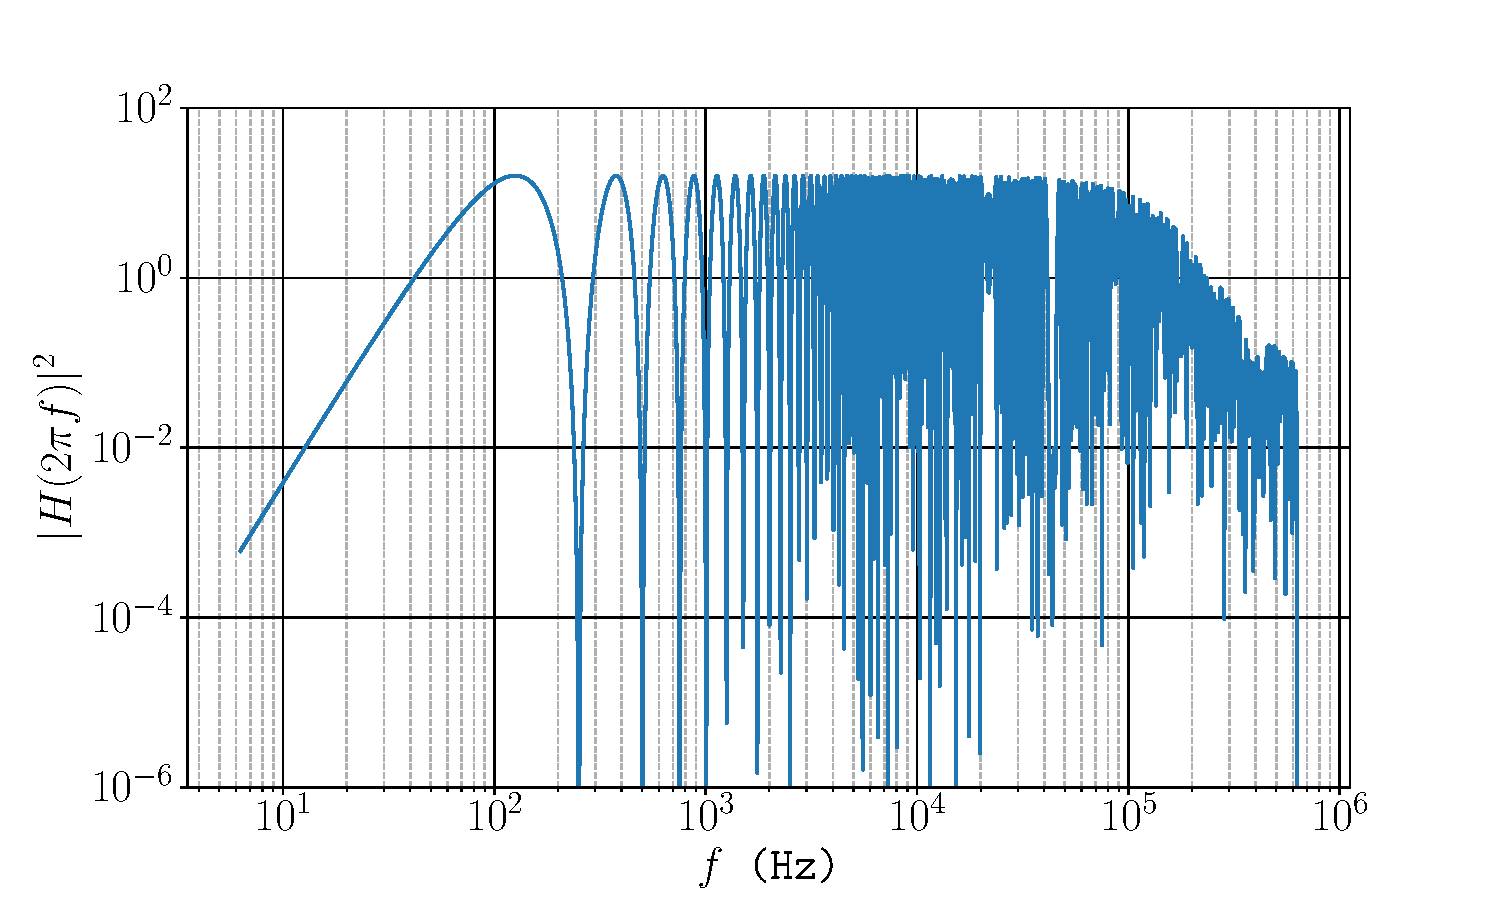
\includegraphics[width=0.6\textwidth]{transfer_func_laser.pdf}
  \caption[Transfer function for laser phase noise.]{Transfer function
  for laser phase noise. Here, the separation between pulses is \(T =
  \)\sivalue{20}{\milli\second} and the \(\pi/2\) pulse time is \(\tau
=\)\sivalue{20}{\micro\second}.}
  \label{fig:transfer_function}
\end{figure}
\par\noindent
The variance of \(\Phi\) is obtained by averaging over \(\psi\)
\begin{equation} 
  \sigma_\Phi^2 = \langle \Phi^2\rangle_\psi = \frac{1}{2} A^2
  |H(\omega)|^2
  \label{eq:var_phi_transfer}
\end{equation} which is related to the phase noise power spectral density
\(S_\phi(\omega)\) by
  \begin{equation}
    \sigma_\Phi^2 = \frac{1}{2}\int_{-\infty}^\infty
    S_\Phi(\omega)|H(\omega)|^2 \frac{\mathrm{d}\omega}{2\pi} =
      \int_0^\infty
    S_\Phi(\omega)|H(\omega)|^2 \frac{\mathrm{d}\omega}{2\pi} 
    \label{eq:phase_noise_psd}
  \end{equation}
Similarly, the Allan variance can be expressed using the transfer
function and the phase noise power spectral density~\cite{Gouet2008}.
The integration time \(\tau_\text{av} = m T_c\) is expressed in multiples
of the experiment cycling time \(T_c\). In the frequency domain, the phase
noise power spectral density is sampled at frequency multiples of
\(f_c = 1/T_c\), so the Allan variance becomes
\begin{equation}
  \sigma^2_\Phi(\tau_\text{av}) = \frac{1}{\tau_\text{av}}
    \sum_{k=1}^\infty |H(2\pi k f_c|)^2S_\phi(2\pi k f_c)
  \label{eq:avar_transfer}
\end{equation}
\par\noindent
The laser phase noise originates from the reference oscillator used in
the phase-locked loop for the M-Squared laser. The phase noise
spectral density and corresponding Allan deviation for increasing
integration time was measured by M-Squared during installation of the
laser system. A plot of the Allan deviation is shown
in~\FigureRef{fig:allan_dev_m_squared}. At an interferometer pulse
separation of
\(T = \)\sivalue{25}{\milli\second}, the phase noise in the Raman
laser results in an uncertainty in the interferometer phase of
\sivalue{10}{\milli\radian}. 
\begin{figure}[htpb!]
  \centering
  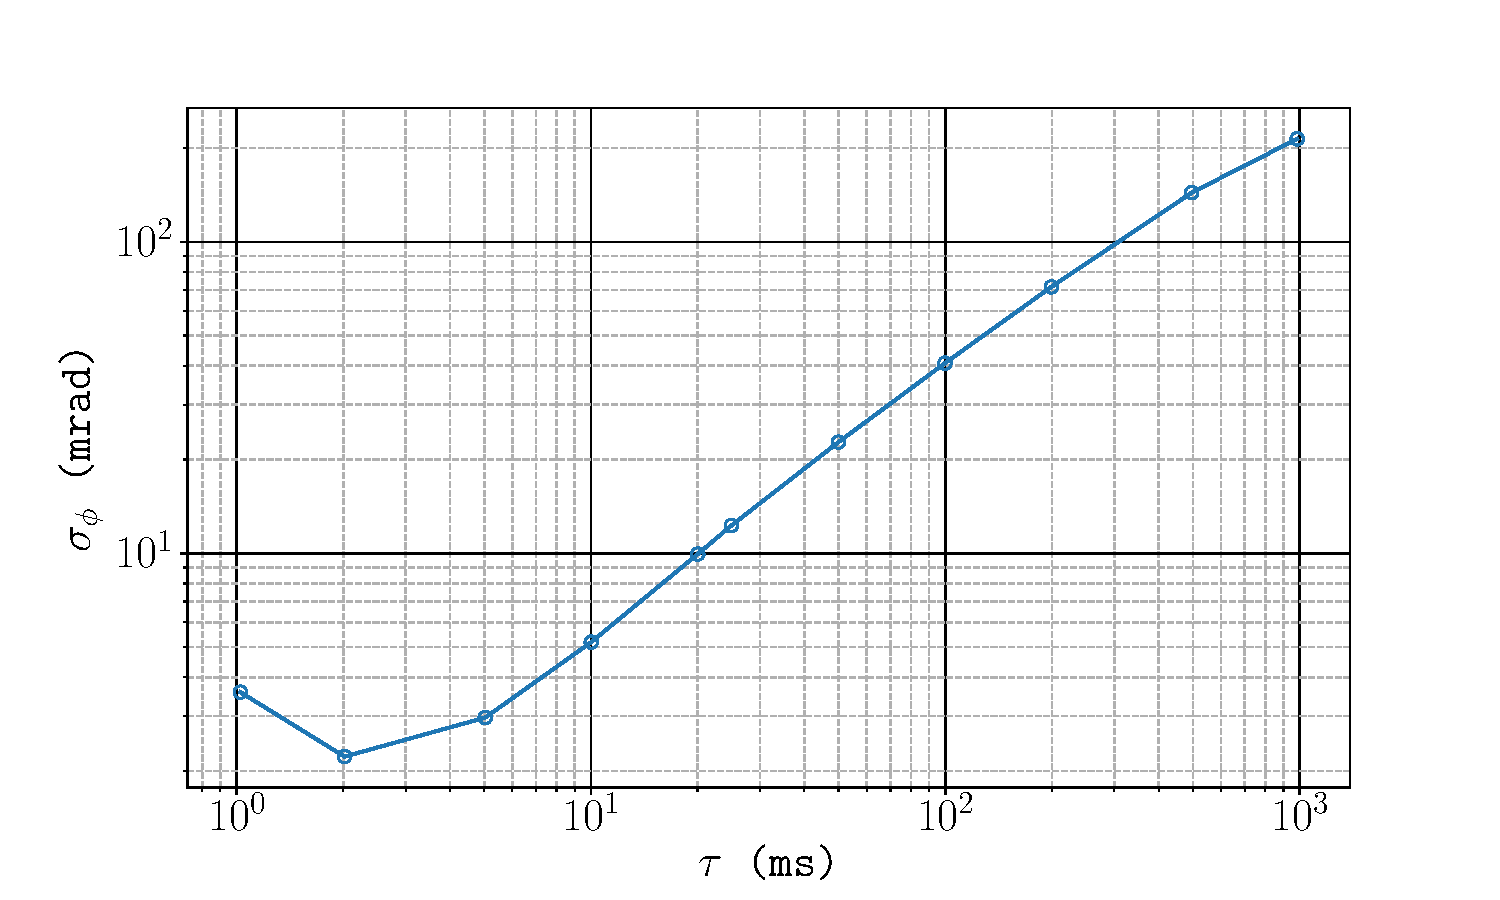
\includegraphics[width=0.6\textwidth]{allan_dev_m2.pdf}
  \caption[Allan deviation of the Raman laser phase difference.]{Allan deviation of the Raman laser phase difference for increasing integration time. Data reproduced from~\cite{M2_manual}.}
  \label{fig:allan_dev_m2}
\end{figure}


\subsection{Vibrations}
The phase difference between the two Raman beams depends on the
position of the retro-reflecting mirror. Consequently, this defines a frame of
reference for the position of the atoms during the interferometer. Any
random motion of the mirror, for instance from mechanical vibrations,
introduces a random component to the laser phase. An acceleration of
the mirror modifies the laser phase as follows
\begin{equation}
  \frac{\mathrm{d}^2 \Phi(t)}{\mathrm{d} t^2} = \keff.\textbf{a}(t)
  \label{eq:phase_acc}
\end{equation}
and the sensitivity to accelerations \(g_a\) is given by
\begin{equation}
  \frac{1}{k_\text{eff}} \frac{\mathrm{d}^2 g_a(t)}{\mathrm{d} t^2} =
  g(t) \\
  \label{eq:acc_sens}
\end{equation}
Assuming that the pulse time \(\tau\) is much shorter than the
interferometer pulse separation, \(T\), the acceleration sensitivity
function is approximated by
\begin{equation}
  g_a(t) = \begin{cases}
 -1 && - T < t < 0\\
 1 && 0 < t < T
  \end{cases}
  \label{eq:acc_sens_approx}
\end{equation}
From this, the acceleration transfer function is
\begin{equation}
  |H_a(\omega)|^2 = \frac{k_\text{eff}^2}{\omega^2}|H(\omega)|^2 
  \label{eq:acc_transfer}
\end{equation}
which in the low frequency limit \(\omega \ll \Omega\) is
\begin{equation}
  |H_a(\omega)|^2 = \frac{16 k_\text{eff}^2}{\omega^4}
  \sin\left(\frac{\omega T}{2}\right)^4
  \label{eq:acc_tf_low}
\end{equation}
Equivalent definitions for the variance and Allan variance are
obtained using this and the acceleration noise spectral density
\(S_a(2\pi f)\) as the respective definitions
in~\EquationRef{eq:phase_noise_psd}
and~\EquationRef{eq:avar_transfer}. The transfer function for
acceleration noise is shown in~\FigureRef{fig:transfer_func_acc}. The
gain is largest at low frequencies and approximates a second-order
filter at higher frequencies.
\begin{figure}[htpb]
  \centering
  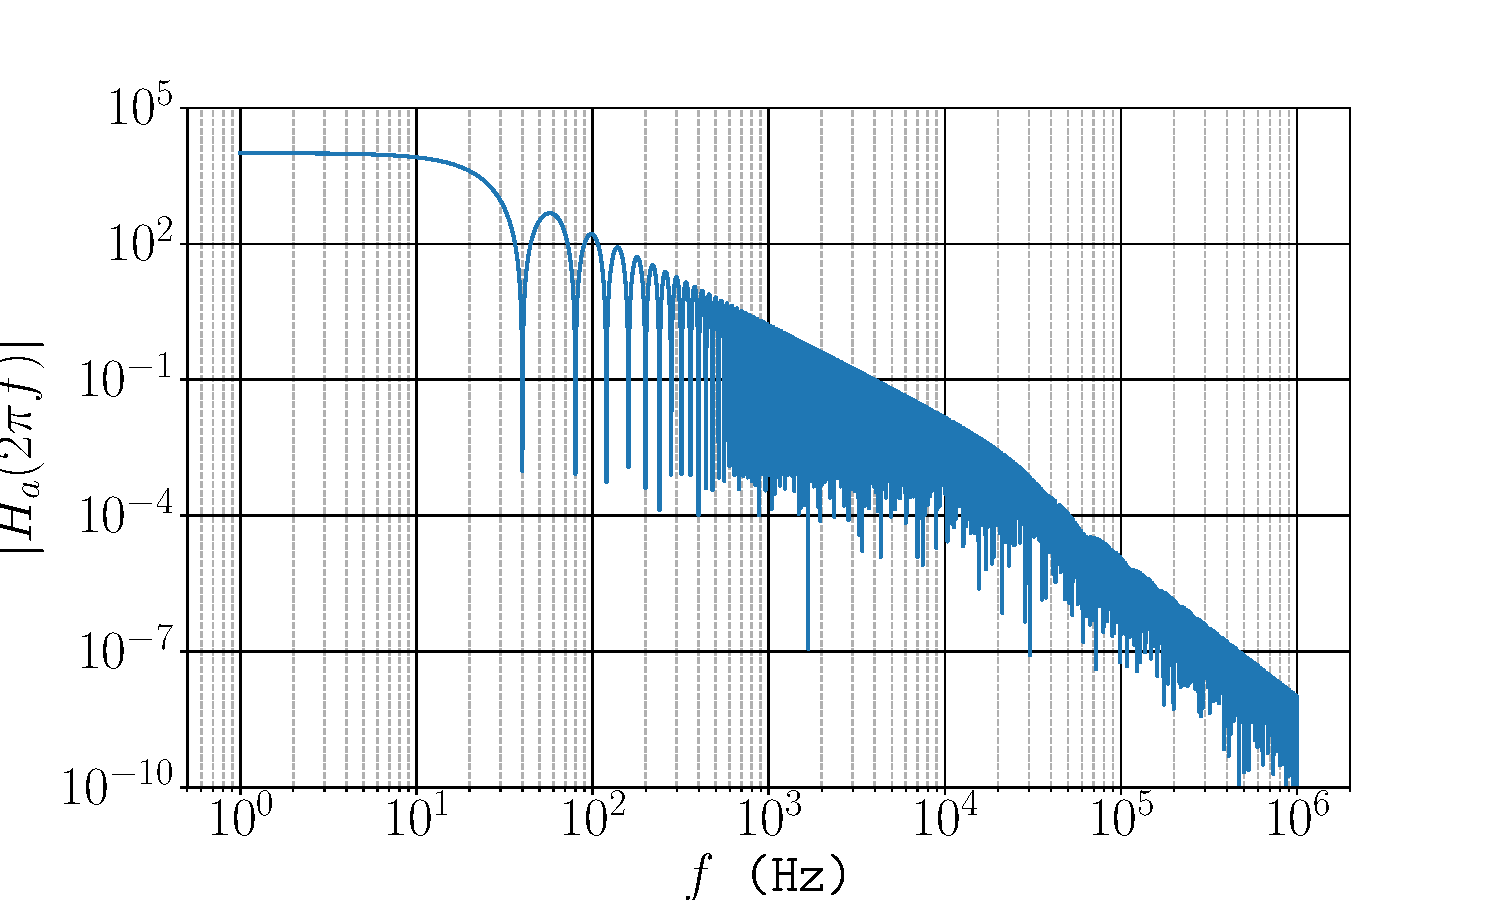
\includegraphics[width=0.6\textwidth]{transfer_func_acc}
  \caption[Acceleration noise transfer function.]{Acceleration noise
  transfer function. The parameters used here are the same as those
previously defined for~\FigureRef{fig:transfer_function}.}
  \label{fig:transfer_func_acc}
\end{figure}
\subsubsection{Measuring the Acceleration Noise Power Spectral Density}
The interferometer phase is most sensitive to low-frequency
vibrations. Acceleration noise at frequencies greater than \(1/2T\)
will mostly average out, contributing little to an overall phase.
Precise measurements of the interferometer phase rely on reducing the
low frequency noise. The vibration of the retro-reflecting mirror is
reduced by passively isolated it from its environment. The
chamber is mounted on a layer of Sorbothane to dissipate the
vibrations from the ground. This isolation is enhanced by a
pneumatic suspension system between the optical table and its
supporting legs. 
\par\noindent
A comparison of the acceleration noise spectral density with and
without the pneumatic suspension, measured using
the accelerometer mounted behind the retro-reflecting mirror, is shown
in~\FigureRef{fig:vibration_spectrum}. The suspension acts as a
low-pass filter and reduces the power within the
10-\sivalue{200}{\hertz} bandwidth, which is aliased into the lower
frequency band. For an interferometer pulse separation of \(T =
\)\sivalue{25}{\ms}, the
vibration phase noise using~\EquationRef{eq:avar_transfer} is \(\sigma_\Phi = \)\sivalue{270}{\milli\radian}. Without
floating the table, this becomes \sivalue{7}{\radian}. With the
vibration isolation systems currently used, this remains the dominant
source of phase noise. More sophisticated methods of damping
low-frequency vibrations are required to improve the interferometer's
acceleration sensitivity. 
\begin{figure}[htpb!]
  \centering
  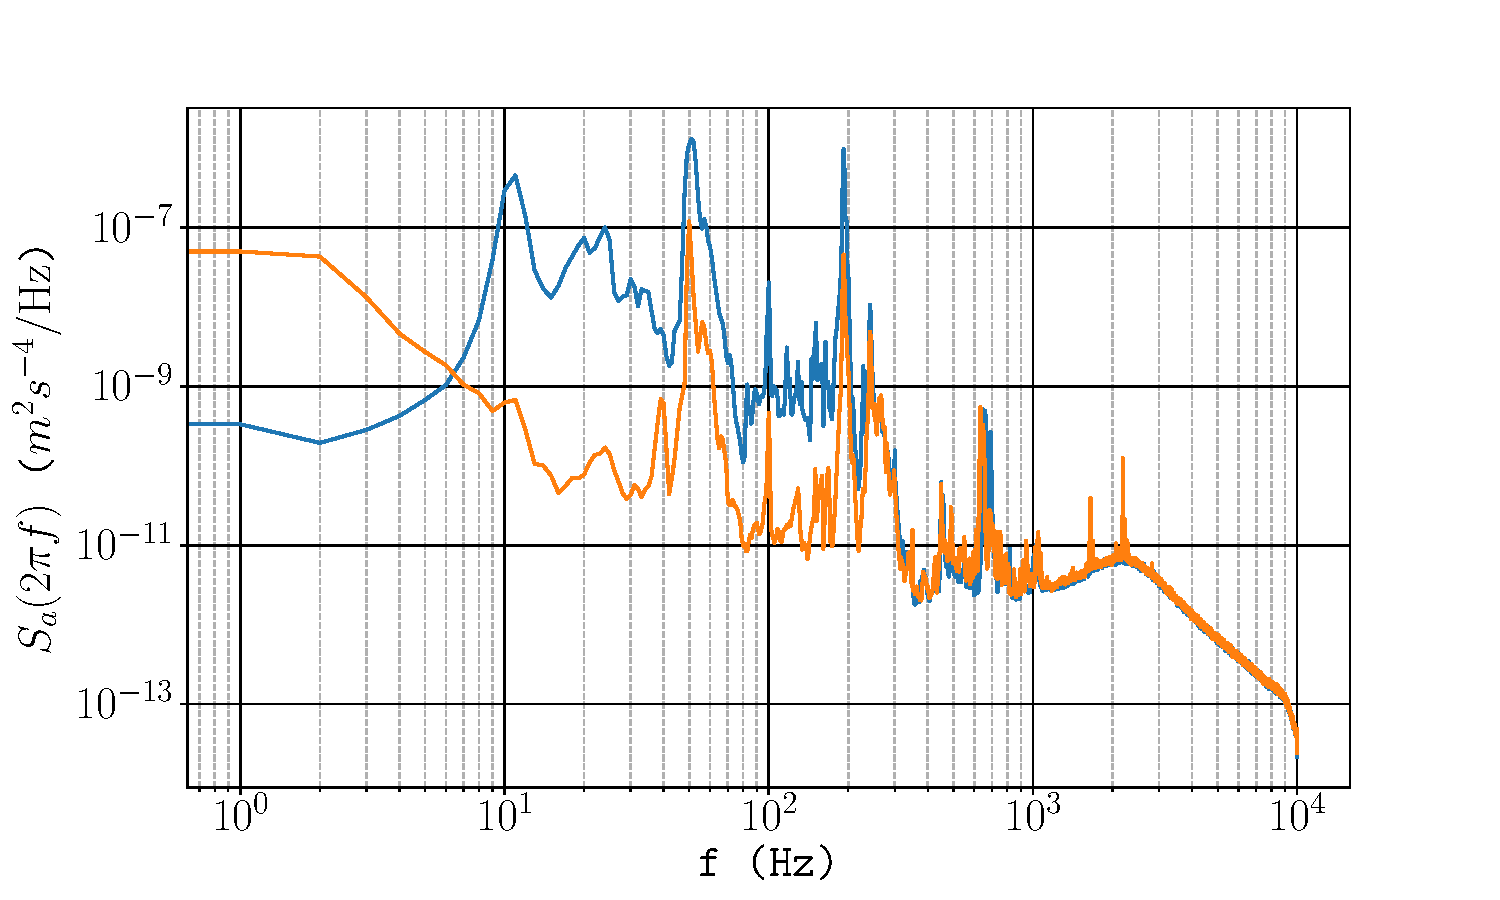
\includegraphics[width=0.6\textwidth]{vibration_spectrum.pdf}
  \caption[Acceleration noise power spectral density.]{Acceleration
  noise power spectral density sampled at a rate of
\sivalue{20}{\kilo\hertz}. The orange curve shows the acceleration
power spectral density using pneumatic suspension to decrease the
coupling of vibrations from the ground to the experiment. For
comparison, the blue curve shows the power spectral density without
this isolation.}
  \label{fig:vibration_spectrum}
\end{figure}

%\subsection{Other Sources of Phase Noise}
%Aside from laser phase noise and vibrations, there are additional effects
%which result in interferometer phase noise. These have not been
%characterised in this experiment as their magnitude is typically much
%smaller than the present vibration phase noise. 
%\begin{itemize}
%  \item \underline{Magnetic field gradients}. The \(\Delta_m = 0\)
%    clock transition has a second-order Zeeman shift of
%    \sivalue{575}{\Hz\gauss\tothe{-2}}. A gradient of magnetic field
%    across the area traversed by the atoms introduces a propagation
%    phase which does not cancel. 
%  \item \underline{Laser intensity noise}.
%\end{itemize}
